\documentclass{report}

\usepackage{amsmath, amsthm, amssymb, amsfonts}
\usepackage{thmtools}
\usepackage{graphicx}
\usepackage{setspace}
\usepackage{geometry}
\usepackage{float}
\usepackage{hyperref}
\usepackage[utf8]{inputenc}
\usepackage[english]{babel}
\usepackage{framed}
\usepackage[dvipsnames]{xcolor}
\usepackage{tcolorbox}
\usepackage{multicol}
\usepackage{subfig}
\usepackage{wrapfig}

\colorlet{LightGray}{White!90!Periwinkle}
\colorlet{LightOrange}{Orange!15}
\colorlet{LightGreen}{Green!15}

\newcommand{\HRule}[1]{\rule{\linewidth}{#1}}

\declaretheoremstyle[name=Theorem,]{thmsty}
\declaretheorem[style=thmsty,numberwithin=section]{theorem}
\tcolorboxenvironment{theorem}{colback=LightGray}

\declaretheoremstyle[name=Proposition,]{prosty}
\declaretheorem[style=prosty,numberlike=theorem]{proposition}
\tcolorboxenvironment{proposition}{colback=LightOrange}

\declaretheoremstyle[name=Principle,]{prcpsty}
\declaretheorem[style=prcpsty,numberlike=theorem]{principle}
\tcolorboxenvironment{principle}{colback=LightGreen}

\setstretch{1.2}
\geometry{
    textheight=9in,
    textwidth=5.5in,
    top=1in,
    headheight=12pt,
    headsep=25pt,
    footskip=30pt
}

% ------------------------------------------------------------------------------
\tcbset{
    sharp corners,
    colback = white,
    before skip = 0.2cm,    % add extra space before the box
    after skip = 0.5cm      % add extra space after the box
}                           % setting global options for tcolorbox

\definecolor{main}{HTML}{5989cf}    % setting main color to be used
\definecolor{sub}{HTML}{cde4ff}     % setting sub color to be used

\newtcolorbox{boxH}{
    colback = sub, 
    colframe = main, 
    boxrule = 0pt, 
    leftrule = 6pt % left rule weight
}

\newcommand{\SubItem}[1]{
    {\setlength\itemindent{15pt} \item[-] #1}
}

% ------------------------------------------------------------------------------

\begin{document}

% ------------------------------------------------------------------------------
% Cover Page and ToC
% ------------------------------------------------------------------------------

\title{ \normalsize \textsc{}
		\\ [2.0cm]
		\HRule{1.5pt} \\
		\LARGE \textbf{\uppercase{Hardware and Device-to-Device Communication Security}}
		\HRule{2.0pt} \\ [0.6cm] \LARGE{Notes about that} \vspace*{10\baselineskip}}
\date{}
\author{\textbf{Fabio Lorenzato}} 
		

\maketitle
\newpage

\tableofcontents
\newpage

% ------------------------------------------------------------------------------

% \section{Examples}

% \begin{theorem}
%     This is a theorem.
% \end{theorem}

% \begin{proposition}
%     This is a proposition.
% \end{proposition}

% \begin{principle}
%     This is a principle.
% \end{principle}

% Maybe I need to add one more part: Examples.
% Set style and colour later.

% \newpage
\part{Wireless}
\chapter{Digital Communication}
This first section is all about how to convert and transmit some signal.
\begin{section}{Introduction}
\label{sec:intro}
The goal of communication is to transmit some kind of data form a sender to a receiver. In order 
to do so, the physical layer defines the means of transmitting a stream of \textbf{raw bits} over a
physical data link, which connects those two nodes.\\
Data is transmitted in the form of \textbf{signals}, which are a physical representation of the data.
The signal is transmitted over a \textbf{channel}, which is the transmission medium that connects 
the sender and receiver. This can be both wired or wireless.\\
% Whereas with wired channels, checking the device connected to the channel is easier to implement, 
% with wireless ones security is a major when travelling in the channel. This is for may reasons:
In wired channels, it is really easy to check which devices are connected to the channel, on the
other hand, in wireless channels the communication is broadcast, and security becomes a major
concern. This is for many reasons:
\begin{itemize}
  \item No inherent protection is applied to the channel( it is replaced by a logical association)
     \subitem sending and receiving messages do not need physical access to the network 
     infrastructure
  \item the communication is in broadcast, which is intrinsic of radio nature.
    \subitem Transmission can be overheard by anyone in range( which can be quite big, depending 
    on the situation), and anyone can generate a transmission, for example by jamming nearby 
    transmissions.
\end{itemize}
As a result:
\begin{itemize}
  \item Eavesdropping is easy
  \item Injecting fake messages into the communication in easy
  \item replaying previously recorded messages is easy(\textit{meaconing}). This is actually very 
    dangerous for gps positioning, so it is also a security concern.
  \item illegitimate access to the network and its services is easy
  \item Denial of service attacks are easy, achieved by jamming the channel.
\end{itemize}
% 9/43
\end{section}
\begin{section}{Digital Communication System}
The digital communication system in characterized by three sections: 

\begin{itemize}
  \item the \textbf{user section}, which consist in the transmitter and the receiver, that want to 
    communicate. 
  \item the \textbf{interface section}, which is the interface to conveying the signal from the 
    user to the analog channel. It also transforms bits to analog signal, compressing and encoding 
    them, also associating bits to signal waveforms, to transform bits to analog signal.
  \item the \textbf{channel section}, which is the physical medium, that can only propagate analog 
    waveforms. In the end, we want to transmit digital signal but we are forced to use analog ones.
\end{itemize}

\begin{figure}[h]
  \centering
  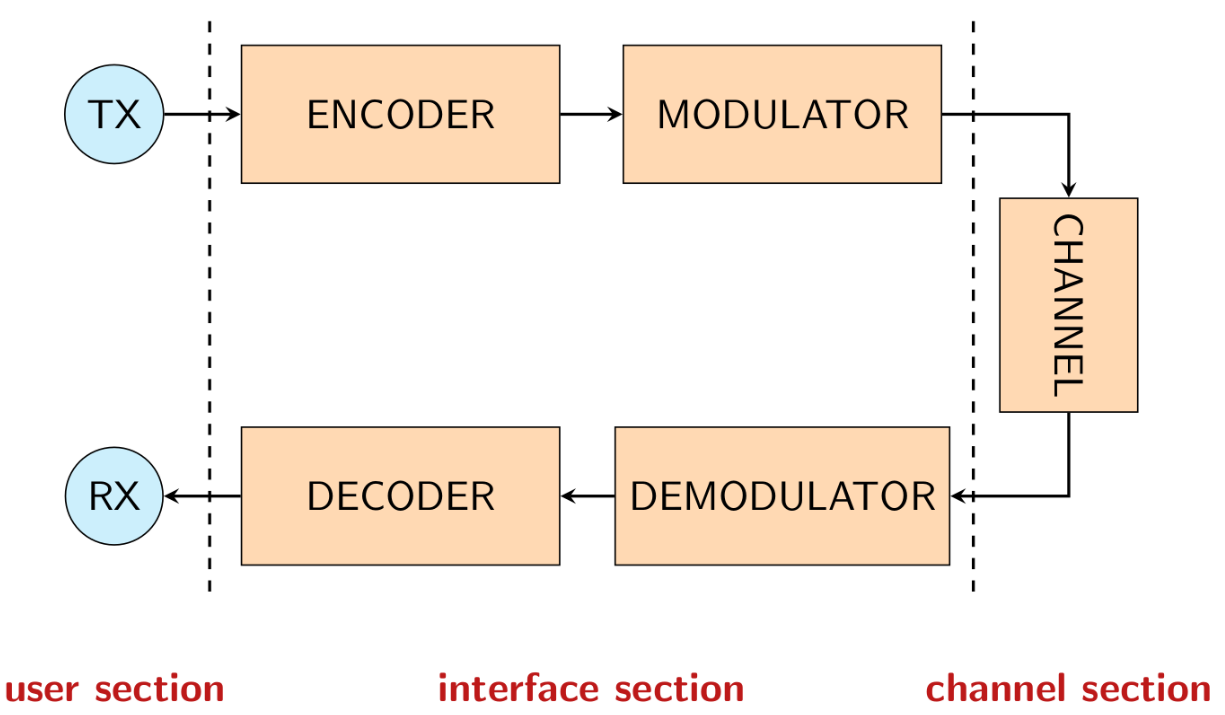
\includegraphics[width=0.7\textwidth]{img/wireless/digital communication schema.png}
  \caption{Digital Communication System}
  \label{fig:Digital Communication System}
\end{figure}
\begin{subsection}{The transmitter chain}
The transmitter chain is the part of the system that takes the digital signal, or an analog one 
converted to digital, and converts it to an analog signal, that can be transmitted over the
channel.\\
It is basically composed by two parts. The first one being an \textbf{encoder}, which can limit the amount 
of bits transmitted(\textit{source encoding}), and/or make the transmitted sequence more robust to
errors(\textit{channel encoding}).\\
The second one is the \textbf{modulator}, which is the part of the system that takes the digital
signal and converts it to an analog one to transmit it over the channel.
\end{subsection}

\begin{subsection}{The channel}
  \label{subsec:channel}
The channel is the physical medium that transfers bits from interface to interface, from the sender
to the receiver.
Its operation is affected by different types of disturbances such as:
\begin{itemize}
	\item frequency-domain distortion
	\item wireless fading
	\item additive noise
	\item impulsive noise
	\item interference from other frequency channels (interchannel interference)
	\item interference from the same frequency channel (cochannel interference)
	\item Intentional interference
\end {itemize}
\end{subsection}
\begin{subsection}{The receiver chain}
The receiver chain is the part of the system that takes the analog signal from the channel and
converts it to a digital signal, that can be processed by the user.\\
It is composed by the dual counterpart of the transmitter chain, the \textbf{demodulator} and the
\textbf{decoder}. \\
The demodulator takes the analog signal and converts it to a sequence of samples that can be
processed by the decoder.\\
The decoder takes the sequence of samples and converts it to a digital signal. It implements
\textit{channel decoding}, to correct errors, and \textit{source decoding}, to recover the original
message.
\end{subsection}
\end{section}

\begin{section}{Signal representation and Processing}
  \begin{boxH}
    A \textbf{signal} is a (mathematical) function that conveys information about a phenomenon.
  \end{boxH}
  Basically, any quantity that varies over space or time can be used to represent a informations,
  allowing to describe the evolution of physical quantities over time(voltages, currents, \dots).\\
  Its mathematical representation is therefore a function of real variable (time) taking real or 
  complex(more than one) values.\\
  We will be mostly focused on Electromagnetic Signals (e.g. voltage), but the general concepts 
  can be applied to any kind of signal
  \begin{subsection}{Energy of a signal}
    The energy of a signal is the integral of the squared modulus of the signal itself.
    \begin{equation}
      E(x) = \int_{-\infty}^{\infty} |x(t)|^2 dt
    \end{equation}
    As we can see , the energy is a scalar value, and the whole function is made positive by the
    squared modulus.\\
    \begin{figure}[h]
      \centering
      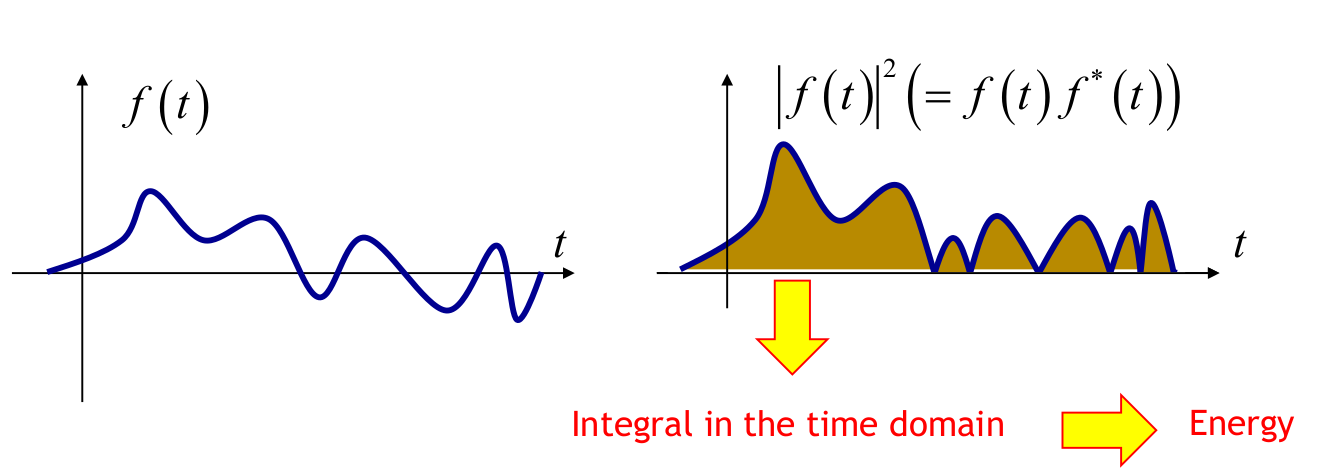
\includegraphics[width=0.7\textwidth]{img/wireless/energy signal.png}
      \caption{Energy of a signal}
      \label{fig:Energy of a signal}
    \end{figure}
    A signal with a very large amplitude, over time, will have a very high energy, while a signal
    which assumes values close to zero will have a very low energy, being a very weak signal.\\
    Furthermore, we can notice that the higher the distance of the signal from the origin, the
    larger the energy.
  \end{subsection}
  \begin{subsection}{Power of a signal}
    When we refer to power we can refer to the \textbf{instantaneous power} of a signal, which is just the 
    square module of a signal
    \begin{equation}
      P(x) = |x(t)|^2
    \end{equation}
    but much more commonly we refer to the average power of a signal, which is the time average of
    the instantaneous power of the whole signal.
    \begin{equation}
      P(x) = \lim_{a \to \infty} \frac{1}{2a} \int_{-a}^{a} |x(t)|^2 dt
    \end{equation}
    This a again a scalar value.
  \end{subsection}
  \begin{subsection}{Signal Representation}
    To analyze and process the signals, it is necessary to adequately represent them, and the
    definition of signals as "time functions" is NOT effective for many applications, for many 
    reasons.\\
    Generally, signals can become very complicated depending on our communication system, and
    we want different ways of representing them, to make them easier to process.\\
    For instance, we can represent a signal as a sum of elementary signals, thanks to the scalar
    product of the signal with a basis of the space of signals.\\

    The scalar product between signals is a scalar value, which is a measure of the similarity 
    among signals.\\
    If two function are quite similar we will get a large number.
    It it is zero, they are said to be orthogonal.
    \begin{equation}
      \langle x,y \rangle = \langle x(t),y(t) \rangle = \int_{-\infty}^{\infty} x(t)y^*(t) dt
    \end{equation}

    So, if we have a set of elementary signals $w_1(t), w_2(t), \dots, w_m(t)$, we write the signal
    $x(t)$ as a linear combination of the elementary signals:
    \begin{equation}
      x(t) = \sum_{i=1}^{m} \alpha_i w_i(t)
    \end{equation}
    where $\alpha_i$ are the coefficients of the linear combination $\alpha_i = \langle x(t), 
    w_i(t) \rangle$.\\
    In a more down to hearth way, the coefficient $\alpha_i$ allows us to understand how much each
    individual signal is similar to any other elementary signal we are considering, and because the 
    scalar product is higher for similar signals, we can understand how much each elementary signal
    is contributing to the whole signal.\\

    Furthermore, by adjusting the coefficient, we are able to create a whole different signal using
    the same elementary signals.
    \begin{subsubsection}{A common example: In Phase and Quadrature components representation}
      \label{sub:IQ representation}
      Lets consider a very simple basis, or a set of elementary signals, which is actually more 
      important that many other ones:
      \begin{itemize}
        \item the \textbf{in-phase} signal, which, in this case, is a cosine function $w_1(t) = cos(2\pi f_o t)$
        \item the \textbf{quadrature} signal, which, in this case, is a sine function $w_2(t) = sin(2\pi f_o t)$
      \end{itemize}
      where $f_o$ is the frequency, in Hz, of the signal.\\
      We can write any signal as a linear combination of these two signals, just by adjusting the
      coefficients:
      \begin{equation}
        x(t) = x_1 cos(2\pi f_o t) + x_2 sin(2\pi f_o t)
      \end{equation}
      where x(t) is the signal we want to represent, and $x_1$ and $x_2$ are the coefficients of the
      linear combination.\\

      A very simple representation of this complex signal is obtainable by representing each signal 
      as an axes in a complex plane, for example in figure \ref{fig:Complex Plane} the x-axis 
      is the in-phase signal, and the y-axis is the quadrature signal.\\
      Each signal can be represented as a point in the complex plane, because the distance from the
      origin signal(\textit{axis}) is the amplitude of the signal.\\
      This kind of representation is called the \textbf{In-phase and Quadrature} representation, or
      \textbf{I/Q} representation.\\
      For example, choosing a point close to the x-axis, we are choosing a signal with a very low
      quadrature component, and a very high in-phase component.Furthermore, a set of those 
      different points is called a \textit{constellation}\\
      \begin{figure}[h]
        \centering
        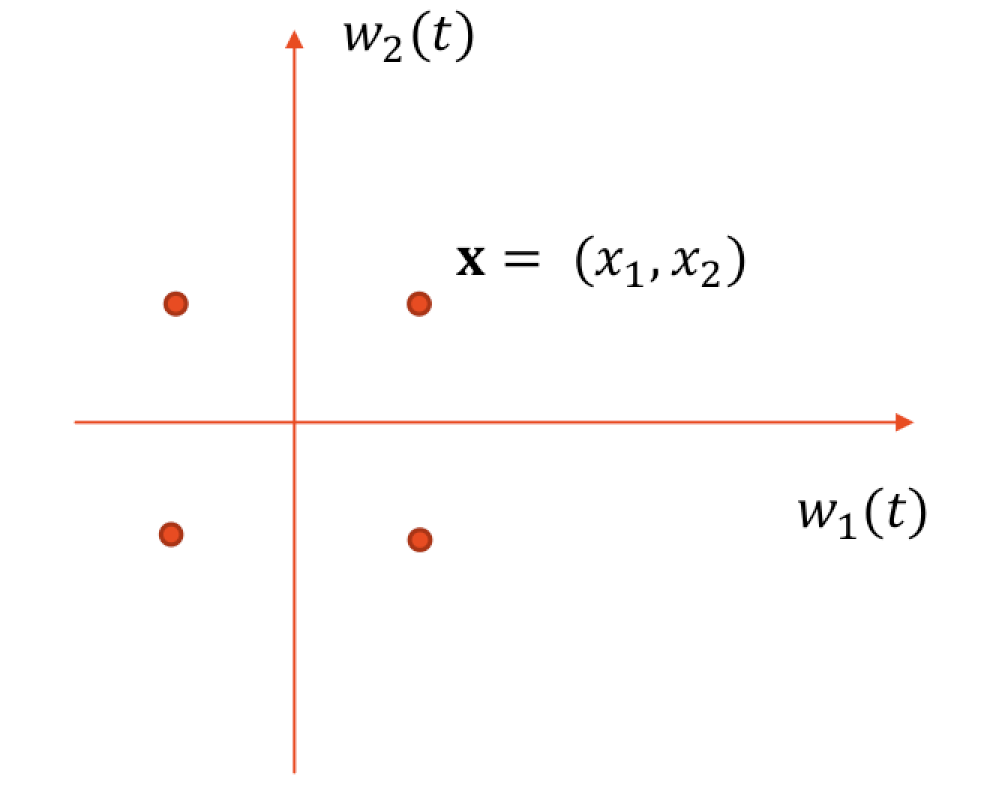
\includegraphics[width=0.5\textwidth]{img/wireless/iq representation.png}
        \caption{Some points that represent some signals in the I/Q representation}
        \label{fig:Complex Plane}
      \end{figure}
    \end{subsubsection}
  \end{subsection}
  \begin{subsection}{Fourier Analysis}
    Lets consider a signal with base the complex exponential functions 
    \begin{equation}
      e^{j2\pi \frac{n}{T} t} = cos(2\pi \frac{n}{T} t) + j sin(2\pi \frac{n}{T} t)
      \label{euler formula}
    \end{equation}
    It is actually characterized by a frequency $f_n = \frac{n}{T}$, where T is the period of the
    signal. The higher the frequency, the more oscillations we will have in the same time interval.
    In this function they have both the same frequency.\\

    We can use that function as a basis to decompose a signal, again. This is because it is 
    possible to generate an infinite set of functions
    \begin{equation}
      w_n(t) = \frac{1}{\sqrt{T}} e^{j\frac{2\pi}{T} nt} 
    \end{equation}
    with $-T/2 \leq t \leq T/2$, each associated with a frequency.
    That can be used ad a complete basis for all the signals limited in $[-T/2, T/2]$ or periodic.\\
    For example, we can write a signal as a linear combination of these functions:
    \begin{equation}
      x(t) = \frac{1}{\sqrt{T}} \sum_{n=-\infty}^{\infty} c_n e^{j\frac{2\pi}{T} nt}
      \label{Fourier Series}
    \end{equation}
    where $c_n$ are the coefficients of the linear combination $c_n = \langle x(t), w_n(t) \rangle$.\\
    Each one of those coefficients is a measure of how much each frequency $f_n$, of the $n$-th
    sinusoid(the shape of equation \ref{euler formula}) is present in the signal $x(t)$.\\
    \begin{figure}[h]
      \centering
      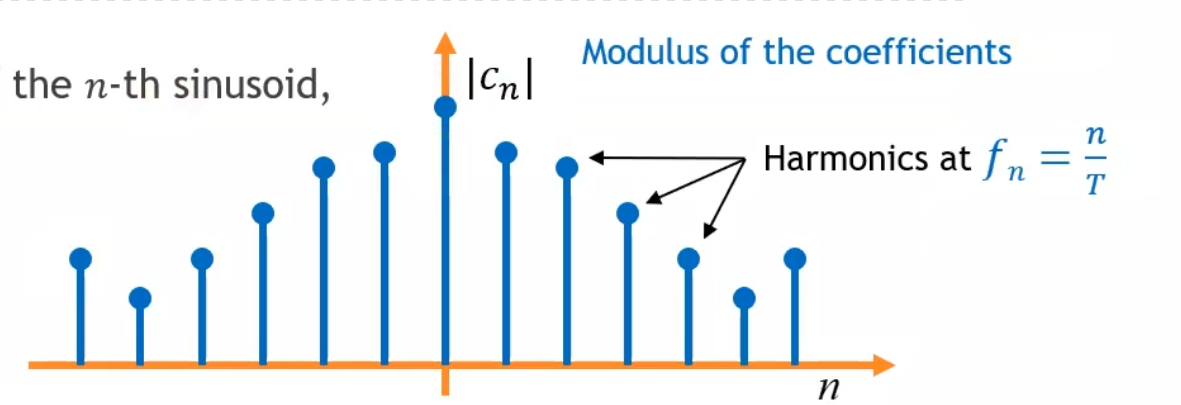
\includegraphics[width=0.7\textwidth]{img/wireless/euler plot.png}
      \caption{Plot of the coefficients of equation \ref{Fourier Series}}
      \label{fig:Fourier Analysis}
    \end{figure}
    Lets now take a look at picture \ref{fig:Fourier Analysis}. We can see that the coefficients
    are higher when the frequence is very small, so the signal \ref{Fourier Series} is mostly
    composed by large components of low frequency.\\
    This whole concept is called \textbf{Fourier Analysis}, or frequency analysis, which allows
    to decompose a signal into a set of frequencies.
    \begin{boxH}
    TLDR: I can build a signal trough a combination of frequency components. \\
    The coefficients of this frequency components are the measure of how much each frequency is 
    present in the signal.
    \end{boxH}
    Now we just need to expand it to any signal and any frequency( a continuous frequency domain).
    By doing so we can derive the definition of the \textbf{Fourier Transform} of a signal $x(t)$:
    \begin{equation}
      X(f) = \int_{-\infty}^{\infty} x(t) e^{-j2\pi ft} dt
      \label{Fourier Transform}
    \end{equation}
    where $X(f)$ is the Fourier Transform of the signal $x(t)$, and $f$ is the frequency.\\
    The Fourier transform is equivalent to a scalar product between the signal and the complex
    exponential function at a given frequency $f$. This means that each of the values of the
    Fourier Transform is a measure of how much the frequency $f$ is present in the signal $x(t)$.\\
    Furthermore, trough the inverse of equation \ref{Fourier Transform}
    \begin{equation}
      x(t) = \int_{-\infty}^{\infty} X(f) e^{j2\pi ft} df
      \label{Inverse Fourier Transform}
    \end{equation}
    we can write again a signal $x(t)$ as a linear combination of the complex exponential functions
    , which represents the frequency components of the signal, weighted by the Fourier Transform.\\
      
    \begin{boxH}
      The Fourier Transform $X(F)$ indicates the "weight" of each frequency component( sinusoidal
      component at a given frequency $f$) in the signal $x(t)$.\\
      The inverse Fourier Transform $x(t)$ tells us we can decompose any signal into frequency 
      components( sinusoidal components at a given frequency $f$).
    \end{boxH}
    
    \begin{figure}[h]
      \centering
      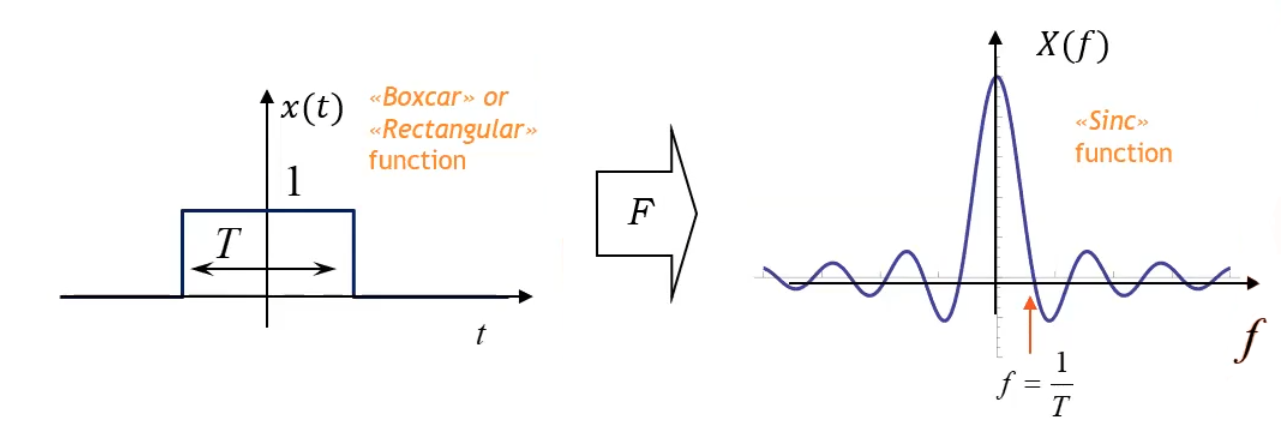
\includegraphics[width=0.9\textwidth]{img/wireless/fourier square function.png}
      \caption{Fourier Transform of a square function}
      \label{fig:Fourier Transform}
    \end{figure}

    With that in mind, take a look at figure \ref{fig:Fourier Transform}. It represents a rectangular
    signal (a signal that is 1 for a certain time, and 0 for the rest of the time), and its Fourier
    Transform, which tells us the frequency components of the signal.\\
    From that, we can see that the Fourier Transform is mostly composed by low frequency components,
    because values closer to zero are higher. That is because in the constant part of the signal
    has a sinusoidal component that constant.

    \begin{boxH}
      To wrap it up, for each signal we have a \textbf{spectral representation}. And for each operation
      over a signal, there are equivalents effects in the frequency domain.\\
      Furthermore, a signal that has finite duration in time, has a infinite support in the frequency
      domain.
    \end{boxH}
  \end{subsection}
  \begin{subsection}{Bandwidth}
    The bandwidth is the \textbf{interval of frequencies} that a signal occupies.\\
    If we consider a signal $x(t)$, we can define the bandwidth as the interval of frequencies
    where the Fourier Transform $X(f)$ is different from zero. \\ 
    Signals have often infinite support over the frequency domain over a finite duration, but many 
    of them are characterized by a quasi-null(finite) spectrum outside a certain interval of 
    frequencies( the main lobes of the spectrum).\\
    For this reason, we usually consider the bandwidth around half of the frequency spectrum of the
    signal, as shown in figure \ref{fig:Bandwidth}(for example 3dB bandwidth, or half power 
    bandwidth).\\
    \begin{figure}[h]
      \centering
      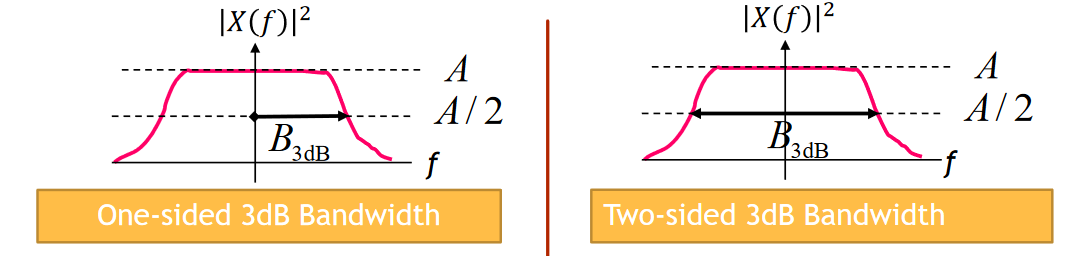
\includegraphics[width=0.8\textwidth]{img/wireless/bandwidth.png}
      \caption{Bandwidth of a signal}
      \label{fig:Bandwidth}
    \end{figure}
    \begin{subsubsection}{Bandwidth in linear systems}
      A \textbf{system} is a set of operations applied to signals.\\
      The relationship between the bandwidth of the input signal and the bandwidth of a system is
      usually very important. In fact, when a system is used to pass or remove particular 
      frequencies of a signal, it can be regarded as a system.\\
      We can associate a bandwidth to a system, specifically a \textbf{linear-time invariant} system,
      with a \textbf{frequency response} $H(f)$.This mean that we can associate a bandwidth to a
      system, making us able to compute a new bandwidth $Y(f)$ by combining together the bandwidth 
      $X(f)$ of the input signal and the frequency response $H(f)$ of the system($Y(f) = X(f)H(f)$
      in formulas).\\
      This concept can be represented graphically very easily, like in figure 
      \ref{fig:Bandwidth System}. If the result of the combination of the input signal and the
      sequence of operation of the system is a signal with a bandwidth $Y(f)$. If the bandwidth of 
      the linear system is larger than the origin signal, the signal pass trough smoothly($Y(f) \approx X(f)$).\\
      However, if the bandwidth of the signal is larger than the bandwidth of the system, the signal
      will be cutted off($Y(f) \ne H(f)$).\\

      \begin{figure}[h]
        \centering
        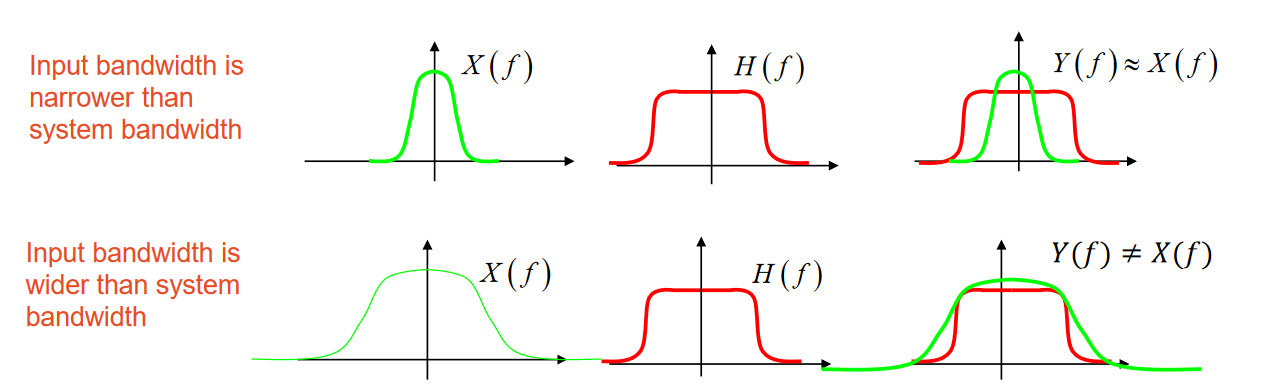
\includegraphics[width=0.8\textwidth]{img/wireless/bandwidth system.png}
        \caption{Bandwidth of a system}
        \label{fig:Bandwidth System}
      \end{figure}
    \end{subsubsection}
  \end{subsection}

  \begin{subsection}{Filters}
    A filter is a system used to model desired and undesired effects over a signal.\\
    It is usually used to remove undesired frequency components from a signal, but overall can be
    used to:
    \begin{itemize}
      \item share the wireless medium
      \item model the spectrum of a signal over the channel
      \item mitigate undesired effects over a signal trough equalizers
    \end{itemize}
    \end{subsection}
    \begin{subsection}{Signal modulation}
      Signal modulation is the process of multiplying a signal by a sinusoidal function, resulting
      in a \textbf{frequency shift}.
      \begin{equation}
        y(t) = x(t) \cdot cos(2\pi f_0 t)
      \end{equation}
      This is possible because
      \begin{equation}
        F(x(t) \cdot cos(2\pi f_0 t)) = \frac{1}{2}[X(f-f_0) + X(f+f_0)]
      \end{equation}
      where $X$ is the frequency domain representation.\\ 
      \begin{figure}[h]
        \centering
        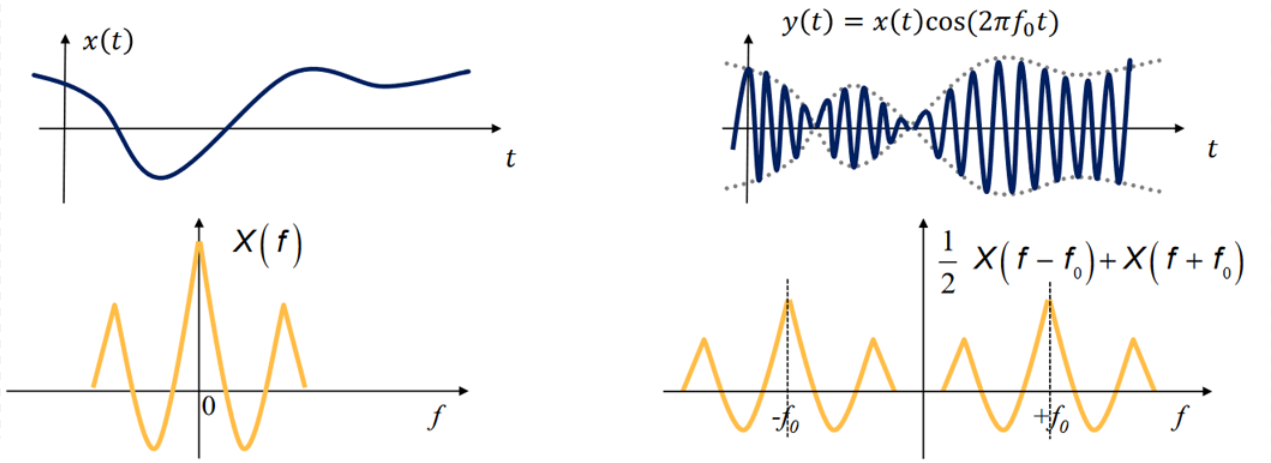
\includegraphics[width=0.8\textwidth]{img/wireless/signal modulation.png}
        \caption{Graphical representation of the modulation}
        \label{fig:Modulation}
      \end{figure}
      We can see that as a result of the modulation, the spectrum of the signal is shifted around
      the frequency $f_0$, as shown in figure \ref{fig:Modulation}.\\

    \end{subsection}
    \begin{subsection}{Signal demodulation}
      When modulating a signal, we alter it a bit, centering it around the frequency $f_0$, shifting
      the spectrum of the signal. The effect of this operation is not trivial.\\
      To recover the original signal, we need to multiply the modulated signal by a sinusoidal
      function at the same frequency $f_0$ as the one used for the modulation. This allows us to
      shift the spectrum back to the original position.\\
      This operation is called \textbf{demodulation}.\\
      A given modulated signal $Y(f)$
      \begin{equation}
        Y(f) = \frac{A}{2}[X(f-f_0) + X(f+f_0)]
      \end{equation}
      shown in figure \ref{fig:Demodulation1}
      \begin{figure}[h]
        \centering
        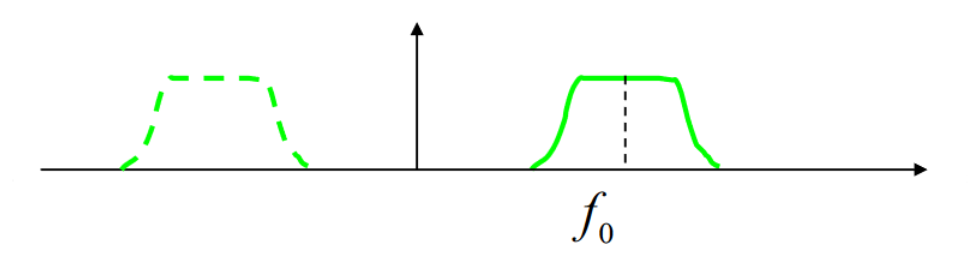
\includegraphics[width=0.8\textwidth]{img/wireless/demodulation1.png}
        \caption{A modulated signal at frequency $f_0$}
        \label{fig:Demodulation1}
      \end{figure}
      can be demodulated by multiplying it by the same sinusoidal function used for the modulation
      \begin{equation}
        Y'(f) = Y(f) \cdot cos(2\pi f_0 t)= \frac{A}{2}X(f)+\frac{A}{4}[X(f-2f_0)+X(f+2f_0)]
      \end{equation}
      shown in figure \ref{fig:Demodulation2}\\
      \begin{figure}[h]
        \centering
        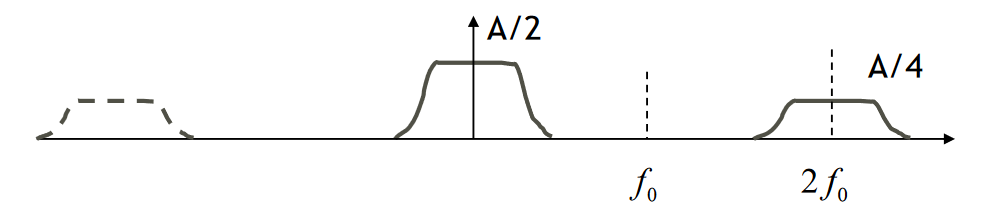
\includegraphics[width=0.8\textwidth]{img/wireless/demodulation2.png}
        \caption{A demodulated signal at frequency $f_0$}
        \label{fig:Demodulation2}
      \end{figure}
      This doesn't allow us to recover the original spectrum of the signal.
      That's why we need to use a \textbf{low-pass filter} to remove the frequency components at
      $2f_0$ and its symmetrical counterpart, as shown in figure \ref{fig:Demodulation3}.\\
      \begin{figure}[h]
        \centering
        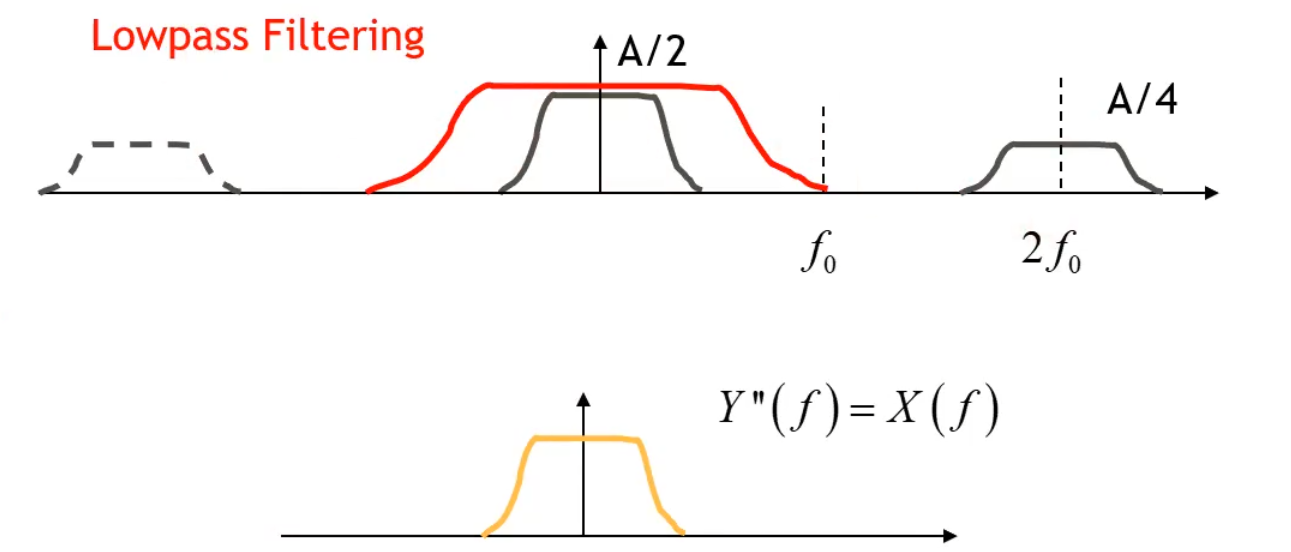
\includegraphics[width=0.8\textwidth]{img/wireless/demodulation3.png}
        \caption{A demodulated signal at frequency $f_0$ after a low-pass filter}
        \label{fig:Demodulation3}
      \end{figure}

    \end{subsection}
    \begin{subsection}{Frequency Multiplexing(FDM)}
      \label{subsec:FDM}
      Modulation and demodulation allows multiple wireless communication systems to coexist at different
      frequencies.\\
      For example, if i want to transmit different signals with overlapping bandwidths, i can simply
      modulate each signal at a different frequency, and then transmit them all together, as shown in
      figure \ref{fig:FDM}.\\
      Once received the signal, each of those signals can be demodulated by multiplying it by the 
      same function at the same frequency used for the modulation.\\
      \begin{figure}[h]
        \centering
        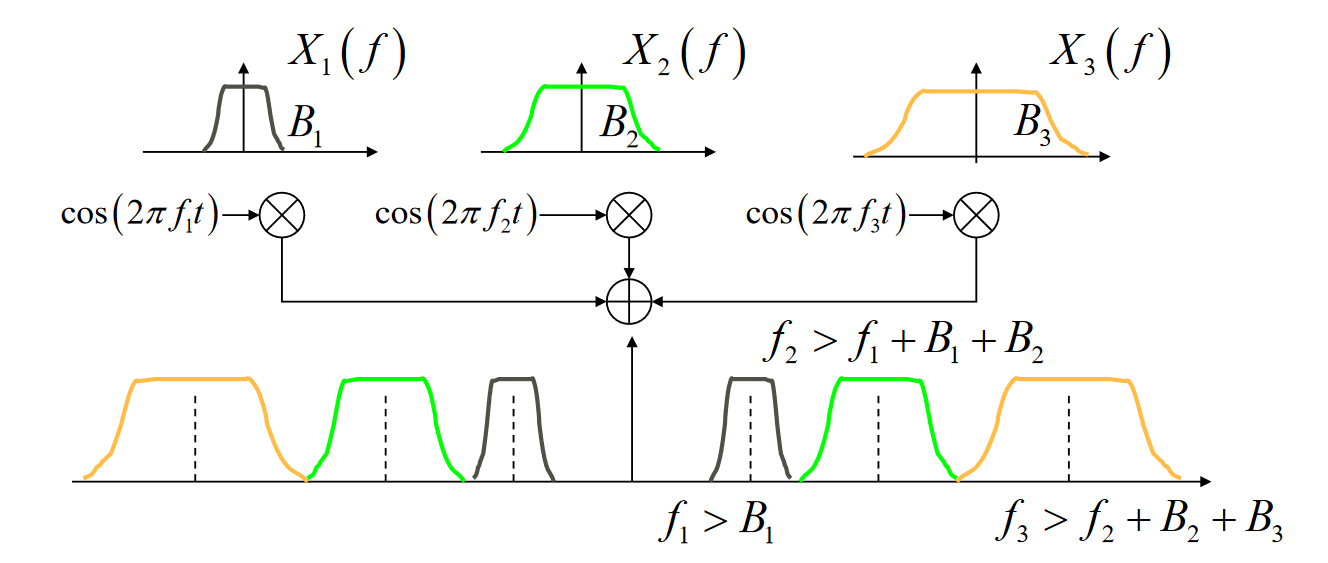
\includegraphics[width=0.9\textwidth]{img/wireless/FDM.png}
        \caption{Frequency Multiplexing}
        \label{fig:FDM}
      \end{figure}
    \end{subsection}
    \begin{subsection}{Analog-to-Digital Conversion}
      We can now deal with signals, but we still have to convey information.\\
      The informations can be both \textbf{analog} or \textbf{digital}. Usually, transmitting digital
      information is ideal, because it has some advantages, such as error detection and correction,
      and the possibility to compress the information. On the other hand, we still have to convert
      digital information to analog information to be transmitted over the channel, after converting
      it to a stream of bits.\\
      Once the signal is received, it has to be converted back to digital information. To do so,
      first of all the signal it has to be sampled, which can be a lossless operation if the sampling
      frequency is high enough.\\
      After the sampling, the sample has to be quantized, which is the process of converting the
      amplitude of the sample to a digital value at discrete times( because it is a continuous
      time function, which would require an infinite number of digits to represent). Each of those 
      values is associated with a given amplitude, which is associated to a number, which 
      eventually is converted into binary digits. We can also observe that quantization is a lossy
      operation by definition.\\
      At the end of the fair, a sequence of bits is obtained, which can be transmitted over the
      channel.\\
      \begin{figure}[h]
        \centering
        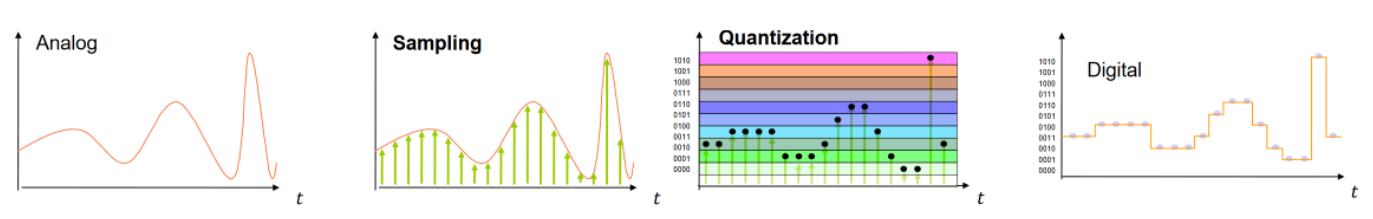
\includegraphics[width=\textwidth]{img/wireless/analog to digital.png}
        \caption{Analog-to-Digital Conversion}
        \label{fig:ADC}
      \end{figure}
      \begin{subsubsection}{Sampling theorem}
        As previously stated, the sampling operation can be lossless if the sampling frequency is
        high enough. This is because of the \textbf{Nyquist sampling theorem}, which states
        that a signal can be perfectly reconstructed from its samples if the sampling frequency is
        at least twice the bandwidth of the signal.\\
        \begin{equation}
          f_c=\frac{1}{T_c}>2B\to T_c<\frac{1}{2B}
        \end{equation}
        where $f_c$ is the sampling frequency, $T_c$ is the sampling period, and $B$ is the bandwidth.
        \end{subsubsection}
    \end{subsection}
\end{section}

\begin{section}{Signal Transmission and Reception}
  Now that we know how a signal can be represented and processed, we can start to think how each 
  component of a communication system can be designed.\\
  \begin{subsection}{Digital Modulations}
    The end goal is to have a reliable communication system, which can transmit and receive
    information. As such, a important design choose is the signal waveform to transmit.\\
    The \textbf{modulator} is the component of the system that takes the digital information and 
    modulates it to a signal that can be transmitted over the channel. The demodulator component 
    just does the opposite, taking the signal and converting it back to digital information.\\

    \begin{boxH}
      \textbf{Modulation} is the process of varying one or more properties of a periodic waveform, called
      the \textbf{carrier}, with a modulating signal that typically contains information to be
      transmitted.
    \end{boxH}
    This process is necessary not only to cope with the analog channel, but also to allow multiple
    communication systems( which means different signals) to coexist in the same channel.\\

    Generally, digital and analog modulations resort to basic modulation types:
    \begin{itemize}
      \item \textbf{Amplitude Modulation(AM)}, which changes the amplitude of the carrier
      \item \textbf{Frequency Modulation(FM)}, which changes the frequency of the carrier
      \item \textbf{Phase Modulation(PM)}, which changes the phase of the carrier
    \end{itemize}

    This kind of modulation is necessary to convey information to the receiver, assigning to each
    possible value of the information signal a different amplitude, frequency or phase.
    \begin{subsubsection}{Amplitude Modulation(AM)}
      The amplitude modulation is the simplest form of modulation.\\
      The amplitude of an high-carrier signal(like a cosine signal) is varied according to the 
      instantaneous amplitude of the modulating message signal $m(t)$.\\
    \end{subsubsection}
    \begin{subsubsection}{Frequency Modulation(FM)}
      In frequency modulation, the frequency of the carrier signal is varied by the modulating
      signal $m(t)$, while the amplitude of the carrier signal is kept constant.\\
      This means that the as the amplitude of the information signal varies, the carrier frequency
      varies as well. For example, if the amplitude of the information signal increases, the
      frequency of the carrier signal increases as well.\\
      \begin{figure}[h]
        \centering
        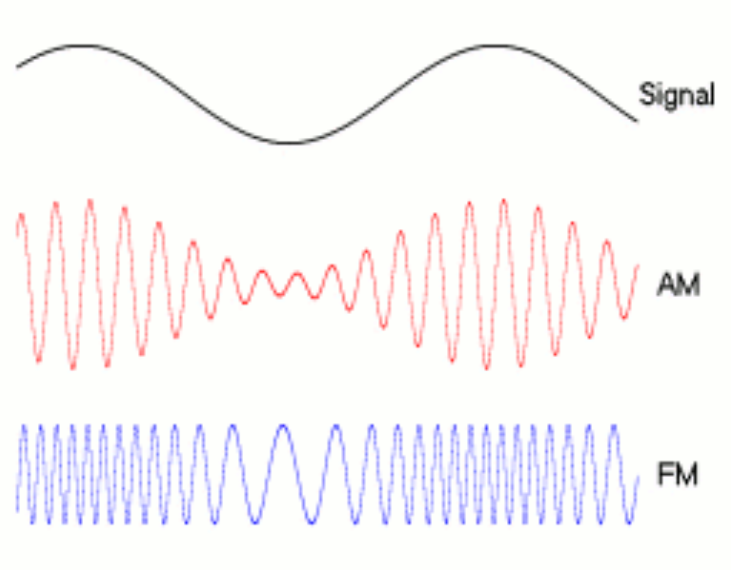
\includegraphics[width=0.4\textwidth]{img/wireless/AM-FM.png}
        \caption{An example of a signal modulated in amplitude and frequency}
        \label{fig:AM-FM}
      \end{figure}
    \end{subsubsection}
    \begin{subsubsection}{Phase Modulation(PM)}
      Phase modulation is a form of modulation that encodes the signal $m(t)$ as a variation in the
      instantaneous phase of a carrier wave.\\
      This means that the phase of a carrier is modulated to follow the changing in the signal 
      amplitude of the message signal.\\

      The peak amplitude and the frequency of the carrier signal are maintained constant, but as 
      the amplitude of the message signal changes, the phase of the carrier changes 
      correspondingly.\\
      \begin{figure}[h]
        \centering
        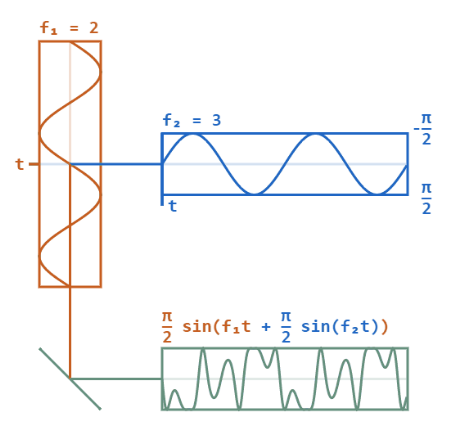
\includegraphics[width=0.5\textwidth]{img/wireless/PM.png}
        \caption{An example of a signal modulated in phase. The modulating wave(in blue) is modulating
          the phase of the carrier wave(in red), resulting in the PM signal(in green)}
        \label{fig:PM}
      \end{figure}
    \end{subsubsection}
    \begin{subsubsection}{Analog-to-Digital modulations}
      Even if the world has turned to digital, transmitted signals are analog.\\
      This means that the digital information has to be converted to an analog signal to be
      transmitted over the channel. But the receiver still need to understand the digital information
      from the received signal.\\
      To be sure that the information can be recovered, the signal has to be modulated in a way that
      the receiver can understand the digital information. This can be done by varying some proprieties
      of the carrier signal, such as the amplitude, the frequency, or the phase, to represent the
      digital information.\\
      \begin{figure}[h]
        \centering
        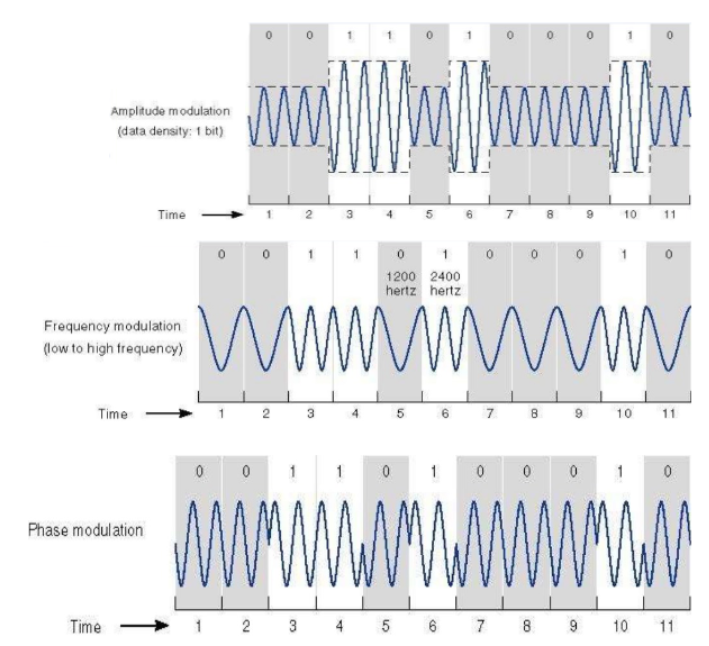
\includegraphics[width=0.5\textwidth]{img/wireless/modulation encoding.png}
        \caption{Some example of modulations used to represent digital information. From top to bottom:
          Amplitude Shift Keying, Frequency Shift Keying, Phase Shift Keying}
        \label{fig:DigitalModulation}
      \end{figure}
      The carrier signal is used to modulate the digital information, so we can distinguish between
      different kinds of signals:
      \begin{itemize}
        \item the \textbf{the baseband signal}, which is the unmodulated signal, whose spectrum is
          centered around zero frequency
        \item the \textbf{passband signal}, which is the modulated signal, whose spectrum is centered
          around the carrier frequency
      \end{itemize}
      The baseband signal can be converted to a passband signal by multiplying it by a carrier signal
      with the desired frequency.\\
    \end{subsubsection}
    \begin{subsubsection}{Baseband Signals}
      The simplest kind of digital modulation is the \textbf{Pulse Amplitude Modulation(PAM)}, which
      is a form of modulation where the message signal is encoded in the amplitude of a series of
      signal pulses.\\
      For example, if we have a binary signal, we can encode the 0 as a low amplitude pulse $-A$, and the
      1 as a high amplitude pulse $A$. The simplest pulse is a rectangular one, but other kind of 
      pulses can be used.\\
      If we have a binary PAM(2-PAM), the signal can be represented as:
      \begin{itemize}
        \item $s(t)=g(t) \to "1"$
        \item $s(t)=-g(t) \to "0"$
      \end{itemize}
      where $g(t)$ is the basic pulse shape.\\
      \begin{figure}[h]
        \centering
        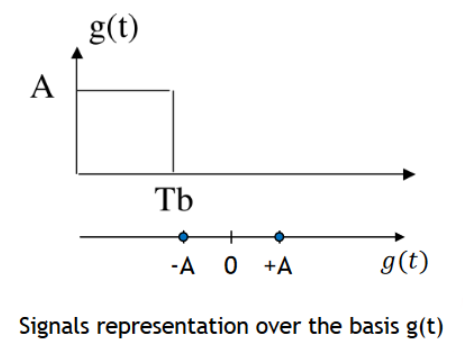
\includegraphics[width=0.4\textwidth]{img/wireless/2-PAM.png}
        \caption{An example of a 2-PAM signal representation}
        \label{fig:PAM}
      \end{figure}
    \end{subsubsection}
    \begin{subsubsection}{M-ary PAM}
      WA 2-PAM signal can only represent 1 bit of information. To represent more bits, we can use
      M-ary PAM, where M is the number of different symbols that can be represented, while still
      using the same base signal.\\
      For example, a 4-PAM signal can represent 2 bits of information by defining 4 levels of
      amplitude, and can be represented as:
      \begin{itemize}
        \item $s(t)=3g(t) \to "00"$
        \item $s(t)=g(t) \to "01"$
        \item $s(t)=-g(t) \to "10"$
        \item $s(t)=-3g(t) \to "11"$
      \end{itemize}
      This definition can be generalized to:
      \begin{equation}
        s_i(t)=A_i g(t),\quad i=1,2,\dots,M
      \end{equation}
      allowing to represent $log_2(M)$ bits of information.\\
      \begin{figure}[h]
        \centering
        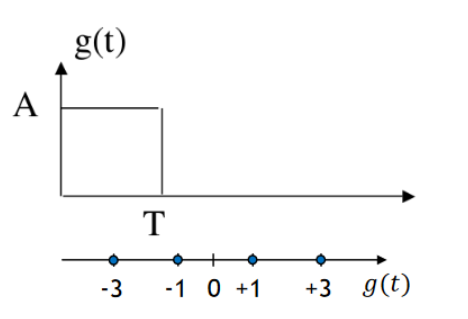
\includegraphics[width=0.4\textwidth]{img/wireless/M-PAM.png}
        \caption{An example of a 4-PAM signal representation}
        \label{fig:4-PAM}
      \end{figure}
    \end{subsubsection}
    \begin{subsubsection}{Gray Coding}
      When using M-ary PAM, it is important to use a coding that minimizes the error probability.
      After all, Symbols that are close to each other in the signal space are more likely to be 
      confused, so the choice of the number of symbols and the distance between them is 
      important.\\
      \begin{boxH}
        \textbf{Gray coding} is a strategy to \textbf{mapping bits to symbols} that minimizes the
        probability of error.
      \end{boxH}
      Gray coding achieves 1-bit error correction, meaning that if a error is to occur, it will only
      affect 1 bit of the message with a high probability.\\
      \begin{figure}[h]
        \centering
        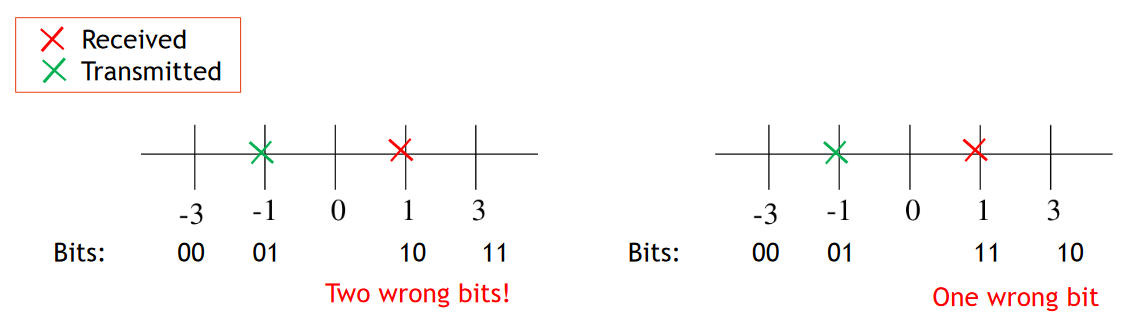
\includegraphics[width=0.8\textwidth]{img/wireless/gray coding.png}
        \caption{An example of a 4-PAM signal representation using Gray coding}
        \label{fig:GrayCode}
      \end{figure}
    \end{subsubsection}
    \begin{subsubsection}{Energy per bit}
      A measure of the energy efficiency of a modulation can be obtained by calculating the average
      energy per bit.\\
      The energy per bit can be defined as 
      \begin{equation}
        E_b=\frac{E_s}{log_2(M)}
      \end{equation}
      where $E_s$ is the energy of the signal, and $M$ is the number of symbols, or in a more
      discursive way, the average energy per symbol divided by the number of bits carried by 
      each symbol.\\
      This concept can also be visualized graphically, as the distance of a symbol from the origin
      in the signal space(as in figure \ref{fig:4-PAM}), because it is proportional to 
      energy of the symbol.\\

      The energy per symbol can be calculated as
      \begin{equation}
        E_s=\int_{0}^{T} (S_m(t))^2 dt= (A_m)^2 \int_{0}^{T} (g(t))^2 dt= (A_m)^2 E_g
      \end{equation}
      where $S_m(t)$ is the modulated signal, $A_m$ is the amplitude of the modulated signal, $g(t)$
      is the base pulse, and $E_g$ is the energy of the base pulse.\\

      For example, the average energy per symbol for the 4-PAM of figure \ref{fig:4-PAM} is
      \begin{equation}
        E_s=\frac{3^2T+1^2T+1^2T+3^2T}{4}=5T
      \end{equation}
      Generally, the larger the energy, the larger the distance between the symbols, and the lower
      the probability of error(mistaking one symbol for another). On the other hand, the larger the
      number of symbols over the same bandwidth, the less energy is required to transmit each bit(
      because each symbol is closer and carries more bits).\\
    \end{subsubsection}

    \begin{subsubsection}{Bandpass Signals}
      As previously stated, to transmit a baseband signal $s(t)$ trough a passband channel, we 
      have to modulate it at a certain frequency $f_c$, by multiplying it by a sinusoidal carrier
      signal with that frequency, otherwise it will be centered around zero frequency.\\
    \end{subsubsection}

    \begin{subsubsection}{Bandwidth Occupancy and efficiency}
      The shape of a signal determine the bandwidth it occupies.\\
      For example, a rectangular function has a pulse spectrum that is a sinc function, shown in
      figure \ref{fig:rectangular pulse spectrum}, which has a symbol rate of $1/T$(the amount of 
      symbols per second).

      \begin{figure}[h]
        \centering
        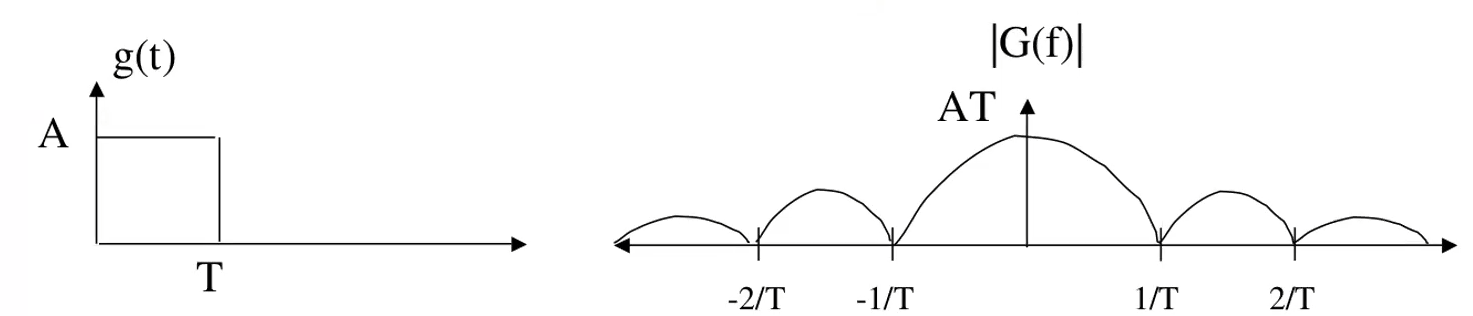
\includegraphics[width=0.6\textwidth]{img/wireless/rectangular pulse spectrum.png}
        \caption{The spectrum of a rectangular pulse}
        \label{fig:rectangular pulse spectrum}
      \end{figure}

      Usually, a smaller base pulse will require less energy to transmit, but will occupy more
      bandwidth. A longer basic pulse will require more energy to transmit, but will occupy less
      bandwidth and have a lower bit rate.\\

      With that in mind, ideally, we would like to choose a pulse shape $g(t)$ that minimizes the
      bandwidth occupancy, putting more energy in the lower frequencies, resulting in a smaller
      bandwidth.\\

      For a pulse duration $T$, we can define the \textbf{symbol rate} as $R_s=1/T$, and the
      \textbf{bit rate} as $R_b=R_s log_2(M)$(recall that $log_2(M)$ is the number of bits per
      symbol).\\
      The bit rate efficiency can be defined as
      \begin{equation}
        \eta=\frac{R_b}{BW}=\frac{log_2(M)}{T} \times (\frac{T}{2})=\frac{log_2(M)}{2}\text{bps/Hz}
      \end{equation}
      where $BW$ is the two sided bandwidth of the signal $BW=2R_2=\frac{2}{T}$.\\
      As we can see, the bit rate efficiency is proportional to the number of bits per symbol
      ($\eta \propto M$) and inversely proportional to the pulse duration. The duration of the 
      pulse is uninfluent.\\

      We can also consider some examples:
      \begin{itemize}
        \item 2-PAM: $\eta=\frac{1}{2}\text{bps/Hz}$
        \item 4-PAM: $\eta=\frac{2}{2}\text{bps/Hz}$
        \item 8-PAM: $\eta=\frac{3}{2}\text{bps/Hz}$
      \end{itemize}
      As we can see, the bandwidth efficiency increases with the number of bits per symbol, because
      we are fitting more bits in the same bandwidth.\\
      This also means that our signal will be more susceptible to noise, because the symbols are
      closer to each other, making it easier to mistake one for another. To reduce the probability
      of errors, we have to increase the energy per symbol, which will increase the bandwidth
      occupancy. For those reasons, there's a trade-off between bandwidth occupancy and energy
      efficiency.\\

      \begin{figure}[h]
        \centering
        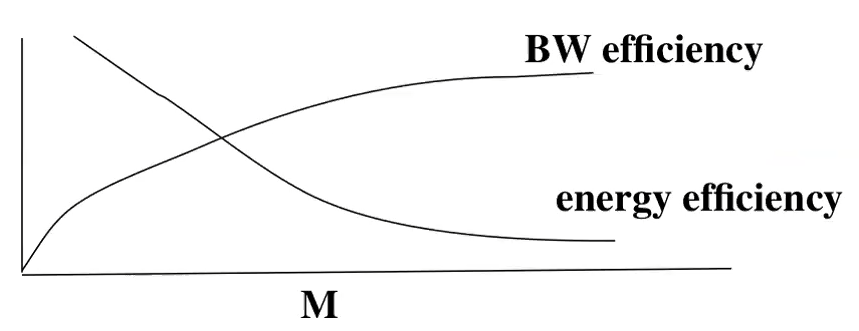
\includegraphics[width=0.6\textwidth]{img/wireless/energy efficiency vs bandwidth occupancy.png}
        \caption{Trade-off between energy efficiency and bandwidth occupancy}
        \label{fig:energy efficiency vs bandwidth occupancy}
      \end{figure}

    \end{subsubsection}
    \begin{subsubsection}{Two-dimensional Modulation}
      As introduced in subsection \ref{sub:IQ representation}, signals can be represented over two 
      orthonormal basis. This means that we can represent a signal in a 2D plane, with the
      in-phase and quadrature components as the x and y axis.\\
      This representation allows to represent the set of signals $s_i$(also called \textit{constellation}
      over two orthonormal basis. A large constellation will allow to represent more bits per symbol,
      which results in a higher bit rate(bandwidth efficiency), but also a higher probability of 
      error.\\

      \begin{boxH}
        The shape of the constellation is important, because it can be used to minimize the probability
        of error, by choosing a constellation that minimizes the distance between the symbols.
      \end{boxH}
      \begin{figure}[h]
        \centering
        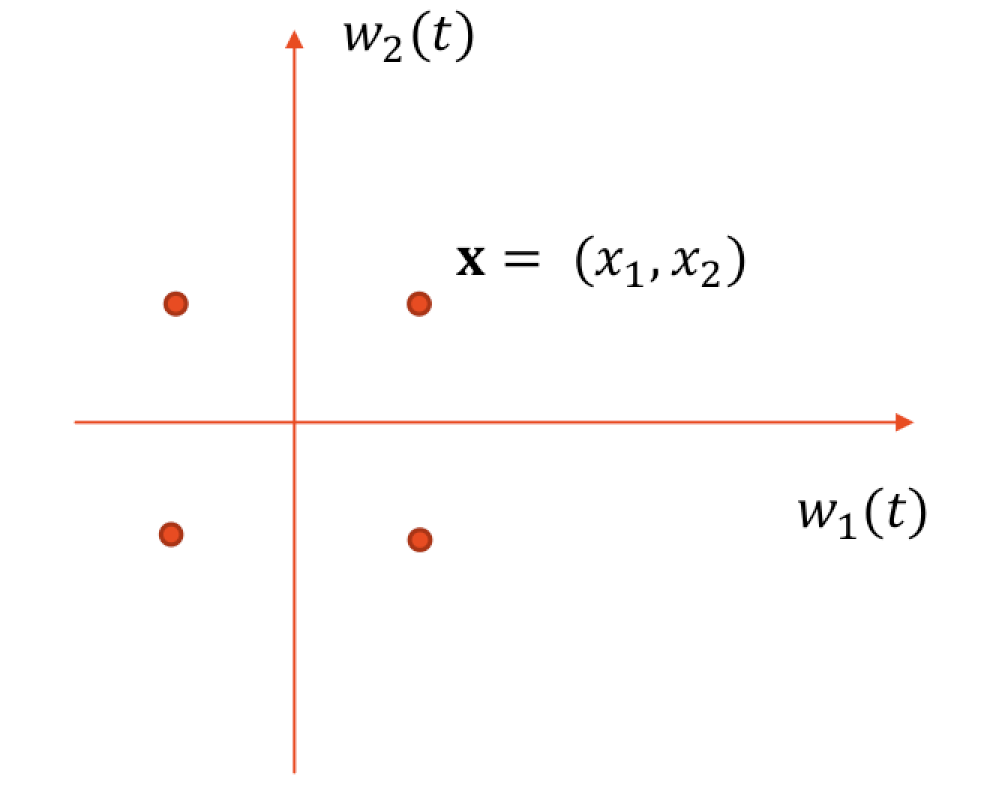
\includegraphics[width=0.5\textwidth]{img/wireless/iq representation.png}
        \caption{A constellation of 4-PAM signals}
      \end{figure}
      Furthermore, there are some common constellations that are used in practice, such as:
      \begin{itemize}
        \item \textbf{QAM}: Quadrature Amplitude Modulation, which is a PAM signal over two
          dimensions.
        \item \textbf{PSK}: Phase Shift Keying, which is a PAM signal over the phase of a signal, 
          meaning that the amplitude is constant.
      \end{itemize}
    \end{subsubsection}

    \begin{subsubsection}{M-QAM}
      \begin{boxH}
        M-QAM is a modulation that represents the signal as the sum of two signals, represented over
        two orthonormal basis. This means that we can have $M$ symbols to modulate out signal.
      \end{boxH}
      Thus, we can represent $\sqrt{M}$ symbols over each axis, and the total number of
      symbols is $M$.\\
      This means that a symbol, represented over two orthonormal basis, can be described as 
      \begin{equation*}
        S_m=(A^x_m,A^y_m),A^x_m,A^y_m \in \{+/-1,\dots,+/-(\sqrt{M}-1)\}
      \end{equation*}
      for example:
      \begin{itemize}
        \item 4-QAM: $A^x_m,A^y_m \in \{+/-1\}$
        \item 16-QAM: $A^x_m,A^y_m \in \{+/-1,+/-3\}$
      \end{itemize}

      \begin{figure}[h]
        \centering
        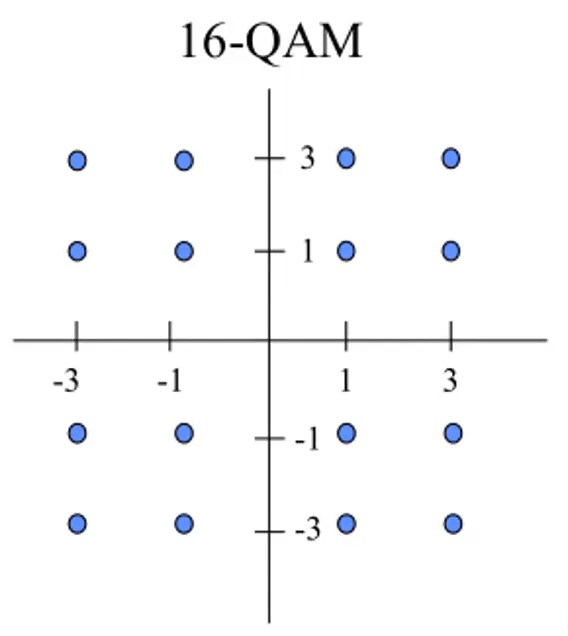
\includegraphics[width=0.4\textwidth]{img/wireless/16 QAM.png}
        \caption{A 16-QAM constellation}
      \end{figure}

      We recall that with QAM, the amplitude and phase of the signal are modulated. This means that
      by using the same pulse shape $g(t)$, the bandwidth efficiency is the same of a M-PAM, because
      the number of bits per symbol is the same, but with a larger energy efficiency, thanks to the
      presence of another dimension.\\

      By entering in the details, the in-phase and quadrature components of the signal are modulated
      by multiplying the components to orthogonal carriers, meaning that we can separate them 
      easily afterwards. This operation also transform the signal to a bandpass one.\\
      This is accomplished by multiplying the $A^x$ component by Cosine and the $A^y$ component by
      Sine, and then summing the two signals.\\

      The transmitted signal can thus be described as
      \begin{equation}
        U_m(t)= A_m^xg(t)cos(2\pi f_c t)+A_m^yg(t)sin(2\pi f_c t),m=1,\dots,M
      \end{equation}
      or in a more discursive way, each component of the signal is the amplitude value over one axis
      multiplied by the base pulse(the basis), and then multiplied by a carrier signal at a 
      given frequency.\\
    \end{subsubsection}
    \begin{subsubsection}{M-QAM modulation and demodulation}
      The general schema of M-QAM modulation is shown in figure \ref{fig:MQAM modulation}.\\
      We receive in input a series of bits, which are associated with the corresponding symbols, 
      one for each axis. The symbols used to modulate the pulse signal are then multiplied by the
      pulse shape, and then by the carrier signal. The two signals are then summed and transmitted.\\

      \begin{figure}[h]
        \centering
        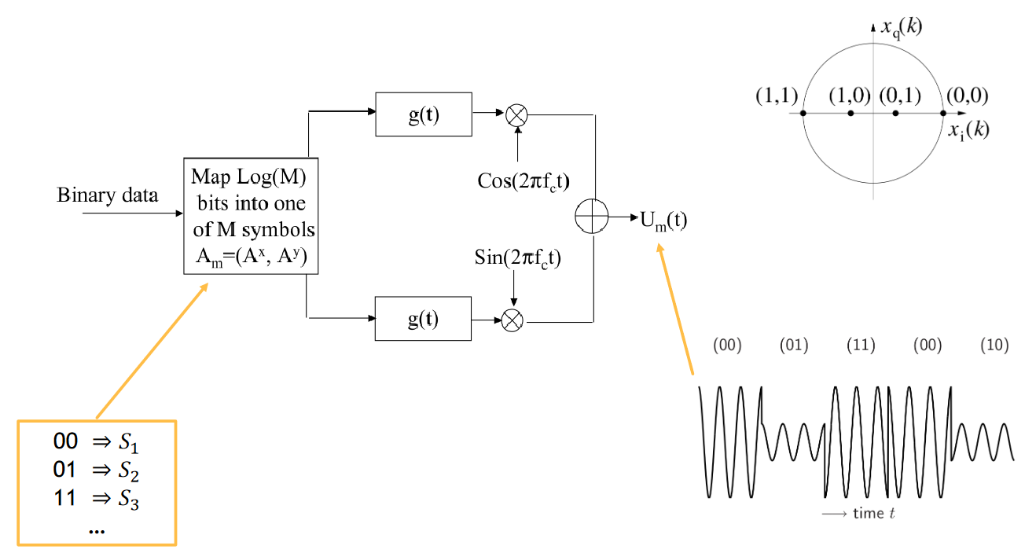
\includegraphics[width=0.7\textwidth]{img/wireless/MQAM modulation.png}
        \caption{General schema of M-QAM modulation}
        \label{fig:MQAM modulation}
      \end{figure}

      As for what concerns the demodulation, we want to understand correctly the symbols that we
      receive, so we don't really care about the carrier signal. 
      We can notice that the sin and cosine components of the signal are orthogonal, meaning that
      we are able to separate them easily: the cosine component disappears after filtering when multiplied
      by the sine component, and viceversa.\\
      \begin{figure}[h]
        \centering
        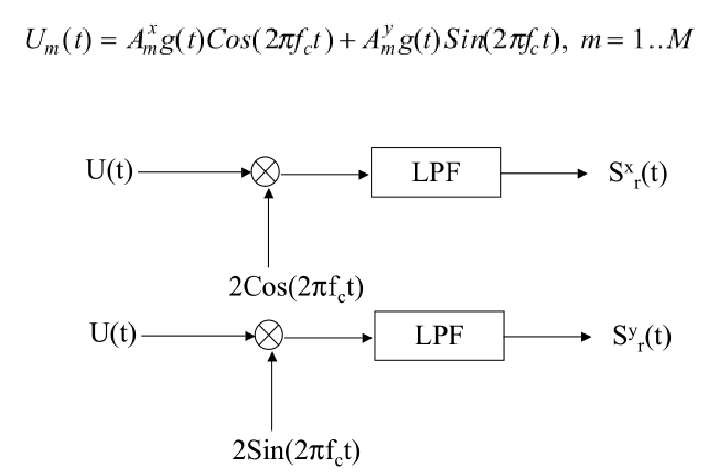
\includegraphics[width=0.5\textwidth]{img/wireless/MQAM demodulation.png}
        \caption{General schema of M-QAM demodulation}
        \label{fig:MQAM demodulation}
      \end{figure}
    \end{subsubsection}
    \begin{subsubsection}{Phase Shift Keying}
      \begin{boxH}
        \textbf{Phase Shift Keying}(PSK) is a PAM signal over the phase of a signal.\\
        In a PSK constellation, the amplitude of the signal is constant, meaning that
        all the signals have the same energy.
      \end{boxH}

      This means that the symbols are equally spaced across a circle of radius $\sqrt{E_S}$, where
      $E_S$ is the energy of the signal.\\
      Symbols are thus equally spaced to minimize the probability of error.\\

      \begin{figure}[h]
        \centering
        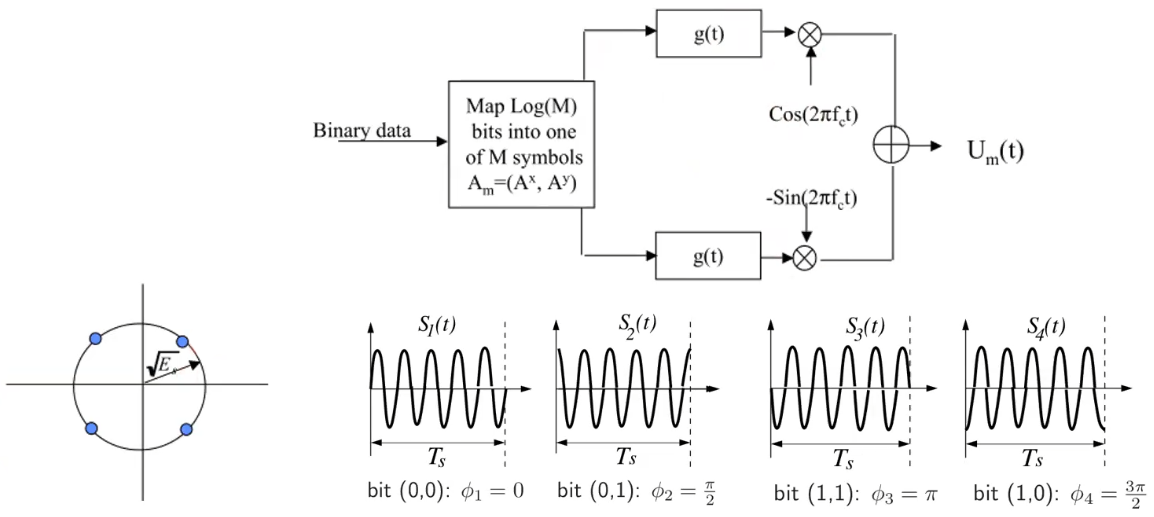
\includegraphics[width=0.7\textwidth]{img/wireless/MPSK modulation.png}
        \caption{General schema of M-PSK modulation}
        \label{fig:MPSK modulation}
      \end{figure}
      The modulation process is similar to the one of M-QAM. We can notice that, because all the 
      amplitude values are so similar, resulting the waveforms have the same energy.
    \end{subsubsection}

    \begin{subsubsection}{Power amplifiers}
      After modulation, the signal is usually amplified by a \textbf{power amplifier} to increase
      the power of the signal.\\
      \begin{figure}[h]
        \centering
        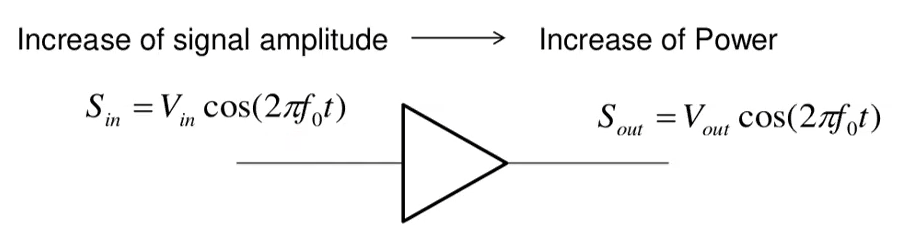
\includegraphics[width=0.5\textwidth]{img/wireless/power amplifier.png}
        \caption{General schema of a power amplifier}
        \label{fig:power amplifier}
      \end{figure}
      Because we cannot have infinite energy, we can only amplify the signal to a certain level, 
      which is called \textbf{saturation level}.\\
      This has some effect on the constellations of a signals:
      \begin{itemize}
        \item when working with \textbf{PSK} signals, the constellation in amplified uniformly
          even when working in saturation.
        \item when working with \textbf{QAM} signals, the constellation is scaled differently, 
          making the probability of error higher.
      \end{itemize}

      \begin{figure}[h]
        \centering
        \subfloat[PSK constellation after amplification]{
          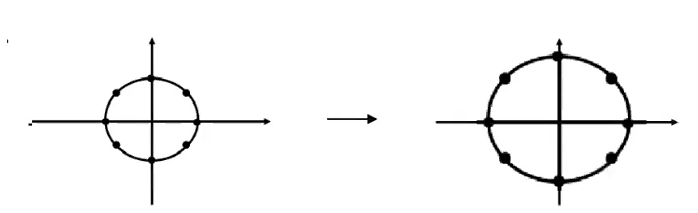
\includegraphics[width=0.4\textwidth]{img/wireless/PSK amplification.png}
          \label{fig:PSK amplification}
      }
        \hfill
        \subfloat[QAM constellation after amplification]{
          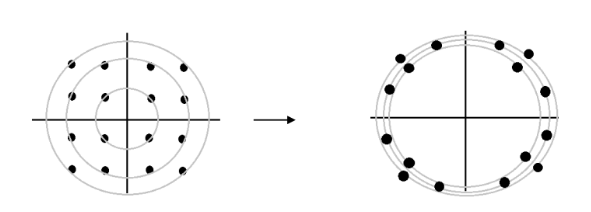
\includegraphics[width=0.4\textwidth]{img/wireless/QAM amplification.png}
          \label{fig:QAM amplification}
      }
        \caption{Effect of power amplification on a signal}
        \label{fig:constellation after amplification}
      \end{figure}
      When working under the saturation level, the power amplifier is linear, meaning that the
      output signal is proportional to the input signal, and no distortion occurs, but the 
      amplifier is underexploited.\\
      Thus, there is a trade-off between transmitted power and signal quality.\\
      
    \end{subsubsection}
  \end{subsection}

  \begin{subsection}{AWGN channel and equalization}
    Recall that to transmit information, we need to send a signal over a channel, in our case a 
    wireless one.\\
    We already briefly discussed the disturbance of a signals in subsection \ref{subsec:channel}, but the 
    main challenges can be summarized as:
    \begin{itemize}
      \item share the medium via \textbf{multiplexing}
      \item fight \textbf{noise} and \textbf{channel impairments}
    \end{itemize}
    The major sources of errors in the channel are essentualy two:
    \begin{itemize}
      \item \textbf{Termal noise}(AWGN), which is the result of the thermal agitation of the electrons
        in the receiver. It disturbs the signal in an additive fashion and occupies all the
        frequency band. Is also modelled by a Gaussian random process.
      \item \textbf{Inter-Symbol Interference}(ISI), which is the result of the signal being reflected
        by obstacles, and thus arriving at the receiver with a different phase and amplitude.
    \end{itemize}
    \begin{figure}[h]
      \centering
      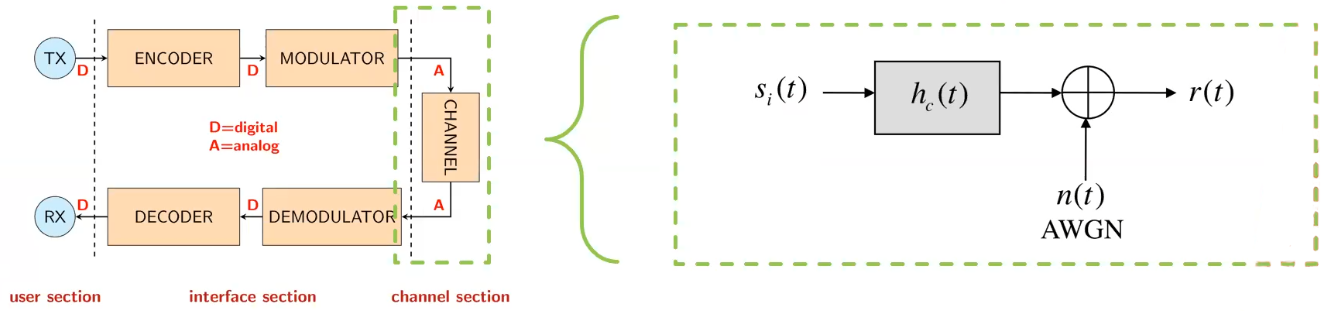
\includegraphics[width=0.8\textwidth]{img/wireless/channel effect.png}
      \caption{Effects of the channel on a signal, $h(t)$ is a filter that models the channel with it impusle response,
        and $n(t)$ is the noise}
      \label{fig:channel effects}
    \end{figure}
    We can say that the channel ruin the signal. This is evident when looking at the spectrum of the
    signal, which is spread by the channel, shown in figure \ref{fig:channel effect on the spectrum}.\\
    \begin{figure}[h]
      \
      \centering
      \subfloat[Effect of the noise on the signal]{
        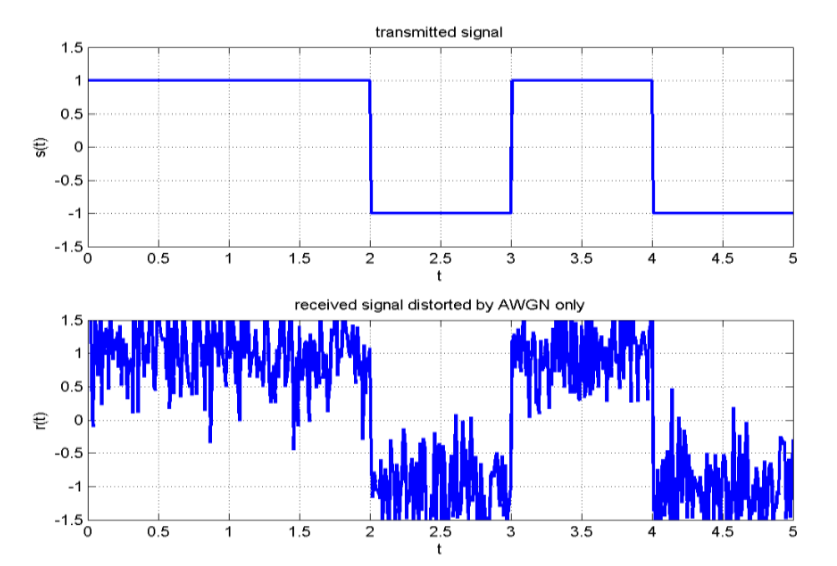
\includegraphics[width=0.4\textwidth]{img/wireless/signal AWGN effect.png}
        \label{fig:signal AWGN effect}
      }
      \hfill
      \subfloat[Signal spectrum distorted by inter-symbol interference, modelled by $h_c(t)$]{
        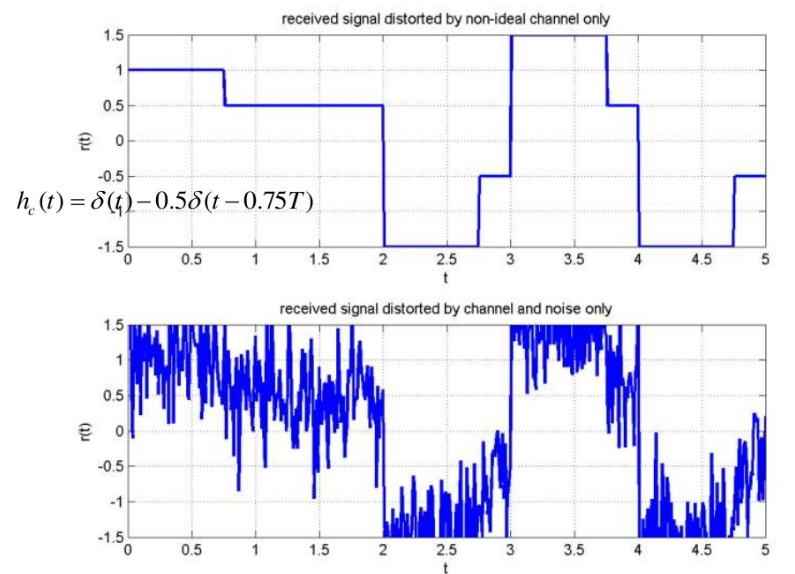
\includegraphics[width=0.4\textwidth]{img/wireless/signal filter effect.png}
        \label{fig:signal spectrum after channel}
      }
      \caption{Effect of the channel on the spectrum of a signal}
      \label{fig:channel effect on the spectrum}
    \end{figure}
    \begin{subsubsection}{Receiver Task}
      We want to design a receiver that can mitigate (or even revert) those two effects, to be 
      able to correctly understand the signal.\\
      To do so, we have to \textbf{demodulate} the signal and \textbf{equalize} it.\\
      This process can be carried out in 3 steps:
      \begin{enumerate}
        \item Improve the signal-to-noise ratio(SNR) using a \textbf{matched filter}
        \item Reduce Inter-Symbol Interference(ISI) using an \textbf{equalizer}
        \item Sample the recovered waveform and guess the transmitted symbol
      \end{enumerate}
      After those steps, we still have an imperfect signal wave, so we need to \textbf{detect} the
      transmitted symbol, thresholding the signals to remove outliers introduced in the channel 
      and decide with symbol was transmitted.\\
      \begin{figure}[h]
        \centering
        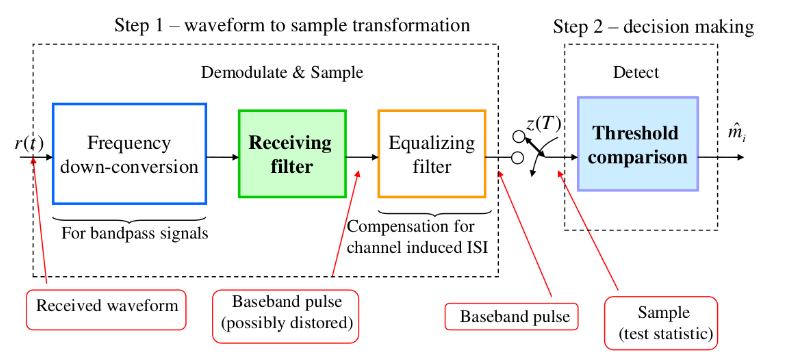
\includegraphics[width=0.8\textwidth]{img/wireless/receiver steps.png}
        \caption{General steps that a receiver has to carry out}
        \label{fig:receiver task}
      \end{figure}
    \end{subsubsection}

    \begin{subsubsection}{Maximize SNR}
      \begin{boxH}
        To maximize the signal-to-noise ratio, we can use a \textbf{matched filter} $h(t)=g(T-t)$
      \end{boxH}
      Turns out that the input response of the optimal filter is the time-reversed version of the
      pulse shape.\\
      The receiver must know the basic pulse shape to be able to use the matched filter.\\
      \begin{figure}[h]
        \centering
        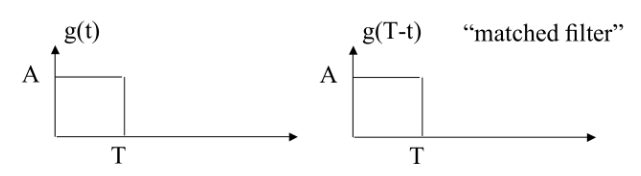
\includegraphics[width=0.6\textwidth]{img/wireless/matched filter.png}
        \caption{Effect of the matched filter on the signal. They are kind of the same because
        the function is symmetrical}
        \label{fig:matched filter}
      \end{figure}
    \end{subsubsection}

    \begin{subsubsection}{Minimize ISI}
      Inter-Symbol Interference is the result  of the filtering effect of the channel, and can be
      defined as 
      \begin{equation}
        H_c(f)=|H_c(f)|e^{j\phi_c(f)}
      \end{equation}
      where $|H_c(f)|$ is the amplitude response of the channel, which is non-constant meaning 
      that it distorts the amplitude of the signal, and $\phi_c(f)$ is the phase response of the
      channel, which is non-linear, meaning that it distorts the phase of the signal.\\

      To revert those effects, we can use an \textbf{equalizer} to compensate for the distortion
      of the channel, which ideally would be the inverse of the channel($H_e(f)=\frac{1}{H_c(f)}$).\\
      Applying it to the signal allows us to get an approximation of the original symbol that was
      transmitted $\hat{S_i}(t)$.\\

      To build the equalizer we still need to know the frequency response of the channel.
      To do that, we can try to estimate the channel based on known characteristics of the signal.
      Usually we don't know them, so we introduce \textbf{pilot symbols} in the signal, which are
      known signals to the receiver, and can be used to estimate the channel.
    \end{subsubsection}

    \begin{subsubsection}{Fading}
      Depending on the channel, its impulse response can vary very slowly or very quickly.\\
      When the impulse response varies slowly, we talk about \textbf{slow fading}, and when it
      varies quickly, we talk about \textbf{fast fading}.\\
      Depending on this, pilots symbols may need to be transmitted more or less frequently.\\
      \begin{figure}[h]
        \centering
        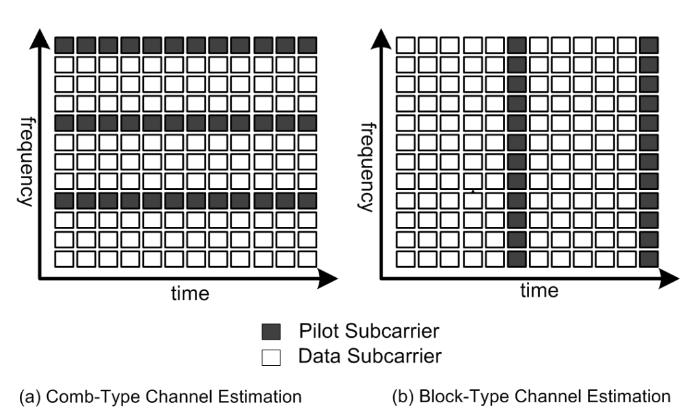
\includegraphics[width=0.6\textwidth]{img/wireless/pilot transmission scheme.png}
        \caption{Pilot transmission scheme}
        \label{fig:pilot transmission}
      \end{figure}
    \end{subsubsection}
  \end{subsection}
  \begin{subsection}{Received symbols and decision regions}
    After equalizing the signal, we would like to decide which symbol was transmitted.\\
    As previously stated, we get a set of possible symbols $S_m\in\{S_1,S_2,...,S_M\}$, and we
    want to decide which one was transmitted, adopting a statistical approach.\\
    \begin{subsubsection}{Symbol Detection}
      Mathematically speaking, we have an hypothesis testing problem, which wants to minimize the
      probability of decision error, meaning that we want to choose the symbol that maximizes the
      probability of the received signal given the transmitted symbol.\\
      
      This is known as the \textbf{Maximum a posteriori probability} (MAP) decision rule, which
      simplify that rule. In fact, turns out that maximizing the probability of the received signal
      given the transmitted symbol is equivalent to minimizing the distance between the received
      signal and the transmitted symbol, under certain conditions.\\
      This is also known as \textbf{Minimum distance decoding} $d_{rS_m}=(r-S_m)^2$, where $r$ is the
      received signal(actual value of the signal plus the noise).\\

      Take for example the case of a 2-PAM signal, shown in figure \ref{fig:signal detection example}.
      The noise alter the received signal, so we can define it as $r=S_m+n$, where $n$ is the noise.
      We also know that the noise is a Gaussian random process, so we can suppose that the noise is
      more likely will be zero, and its less likely will be far from it.\\
      This means that it is possible to assume that the received signal $r$ is more likely to be the
      symbol $S_m$ that is actually closer to it.\\
      So, in this case, we can define the decision region as the interval $[-\infty,0)$ and $(0,\infty]$,
      and the decision rule as
      \begin{equation}
        \hat{S_m}=\begin{cases}
          S_1 & \text{if } r<0\\
          S_2 & \text{if } r\geq 0
        \end{cases}
      \end{equation}
      This can also be generalized to the case of M-PAM signals, because the general idea is still valid.
      \begin{figure}[h]
        \centering
        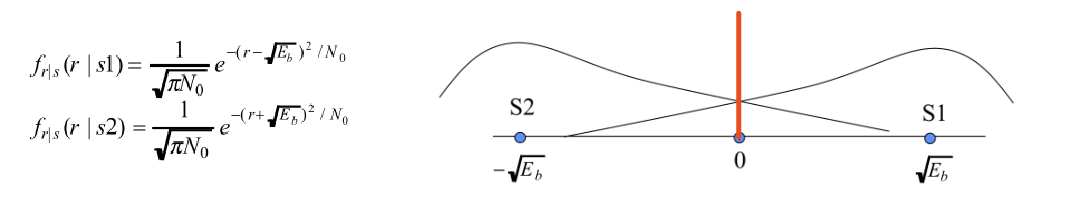
\includegraphics[width=0.8\textwidth]{img/wireless/signal detection example.png}
        \caption{Example of signal detection}
        \label{fig:signal detection example}
      \end{figure}
    \end{subsubsection}
    \begin{subsubsection}{Probability of error}
      The Minimum Distance Decoding rule adopts a statistical approach to decide which symbol was
      transmitted, so it is possible to make errors.\\
      In general, the probability of error $P_e$ between two symbols separated by a distance $d$ is
      \begin{equation}
        P_e=Q\left(\frac{d}{2\sigma}\right)
      \end{equation}
      where $Q$ is a complex function, and $N_0$ is the noise density.\\
      The probability of error can be minimized by increasing the distance between the symbols.

      Based on that we can compute the probability of error per bit, or Bit Error Rate(BER), for 
      each modulation scheme.\\
      Under certain condition, for example grey coding, the BER can be approximated as
      \begin{equation}
        BER=\frac{P_e}{\log_2(M)}
      \end{equation}
      \begin{figure}[h]
        \centering
        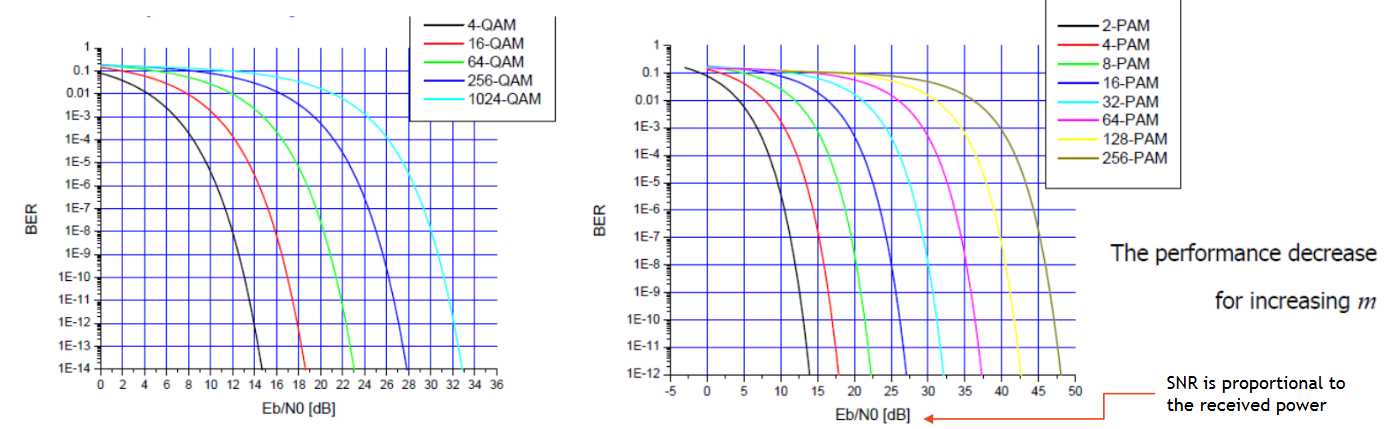
\includegraphics[width=\textwidth]{img/wireless/BER plots.png}
        \caption{Examples of BER plots for different modulation schemes. The BER is higher at the same 
        SNR for denser modulation schemes}
        \label{fig:BER plots}
      \end{figure}
    \end{subsubsection}
  \end{subsection}
  \begin{subsection}{Signal Attenuation and Link Budget}
    During the propagation of a signal, especially in wireless medium, it suffers from an 
    attenuation $L$, which is the loss of power of the signal.\\
    In general, it depends on many environmental factors, such as the distance between the
    transmitter and the receiver, the frequency of the signal, the presence of obstacles, and so on.\\

    The relationship between transmission and reception power is given by the $P_{R}=P_{T}/L$, where
    $P_{R}$ is the received power, $P_{T}$ is the transmitted power, and $L$ is the attenuation.\\
    Given this relationship, we can define the Signal-to-Noise Ratio(SNR) perceived by the receiver
    as
    \begin{equation}
      SNR=\frac{E_b}{N_0}
    \end{equation}
    where $E_b$ the ratio between the Received Power and the Bit Rate, and $N_0$ is the noise density.\\
    In general, to deal with this problem, we use antennas and amplifiers to increase the power of the
    signal and compensate for the attenuation. The shape of the antenna allows to modulate the
    rate of the signal: for example a wider antenna allows to spread the signal in a isotropic way
    and reach a wider area, while a more focused antenna allows to reach a more specific one.\\
    This is measure by the \textbf{beamwidth} of the antenna $\theta_B$, which is a measure of the 
    directivity of the antenna.\\

    \begin{boxH}
      The smaller the beamwidth, the more focused the antenna is, hence we yield a higher gain, but
      we also have a smaller area of coverage.\\
      The larger the beamwidth, the more isotropic the antenna is, hence we yield a lower gain, but
      we also have a larger area of coverage.\\
    \end{boxH}
    For example, a parabolic antenna has a very small beamwidth, so $\theta_B \approx 70\gamma/D$
    where $D$ is the diameter of the antenna.\\
    In general, the gain $G_T$ is proportional to the area of the antenna, so $G_T\propto 1/D^2$.
    Doubling the diameter of the antenna, we get a 4 times increase in the gain.\\

    \begin{figure}[H]
      \centering
      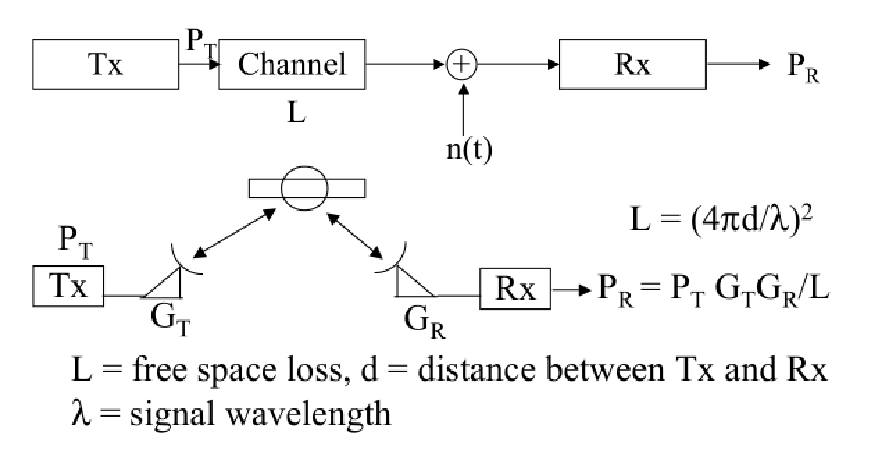
\includegraphics[width=0.6\textwidth]{img/wireless/signal attenuation.png}
      \caption{Example of signal attenuation over a wireless medium}
      \label{fig:antenna gain}
    \end{figure}
  \end{subsection}
  \begin{subsection}{Multiple Access Schemes}
    \begin{boxH}
      As previously discussed in section \ref{subsec:FDM}, we to trasmitt multiple signals over the same
      same shared medium, we have to use a method called \textbf{multiplexing}.
    \end{boxH}
    Multiplexing allows to divide the available bandwidth over multiple logical channels.\\
    The multiplexed signals are then transmitted over the same medium, and then demultiplexed at the
    receiver.\\

    Multiplexing on itself is not enough to allow multiple users to transmit over the same medium.
    We also need to use a method called \textbf{Multiple Access}, which allows multiple users to
    transmit over the same medium.\\
    \begin{boxH}
      \textbf{Multiplexing} deals with \textbf{combining signals}, while \textbf{multiple access} 
      deals with allowing \textbf{multiple users} to access and share a communication medium.
    \end{boxH}
    \begin{subsubsection}{Frequency Division Multiplexing/Multiple Access}
      As previously discussed, FDM allows to divide the available bandwidth over multiple logical
      channels.\\
      In the case of multiple access, we can use FDM to divide the available bandwidth over multiple
      users, and then modulating each user's signal over a different carrier frequency.\\
      This is done by assigning a different frequency band to each user, so that they can transmit
      over the same medium without interfering with each other.\\
      This is the case of \textbf{Frequency Division Multiple Access} (FDM/FDMA).\\
      With this schema, each user get access to the full bandwidth for the whole time, being able to
      completely avoid interference, but if the user is not transmitting, the channel is wasted.\\
      Furthermore, it is necessary to have a guard band between the channels to avoid interference.\\
      \textit{ All wireless systems use this scheme}.
      \begin{figure}[h]
        \centering
        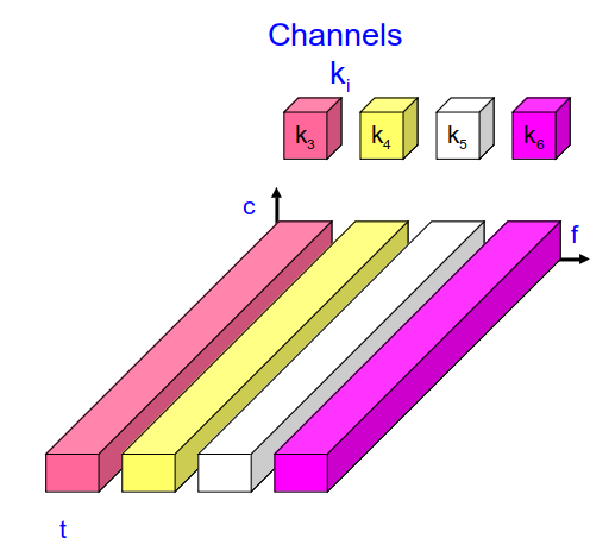
\includegraphics[width=0.4\textwidth]{img/wireless/FDMA.png}
        \caption{Example of FDMA}
        \label{fig:FDMA}
      \end{figure}
    \end{subsubsection}
    \begin{subsubsection}{Time Division Multiplexing/Multiple Access}
      TDM is a method that allows to divide the available bandwidth over multiple logical channels,
      by assigning a different time slot to each user.\\
      This slot is allocated to the user even if it has no data to transmitt. For this method to 
      work correctly some kind of synchronization is needed, but each communication channel has
      access to the full bandwidth, even if it is only for a fraction of the time.\\
      \begin{figure}[h]
        \centering
        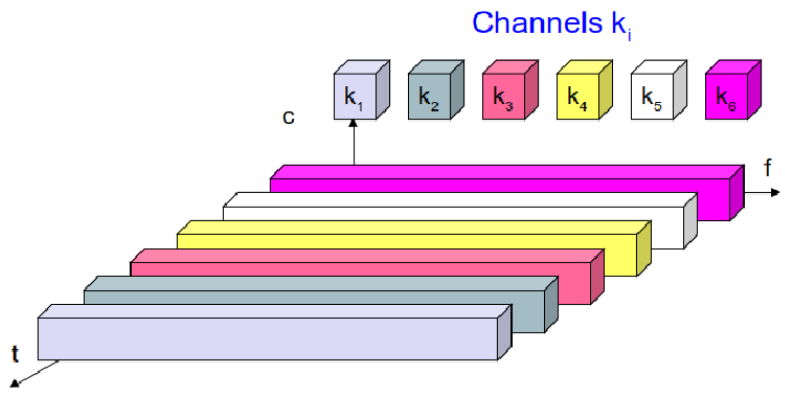
\includegraphics[width=0.4\textwidth]{img/wireless/TDMA.png}
        \caption{Example of TDMA}
        \label{fig:TDMA}
      \end{figure}
    In syncronous TDMA, many slots are wasted. There is a \textbf{statiscal version} of TDMA, called
    \textbf{STDM}, which reassigns the slots to the users that need them.\\
    This is done by scanning the input lines an collecting data until the frame is full, and then
    transmitting the frame.\\
    This method allows to avoid wasting slots, but it is more complex to implement, requiring 
    scheduling algorithms.\\
    \end{subsubsection}
    \begin{subsubsection}{Code Division Multiple Access}
      CDMA is a method that allows to divide the available bandwidth over multiple logical channels,
      by assigning a different code to each user.\\
      This method allows to exploit orthogonality between signals(allowing to separate them). Each
      channel has an unique code, while sharing the same spectrum(all of it) at the same time.\\
      Each channel is assigned a different code, and the receiver uses the unique binary code $c_i$
      of a sender to separate the signal from the others.\\

      For example a multiplexed signal
      \begin{equation*}
        s_{mux}(t)=s_1(t)c_1+s_2(t)c_2+s_3(t)c_3
      \end{equation*}
      is demultiplexed by the receiver using the code $c_1$ of the first sender
      \begin{equation*}
        \langle s_{mux}(t),c_1\rangle=s_1(t)
      \end{equation*}
      In this way, we are able to achieve a great bandwidth efficiency, with no need for coordination
      or synchronization while also getting a good degree of protection against interference.\\
      There are also some drawbacks: we have lower user data rates, and the system is more complex
      because the signals are more complex to regenerate.\\
      \begin{figure}[h]
        \centering
        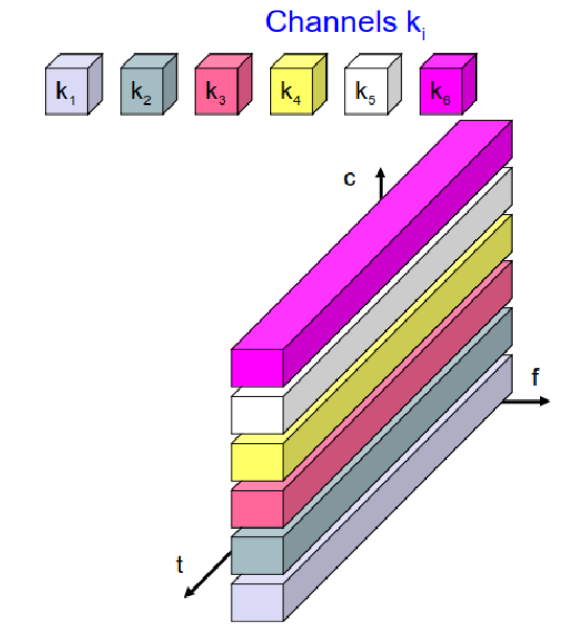
\includegraphics[width=0.4\textwidth]{img/wireless/CDMA.png}
        \caption{Example of CDMA}
        \label{fig:CDMA}
      \end{figure}
    \end{subsubsection}
    \begin{subsubsection}{TDM/A + FDM/A}
      It is also possible to combine the two methods.
      We can combine the time and frequency division multiplexing, allowing to divide the available
      bandwidth over multiple logical channels, by assigning a different time slot and frequency band
      to each user.\\
      With this solution, we are able to achieve a better degree of protection against tapping
      and frequency selective interference, at the cost of higher data rates(compared to CDMA).\\
      This method also requires a precise coordination between the users.\\
      \begin{figure}[h]
        \centering
        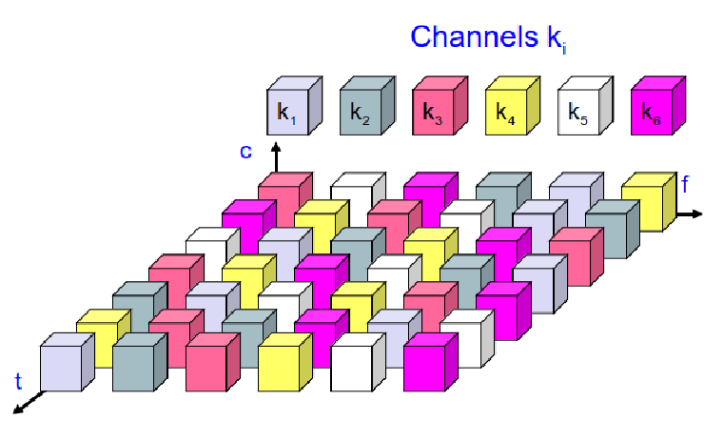
\includegraphics[width=0.4\textwidth]{img/wireless/TFDM.png}
        \caption{Example of TDMA/FDMA}
        \label{fig:TDMA/FDMA}
      \end{figure}
    \end{subsubsection}
  \end{subsection}

  \begin{section}{Source and channel coding}
    A brief overview: we have a source that generates a message, which is then encoded by the source
    encoder, to limit the amount of bits transmitted and the effects of noise.\\
    Those bits are then transformed into waveforms, which are altered by the channel, and then
    transformed back into bits by the channel decoder, after inverting the effects of the channel.\\

    Part of this operation are carried out in two steps:
    \begin{itemize}
      \item \textbf{Encoding}: which aims to produce a compressed representation $Y$ of the original
        message $X$. Usually encoding is simply a function $f$ that maps $X$ to $Y$.
      \item \textbf{Decoding}: which aims to recover the original message $X$ from the representation
        $Y$. Usually decoding is simply a function $f^{-1}$ that maps $Y$ to $X$.
    \end{itemize}
    \begin{figure}[h]
      \centering
      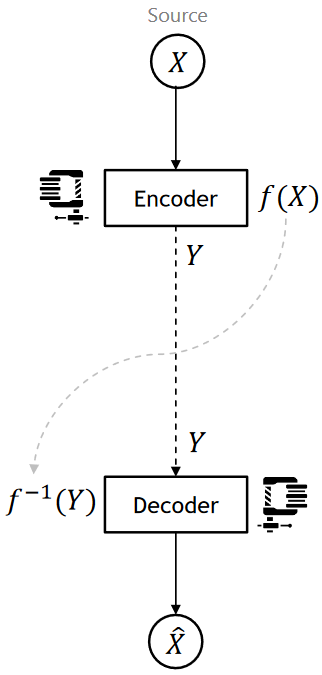
\includegraphics[width=0.2\textwidth]{img/wireless/encoding and decoding.png}
      \caption{General schema of encoding and decoding}
      \label{fig:encoding and decoding}
    \end{figure}

    \begin{subsection}{Source Coding}
      We would like to choose a encoding function $f$ that can be reverted while also \textbf{reducing
        redundancy} in the message.\\
        \begin{boxH}
          \textbf{Source coding}, also known as data compression, aims to represent information or
          data in a more compact form to reduce redundancy and save storage space or transmission 
          bandwidth.
        \end{boxH}
        This is possible because many real-world datasets exhibit patterns or repetitions that can 
        be efficiently encoded

        \begin{figure}[h]
          \centering
          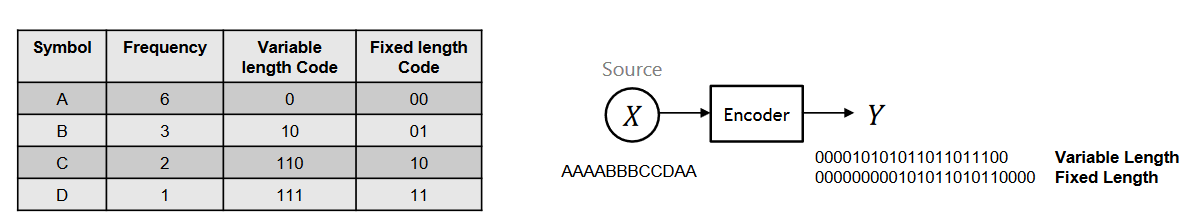
\includegraphics[width=\textwidth]{img/wireless/source coding.png}
          \caption{Example of source coding}
          \label{fig:source coding}
        \end{figure}

        Figure \ref{fig:source coding} shows an example of source coding. The example supposes that
        a sequence of letters is being transmitted. A possible uncompressed representation of the 
        letters would be assigning a two bit code to each letter(fixed length code).\\
        An alternative strategy exploits the fact that some letters are more frequent than others,
        assigning shorter codes to the most frequent letters(variable length code). With this
        solution, we are able to reduce the number of bits needed to transmit the message.\\
        \begin{subsubsection}{Compression Types}
          There are two main compression classes:
          \begin{itemize}
            \item \textbf{Lossless Compression}: the original data can be perfectly reconstructed
              from the compressed data($\hat{X}=X$). This is useful when the original data must be 
              preserved exactly, such as in text or executable files. Some examples of lossless
              compression includes ZIP, RAR, and PNG.
            \item \textbf{Lossy Compression}: the original data cannot be perfectly reconstructed
              from the compressed data($\hat{X}\approx X$). This is useful when the original data 
              can be approximated or when some loss of quality is acceptable, such as in images 
              or audio files.
          \end{itemize}
          As there are no officials compression formats, the specifications are defined by the
          fidelity requirements of the application. Generally, there is a trade-off between the
          compression efficiency and the computational complexity of the algorithm.
        \end{subsubsection}
    \end{subsection}

    \begin{subsection}{Error Detection and Correction}
      After compression, all the redundancy of the message has been possibly removed, and the bits
      that make up the message are the ones to be transmitted.\\
      Ideally, the message should be received unaltered, but we know that the channel can introduce
      errors in the message.\\
      Error detection techniques allow detecting such errors, while error correction enables 
      reconstruction of the original data. But those schemes add some redundancy to the message.\\
      For doing this, there are two main approaches:
      \begin{itemize}
        \item \textbf{Automatic Repeat request(ARQ)}: it implements acknowledgements and timeouts
          to ensure that the message is correctly received. 
        \item \textbf{Forward Error Correction(FEC)/Channel coding}: it adds redundancy to the 
          message to allow
          the receiver to correct errors without the need for retransmission.
      \end{itemize}
      \begin{subsubsection}{Channel Coding}
        Channel coding aims to detect and correct errors that may occur during transmission.\\
        It adds redundant bits to the original message, creating a coded message that contains 
        extra information for error detection and correction.\\
        The effectiveness of a channel code is often measured by its error correction capability,
        indicating the maximum number of errors that can be corrected within a codeword.\\

        There are two main types of channel coding:
        \begin{itemize}
          \item \textbf{Block Codes}: the message is divided into blocks of fixed length, and a 
            fixed number of redundant bits are added to each block. The receiver uses the redundant
            bits to detect and correct errors.
          \item \textbf{Convolutional Codes}: the message is encoded using a convolutional encoder,
            which adds redundant bits based on the current and previous bits of the message. The 
            receiver uses a Viterbi decoder to detect and correct errors.
        \end{itemize}
      \end{subsubsection}
      \begin{subsubsection}{Block Codes}
        A block code acts on block of $k$ bits of input data to produce $n$ bits of output data.
        This operation is carried out by the channel encoder.\\
        It simply adds $n-k$ bits of redundancy to the original message, which can be used by the
        receiver to detect and correct errors.\\

        \begin{figure}[h]
          \centering
          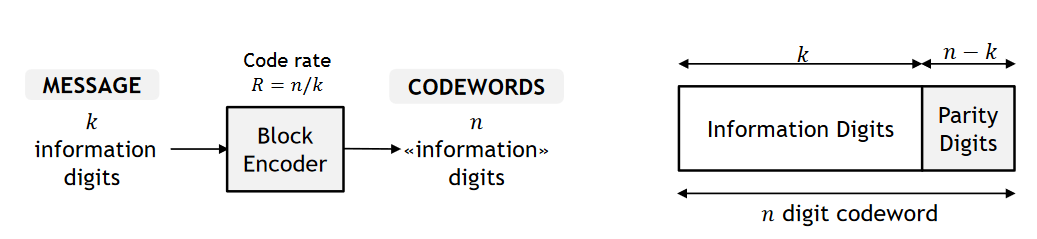
\includegraphics[width=\textwidth]{img/wireless/block codes.png}
          \caption{Example of block code}
          \label{fig:block code}
        \end{figure}
      \end{subsubsection}
    \end{subsection}
  \end{section}
  \begin{section}{Questions and answers}
    \begin{subsubsection}{In a digital communication system, what is the role of source encoding and
      decoding? What is its main goal? Describe the working principle(s)}
      In a digital communication system, the communication is, as the name suggests, digital. The
      thing is, the channel is only able to carry analog signals, meaning that we need an interface
      to convert the digital signal into a an analog one, and vice versa. The user portion of the
      interface section of a digital communication schema, at first apply source encoding, reducing
      the number of bits to be stransmitted, and channel encoding, which makes the sequence more
      robust, all this in a modulator, and the data is at last converted to analog by an encoder.
      The receiver gets the analog signals and sample it with a decoder, from which a demodulator is
      able to retreive the digital data, even perfectly if the sample frequence is high enough, by
      doing channel and source decoding, which corrects errors and recovers the original message.
    \end{subsubsection}

    \begin{subsubsection}{Describe how different signals can coexist over the same wireless medium.}
      Different signals can coexist over the same shared medium thanks to a method called
      multiplexing, which allows to divide the available bandwidth over multiple logical channels.
      There are different multiplexing schemes:
      \begin{itemize}
        \item Frequency division multiplexing: thanks to the modulation and demodulation of signals,
          we can transmitt different signals with overlapping bandwidth, by modulating each signal
          at a different frequency. This schema require a guard band between channels to avoid
          interference, and it is basically used by all wireless systems, because each channel has
          access to the full bandwidth for the whole time.
        \item Time division multiplexing: the bandwidth is divided between the logical channels 
          by assigning a time slot to each user, even if no data has to be transmitted.
        \item Code division multiplexing allows to divide the available bandwidth over multiple
          logical channels, by assigning a different code to each user, which is used to separate
          the signal from the others, which share the same spectrum at the same time, by exploiting
          the orthogonality between signals.
      \end{itemize}
    \end{subsubsection}

    \begin{subsubsection}{Describe the tradeoff between bandwidth efficiency and energy efficiency
      in digital modulations.}
      We know that to achieve a higher bandwidth efficiency, one has to use a lower bandwidth. 
      Symbols are distributed over the bandwidth, and the larger the energy, the larger
      the bandwidth, and thus the distance between symbols. With a smaller bandwidth, those are
      cramped in a smaller "space". But using a smaller bandwidth means that we are using a larger
      base pulse, which occupies less bandwidth but require more energy. This means that if we
      choose to occupy a smaller bandwidth, the transmitted sequence is more prone to errors,
      because symbols are closer to each other, and require less energy to be transmitted. on the
      other hand, if we add more space inbetween symbols, we will occupy a larger bandwidth, which
      requires less energy to be transmitted and is less prine to errors.
    \end{subsubsection}

  \end{section}
\end{section}

\chapter{Security at the physical layer}
As already mentioned in section \ref{sec:intro}, the wireless channel has no inherent security mechanisms. 
As a result, The wireless communication medium is open to \textbf{jamming} (or interference) and 
\textbf{eavesdropping} attacks from intruders.\\
Furthermore, the attacks can be classified into two categories: 
\begin{itemize}
    \item \textbf{Passive attacks}: the attacker only listens to the communication between the 
      two parties, without disrupting the network operation.
    \item \textbf{Active attacks}: the attacker can interfere in the communication between the 
      two parties.
\end{itemize}
\begin{figure}[H]
    \centering
    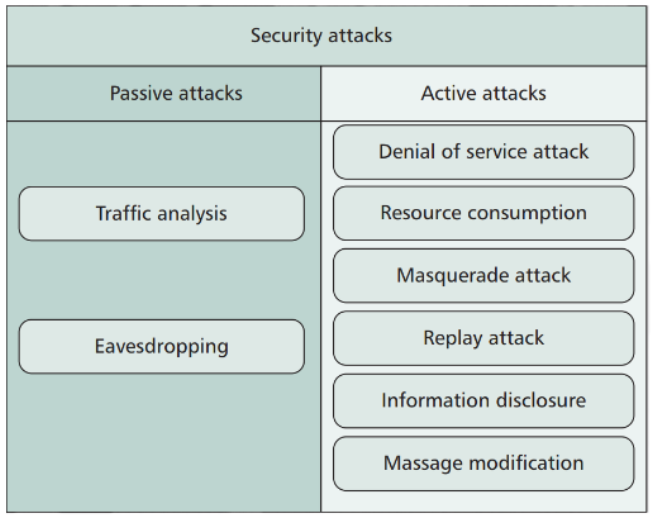
\includegraphics[width=0.5\textwidth]{img/wireless/attack classification.png}
    \caption{Active and passive attacks}
    \label{fig:active_passive_attacks}
\end{figure}
We are going to go through some of the most common attacks in wireless communication.
\begin{section}{Jamming}
   \begin{boxH}
     Jamming is a simple strategy to disrupt wireless communication by interfering with the
     communication channel.
    \end{boxH}
    It is usually carried out by broadcasting an interfering signal on a broad spectrum of frequencies
    to block the communication.\\
    A persistent and powerful adversary can always jam all data transmissions by transmitting 
    high-power white noise over the entire frequency spectrum.
    Jammer can be classified into two categories:
    \begin{itemize}
      \item \textbf{Active jamming}: the attacker continuously transmits a jamming signal to 
        interfere with the communication.
      \item \textbf{Reactive jamming}: the attacker only transmits a jamming signal when it
        detects a signal from the legitimate transmitter.
    \end{itemize}
    Although jamming is a difficult to address availability issue, it can be addressed via many
    physical layer security techniques.
    \end{section}
    \begin{section}{Eavesdropping}
      The wireless communication channel is a broadcast medium by nature. Because of this its 
      hard to eliminate unauthorized access to the wireless channel.\\
      To address those problesm, the most common way is to encrypt the data before transmitting it.\\
      Another widely used approach is to force the transmitter and receiver to adopt some 
      information hiding measures, by embedding private messages into a background signal or 
      noise process. In other words, we bury the information in the noise.\\
      Eavesdropping too can be addressed via physical layer security techniques.
\end{section}

\begin{section}{Physical Layer Security}
  In traditional systems, reliability is guaranteed by channel coding at the physical layer, while 
  security is ensured by encryption protocols at the upper layers, although in some cases we would 
  like to have security at the physical layer.\\
  This is possible because the physical layer has some unique properties that can be exploited to
  provide security, nominally the randomness of the wireless channel, which is an unpredictable
  and time-varying medium.\\

  \begin{boxH}
    \textbf{Physical layer security} aims at \textbf{exploiting the randomness} inherent in noisy channels to provide
    an additional level of protection at the physical layer.
  \end{boxH}
  
  \begin{figure}[h]
    \centering
    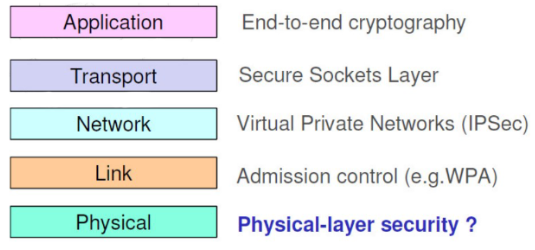
\includegraphics[width=0.5\textwidth]{img/wireless/layer security.png}
    \caption{Security measures at different layers}
    \label{fig:layer_security}
  \end{figure}
  A desirable proprety of the communication channel is \textbf{perfect secrecy}, which for a 
  wireless communication channel means that the channel is unknown to unauthorized users, or the 
  channel of the unauthorized users is more noisy than that of the authorized users.\\
  This means that we have a "better" channel than the eavesdropper, and we can obtain a that in 
  a different ways. For instance the sender and the receiver can cooperate, for example by choosing
  the same channel estimation method.\\

  In any case, security at physical layer is not intended to replace cryptographic security, but rather, it
  affords an additional protection layer. In fact, Physical Layer Security does not even allow 
  demodulation, which cryptographic security does.\\
  Nowadays, many results from information theory, signal processing, and cryptography
  suggest that there is much security to be gained by accounting for the imperfections of the
  physical layer when designing secure systems.

  Furthermore, physical layer security methods can be categorized into:
  \begin{itemize}
    \item \textbf{channel approaches}: such as fingerprinting, precoding and applying MIMO techniques.
    \item \textbf{code approaches}: adding cryptografy to error correction codes and applying spreading
      codes to the signal.
    \item \textbf{power approaches}: using direction antennas to make the communication less broad 
      or generating artificial noise to confuse the eavesdropper.
    \item \textbf{signal design approaches}: using artificial noise to degrade eavesdropper's 
      channel estimation
  \end{itemize}

  Each method addresses specific aspects of physical layer security, ranging from utilizing
  channel characteristics to employing artificial noise and directional antennas, and each one 
  is effective against different types of attacks.
  \begin{figure}[H]
    \centering
    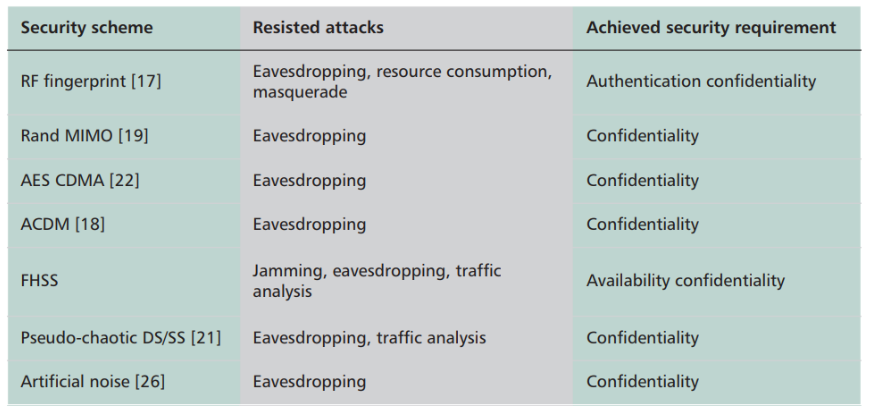
\includegraphics[width=0.8\textwidth]{img/wireless/physical layer security schema.png}
    \caption{Physical layer security methods}
    \label{fig:physical_layer_security_schema}
  \end{figure}

\end{section}


\chapter{GNSS and positioning}
  Global Navigation Satellite Systems (GNSS) are satellite-based systems that provide positioning, 
  navigation, and timing (PNT) services to users worldwide. The most well-known GNSS is the Global 
  Positioning System (GPS).\\
  The use of GPS and other GNSSs has become quite common in several civil application fields, (e.g.,
  transports and personal mobility, agriculture, ICT, ...), so Location Based Services (LBS) are
  becoming more and more important.\\

  In this chapter we will that GNSS users are particularly sensitive to some kinds of attacks, because
  those signals are very weak: for example Replaying broadcast GNSS signals with some delay 
  (meaconing), is enough to trick a user into a wrong position.\\
  \begin{section}{The positioning Problem}
    First of all, we need to define what is a position.\\
    \begin{boxH}
      A position is a set of coordinates, one for each dimension, associated with a reference 
      system.
    \end{boxH}
    \begin{figure}[h]
      \centering
      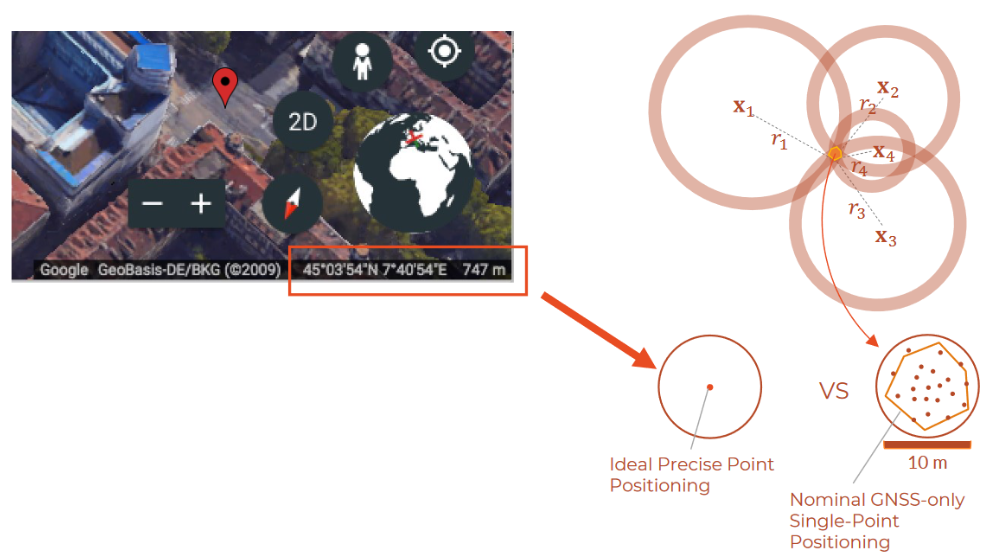
\includegraphics[width=0.8\textwidth]{img/wireless/GNSS position.png}
      \caption{Positioning in a 3D space}
      \label{fig:GNSS position}
    \end{figure}
    As shown in picture \ref{fig:GNSS position}, ideally we would like to have a system that can
    get a precise point positioning over a space, but in reality what we get is a cloud of points
    around the real position, from which the real position is estimated, withing a certain confidence
    interval.\\

    That being said, how is a position estimated?\\
    The information needed to estimate a position is provided by a set of sensors installed on 
    a terminal, such as a smartphone or a GPS receiver.\\
    Some of the most common sensors used are:
    \begin{itemize}
      \item \textbf{Satellite Navigation Chipset}, such as a GPS sensor, which tracks the signals
        from the satellites.
      \item \textbf{Inertial systems}, such as accelerometers and gyroscopes that measure the 
        acceleration and the angular velocity of the terminal.
      \item \textbf{Electronic Compasses}, which provide the orientation of the terminal.
      \item \textbf{Barometers}, which measure the atmospheric pressure.
      \item $\dots$
    \end{itemize}

    Because using all that sensors together to estimate a position is ideal but quite complex,
    a \textbf{data fusion algorithm} is used to combine the information from the sensors and estimate
    the position.\\
    \begin{figure}[h]
      \centering
      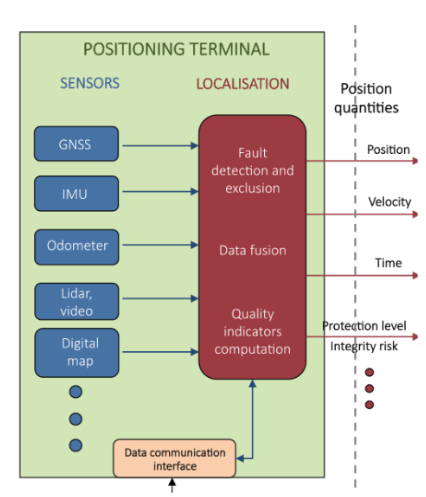
\includegraphics[width=0.3\textwidth]{img/wireless/data fusion algorithms.png}
      \caption{Representation of a data fusion algorithm}
      \label{fig:GNSS data fusion}
    \end{figure}
    In some cases using only the information provides is not enough to estimate a position, so
    some \textit{tricks} are used to improve the accuracy of the position estimation.\\
    For example google maps, when it gets an off road position, uses the information provided and
    maps the position to a point between some landmarks positioned on the road, as shown in picture
    \ref{fig:maps example}.\\

    \begin{figure}[h]
      \centering
      \includegraphics[width=0.6\textwidth]{img/wireless/maps example.png}
      \caption{Example of position estimation using landmarks}
      \label{fig:maps example}
    \end{figure}
  \end{section}

  \begin{section}{Satellite Navigation Systems and Segments}
    A little of history: the first satellite navigation system was put in space by the US Department
    of Defense in 1978. But it was only in the early 2000s that the system was opened to civil users.\\
    The european counterpart of the GPS is the Galileo system, which was put in space in 2017.\\
    \begin{figure}[h]
      \centering
      \includegraphics[width=0.9\textwidth]{img/wireless/GNSS history.png}
      \caption{History of GNSS systems}
      \label{fig:GNSS systems history}
    \end{figure}
    To provide a global coverage, a GNSS system is composed of a constellation of satellites, which
    are positioned in such a way that at least 4 satellites are visible from any point on the Earth.\\

    There are 4 main GNSS systems nowadays:
    \begin{itemize}
      \item \textbf{GPS} (USA)
      \item \textbf{Galileo} (Europe)
      \item \textbf{GLONASS} (Russia)
      \item \textbf{Beidou} (China)
    \end{itemize}
    which orbits at different altitudes and inclinations.\\
    Each of those systems  continuously transmit navigation signals in different frequencies in $L$ 
    band, as shown in picture \ref{fig:GNSS band}.\\

    \begin{figure}[h]
      \centering
      \includegraphics[width=0.8\textwidth]{img/wireless/GNSS band.png}
      \caption{Division of the $L$ band for GNSS systems}
      \label{fig:GNSS band}
    \end{figure}

    All those system are composed of 3 main segments:
    \begin{itemize}
      \item \textbf{Space Segment}, which is composed of the satellites, which continuously transmit
        the signals.
      \item \textbf{Control Segment}, which is composed of the ground stations that monitor the 
        satellites and send them the corrections.
      \item \textbf{User Segment}, which is composed of the users that receive the signals from the
        satellites and estimate their position. It performs 3 core functions:
        \subitem - Identification of the satellites in view
        \subitem - Measurement of the user-satellite distance
        \subitem - Run a PVT(Position, Velocity, Time) estimation algorithm
    \end{itemize}
    \begin{figure}[h]
      \centering
      \includegraphics[width=0.2\textwidth]{img/wireless/GNSS segments.png}
      \caption{Schema of the GNSS segments}
      \label{fig:GNSS segments}
    \end{figure}
    \begin{subsection}{GNSS signals}
      The GNSS satellites continuously transmit navigation signals in different frequencies in $L$ 
      band.\\
      Those signals are made up of different components, as shown in picture \ref{fig:GNSS signals}.\\
      The carrier modulate the data at the right frequency, the spreading code to perform multiple
      access, allowing to distinguish information from different satellites and demultiplexing the
      signals from the same satellite, , and the navigation data that contains the information 
      about the satellite position and the time.\\

      The navigation data allow the user to compute the travelling time from the satellite to the receiver,
      and the satellite position at any time.\\
      Using both the satellite position and the travelling time, the user can estimate its position
      , velocity and time(PVT).\\

      \begin{figure}[h]
        \centering
        \includegraphics[width=0.8\textwidth]{img/wireless/GNSS signal scheme.png}
        \caption{Scheme of the signals that make up the GNSS signal}
        \label{fig:GNSS signals}
      \end{figure}
    \end{subsection}

  \end{section}
  \begin{section}{Multilateration}
    Lets take a look at figure \ref{fig:GNSS multilateration problem}.\\
    We have a satellite that sends a signal $R_i$ to a user $x$, which would like to estimate 
    three coordinates $\langle x, y, z \rangle$.\\
    The signal contains the position of the satellite and the departure time of the message
    $T_{TX}$.\\
    The receiver measures the arrival time of the signal $T_{RX}$, and computes the distance
    between the receiver and the satellite $R_i$ as follows:
    \begin{equation}
      R_i = c\cdot \tau = c(T_{RX} - T_{TX})
      \label{eq:GNSS distance}
    \end{equation}
    where $c$ is the speed of light, which is the propagation speed of the signal, and $\tau$ is the
    \textit{time of flight} of the signal.\\
    In other words, the distance is the traveling time of the signal multiplied by propagation time
    in the free space.\\

    \begin{figure}[h]
      \centering
      \includegraphics[width=0.8\textwidth]{img/wireless/GNSS multilateration problem.png}
      \caption{Multilateration problem}
      \label{fig:GNSS multilateration problem}
    \end{figure}

    One measurement is not enough to estimate the position of the receiver, so at least 3 measurements
    are needed.\\
    \begin{boxH}
      We call this procedure \textbf{multilateration}, or the process of determining the position of an object
      by measuring the time of arrival of the signals from multiple sources.
    \end{boxH}

    But knowing the distance only tells us that the receiver is on a sphere centered on the satellite
    with radius $R_i$. It can be at any point on the sphere.\\
    If we have 2 satellites, we have 2 spheres, and the receiver is at the intersection of the two
    spheres.\\
    If we have 3 satellites, we have 3 spheres, and the receiver is at the intersection of the 3
    spheres.\\
    Unfortunately things are never that simple, but it gives the rough idea of how multilateration
    works.\\

    \begin{figure}[h]
      \centering
      \includegraphics[width=\textwidth]{img/wireless/multilateration comparison.png}
      \caption{Multilateration with 1, 2 and 3 satellites}
      \label{fig:Multilateration comparison}
    \end{figure}
  \end{section}
  \begin{section}{GNSS Functional basics}
    Lets add more detail to multilateration.\\
    If a satellite trasmit a pulse at time $t_0$, the receiver will receive it at time $t_0+\tau$,
    where $\tau$ is the time it takes for the signal to travel from the satellite to the receiver.\\
    We already saw in equation \ref{eq:GNSS distance} that the distance between the satellite and the
    receiver is equal to the time of flight of the signal multiplied by the speed of light.\\

    To get the distance, we only need to timestamp correctly the time of arrival of the signal.
    Yet, calculating the time of flight is not that simple, because the satellite and the receiver
    must be \textbf{synchronized} to allow the transmission time and the reception time to be on the 
    same time scale, and to be precise. Otherwise the distance estimation would be very off: 
    a signal that travels at the speed of light for 1 second travels 300000 km.\\
    In fact, the satellite host an \textbf{atomic clock}, which is a very precise clock that allows
    the satellite to timestamp the signal with a very high precision. They are also synchronized thanks
    to the control segment.\\
    The receiver also has a clock, but it is most likely not as precise as the atomic clock. 
    For this reason, the bias of the user torward the GNSS time scale $\delta t_u$ is unknown.\\
    The measured distance is then different from the geometric range and it is referred
    to as \textbf{pseudorange}, which is defined as:
    \begin{equation}
      \rho = c \cdot \tau + c \cdot \delta t_u
      \label{eq:GNSS pseudorange}
    \end{equation}

    There's also the bias of the satellite toward the scale $\delta t_u$. 
    This value is usually small and stable over time. The ground segment computes a bias $\delta t^S$
    that is uploaded to the satellite, and that the receiver can use to compute the right time of 
    flight.\\
    For those reason, we consider it to be zero, because it can be corrected.\\

    On the other hand, $\delta t_u$ cannot, the only thing we can do is keep it, so the position 
    is estimated by measuring the different pseudoranges from 4 different satellites, the minimum
    number of satellites in Line of Sight to estimate the position.\\
    This is because 3 satellites are needed to estimate the coordinates of a position, and the fourth
    satellite is needed to estimate the bias $\delta t_u$.\\
    If a larger number of satellites is in view a better estimation is possible.\\

    \begin{figure}[h]
      \centering
      \includegraphics[width=0.8\textwidth]{img/wireless/GNSS bias.png}
      \caption{Graphical representation of the bias $\delta t_u$ on the GNSS timescale}
      \label{fig:GNSS pseudorange}
    \end{figure}

    To sum it up, in GNSSs the user position is obtained through:
    \begin{itemize}
      \item \textbf{satellites} that broadcast that transmits timestamps.
      \item \textbf{Pseudoranges}, estimated trough one-way-arrival measurements
        receiver, plus the bias of the user toward the GNSS time scale.
      \item \textbf{Multilateration} based on the measurements
    \end{itemize}

    \begin{subsection}{The estimation problem}
      We have the measurements, but we need to estimate the position of the receiver.\\
      The relationship between the pseudoranges can be written as:
      \begin{equation}
        \begin{cases}
          \rho_1 = \sqrt{(x_1 - x_u)^2 + (y_1 - y_u)^2 + (z_1 - z_u)^2} + c\delta t_u\\
          \rho_2 = \sqrt{(x_2 - x_u)^2 + (y_2 - y_u)^2 + (z_2 - z_u)^2} + c\delta t_u\\
          \rho_3 = \sqrt{(x_3 - x_u)^2 + (y_3 - y_u)^2 + (z_3 - z_u)^2} + c\delta t_u\\
          \rho_4 = \sqrt{(x_4 - x_u)^2 + (y_4 - y_u)^2 + (z_4 - z_u)^2} + c\delta t_u\\
        \end{cases}
        \label{eq:GNSS pseudorange relationship}
      \end{equation}
      where $\langle x_i, y_i, z_i \rangle$ are the coordinates of the satellites(which are known),
      and $\langle x_u, y_u, z_u \rangle$ are the coordinates of the user(which are unknown as the bias).

      The goal is to invert the relationship and find the user coordinates and the bias given the
      pseudoranges.\\
      It is a non-linear estimation problem which is linearized through Taylor expansion 
      And solved through Least Mean Square Solutions or Bayesian Filters (e.g. Kalman).\\

      The generic pseudorange, which is a nonlinear relationship,
      \begin{equation*}
        \rho_i = \sqrt{(x_i - x_u)^2 + (y_i - y_u)^2 + (z_i - z_u)^2} + c\delta t_u
      \end{equation*}
      can be approximated through the Taylor expansion around a known location used as a linearization point
      (a point that is close to the real solution) $\langle \hat{x}_u, \hat{y}_u, \hat{z}_u, \hat{\delta t}_u \rangle$:
      \begin{equation*}
        \hat{\rho}_i = \sqrt{(x_i - \hat{x}_u)^2 + (y_i - \hat{y}_u)^2 + (z_i - \hat{z}_u)^2} + c\hat{\delta t}_u
        \label{eq:GNSS linearization}
      \end{equation*}
      To put it into a graphical prospective, take a look at figure \ref{fig:GNSS linearization}.\\
      If we choose a linearization point, we need to know the difference $\Delta x_u$ between the real
      position and the linearization point. If we can estimate it, which is easier because it is a 
      linear problem, we can estimate the user position.\\


      \begin{figure}[h]
        \centering
        \includegraphics[width=0.5\textwidth]{img/wireless/linearization scenario.png}
        \caption{Graphical representation of the linearization of the pseudorange in one dimension}
        \label{fig:GNSS linearization}
      \end{figure}
      We can expand this concept to the general formula \ref{eq:GNSS linearization} as the difference 
      between the real position and the linearization point:
      \begin{equation}
        \begin{cases}
          \Delta x_u = x_u - \hat{x}_u\\
          \Delta y_u = y_u - \hat{y}_u\\
          \Delta z_u = z_u - \hat{z}_u\\
          \Delta \delta t_u = \delta t_u - \hat{\delta t}_u\\
        \end{cases}
        \label{eq:GNSS linearization difference}
      \end{equation}
      The linearized pseudorange can be written as:
      \begin{equation}
        \delta \rho_j = \hat{\rho}_j - \rho_j = a_{xj}\Delta x_u + a_{yj}\Delta y_u + a_{zj}\Delta z_u + a_{tj}\Delta \delta t_u
        \label{eq:GNSS linearized pseudorange}
      \end{equation}
      The coefficients $a_{ij}$ are the partial derivatives of the pseudorange with respect to the
      user position and the bias, obtained through the Taylor expansion.\\
      They can be written as:
      \begin{equation}
        \begin{cases}
          a_{xj} = \dfrac{x_j - \hat{x}_u}{\hat{\rho}_j}\\
          a_{yj} = \dfrac{y_j - \hat{y}_u}{\hat{\rho}_j}\\
          a_{zj} = \dfrac{z_j - \hat{z}_u}{\hat{\rho}_j}\\
          a_{tj} = \dfrac{c}{\hat{\rho}_j}
        \end{cases}
        \label{eq:GNSS linearized coefficients}
      \end{equation}
      where 
      \begin{equation*}
        \hat{\rho}_j = \sqrt{(x_j - \hat{x}_u)^2 + (y_j - \hat{y}_u)^2 + (z_j - \hat{z}_u)^2} + c\hat{\delta t}_u
      \end{equation*}
      that being the geometrical distance between the linearization point and the satellite.\\
      This allows us to write our relationship as:
      \begin{equation}
        \begin{cases}
          \delta \rho_1 = a_{x1}\Delta x_u + a_{y1}\Delta y_u + a_{z1}\Delta z_u + a_{t1}\Delta \delta t_u\\
          \delta \rho_2 = a_{x2}\Delta x_u + a_{y2}\Delta y_u + a_{z2}\Delta z_u + a_{t2}\Delta \delta t_u\\
          \delta \rho_3 = a_{x3}\Delta x_u + a_{y3}\Delta y_u + a_{z3}\Delta z_u + a_{t3}\Delta \delta t_u\\
          \delta \rho_4 = a_{x4}\Delta x_u + a_{y4}\Delta y_u + a_{z4}\Delta z_u + a_{t4}\Delta \delta t_u\\
        \end{cases}
        \end{equation}
        that can be also rewrited in a matrix form as:
        \begin{equation}
        \begin{bmatrix}
          \delta \rho_1\\
          \delta \rho_2\\
          \delta \rho_3\\
          \delta \rho_4\\
        \end{bmatrix}
        =
        \begin{bmatrix}
          a_{x1} & a_{y1} & a_{z1} & a_{t1}\\
          a_{x2} & a_{y2} & a_{z2} & a_{t2}\\
          a_{x3} & a_{y3} & a_{z3} & a_{t3}\\
          a_{x4} & a_{y4} & a_{z4} & a_{t4}\\
        \end{bmatrix}
        \begin{bmatrix}
          \Delta x_u\\
          \Delta y_u\\
          \Delta z_u\\
          \Delta \delta t_u\\
        \end{bmatrix}
        \label{eq:GNSS linearized matrix}
      \end{equation}
      where $a_{tj}$ can be approximated as $1$ because the bias is usually small.\\
      This matrix representation is easier to invert, in fact 
      \begin{equation*}
        \delta x= H^{-1}\delta \rho
      \end{equation*}
      which is our solution: the user position.\\
      \begin{subsubsection}{The Least Squares Solution}
        The method above can only be used if the number of satellites is small(4 or less), because 
        otherwise the matrix $H$ would be non-square and non-invertible.\\
        If the number of satellites is larger, it is possible to use the Least Squares Solution.\\
        The solution would be 
        \begin{equation}
          \Delta x = (H^TH)^{-1}H^T\delta \rho
          \label{eq:GNSS least squares}
        \end{equation}
        where $H^T$ is the transpose of the matrix $H$.\\
      \end{subsubsection}
      \end{subsection}

    \begin{section}{Positioning Errors}
      We know that that channel is unpredictable, so the pseudorange is most likely affected by errors,
      due to things such as noise and propagation.\\
      We can redifine our pseudorange model as:
      \begin{equation}
        \rho_i = \sqrt{(x_i - x_u)^2 + (y_i - y_u)^2 + (z_i - z_u)^2} + b_{ut} + \epsilon
        \label{eq:GNSS pseudorange error}
      \end{equation}
      where $b_{ut}$ is the bias of the user toward the GNSS time scale, and $\epsilon$ is the error.\\

      We also need to modify the solution accordingly:
      \begin{equation}
        \Delta x = [(H^TH)^{-1}H^T]\delta \rho
        \label{eq:GNSS least squares error}
      \end{equation}
      where $\delta \rho$ is the error in the pseudoranges.\\
      Basically, we have a portion of the formula that depends on the geometry of the satellites(
      $(H^TH)^{-1}H^T$) and a portion that depends on the errors in the pseudoranges which is
      upredictable.\\
      As it is possible to observe, the position of the satellite influence the error in the pseudorange,
      fore example amplifying it.\\
      
      The causes of the errors in the pseudorange are shown in figure \ref{fig:GNSS errors}.\\
      The relativistic effect on the clock, the fact that even if the clocks are synchronized, they
      move at different speeds, can be corrected because it is predictable.\\
      The atmoshpere too influences the signal, but it can be corrected because it is predictable.\\
      Some of them cannot be corrected, such as the multipath effect, the fact that the signal can
      bounce off buildings and arrive at the receiver later than expected.\\

      \begin{figure}[h]
        \centering
        \includegraphics[width=0.8\textwidth]{img/wireless/GNSS errors.png}
        \caption{Causes of the errors in the pseudorange}
        \label{fig:GNSS errors}
      \end{figure}

      \begin{subsection}{User Equivalent Range Error}
        The summary of the total error budget affecting a pseudorange from the user's point of view 
        is called the \textbf{user equivalent range error} (UERE).\\
        Thus, we can model the pseudorange error as a random variable with a mean of $0$ and a standard
        deviation of $\sigma_{\text{UERE}}$.\\
        After correcting known sistematic errors, the unknown ones can be modelled as a Gaussian 
        distribution, with a mean of $0$ and a variance $\sigma_{\text{UERE}}^2$, obtained as the sum
        of other residual contributions:
        \begin{equation}
          \sigma_{\text{UERE}} = \sqrt{\sum_{j} \sigma^2_j [m]}
        \label{eq:GNSS UERE}
      \end{equation}
      \end{subsection}

      \begin{subsection}{The Geometrical Factor}
        Errors makes the solution more uncertain, but its not the only factor that influences the
        accuracy of the solution.\\
        The geometrical distribution of satellites affects the precision of estimated position too

        \begin{figure}[h]
          \centering
          \includegraphics[width=0.7\textwidth]{img/wireless/satellite distibution.png}
          \caption{Distrubution of the satellites ideally and in reality}
          \label{fig:GNSS geometry}
        \end{figure}

        It can be proved that, under some conditions, this geometrical effect on the positioning 
        error can be measured.
        the standard deviation of the positioning error can be obtained as:
        \begin{equation}
          \sigma_{x} = \sqrt{\sigma^2_{x_u} + \sigma^2_{y_u} + \sigma^2_{z_u} + \sigma^2_{b_{ut}}}
          =\text{GDOP} \cdot \sigma_{\text{UERE}}
          \label{eq:GNSS PDOP}
        \end{equation}
        where GDOP is the \textbf{Geometric Dilution of Precision}:
        \begin{equation}
          \text{GDOP} = \sqrt{tr\{[H^TH]^{-1}\}}
          \label{eq:GNSS GDOP}
        \end{equation}
        and $\sigma_{\text{UERE}}$ is the standard deviation of the pseudorange error.\\
      \end{subsection}
    \end{section}

    \end{section}

    \begin{section}{GNSS threats}
      GNSS is not that robust by itself, in fact the main source of signal degradation are:
      \begin{itemize}
        \item \textbf{evil waveforms}
        \item \textbf{multipath}
        \item \textbf{radio frequency interference}
        \item \textbf{spoofing}
      \end{itemize}
      The robustness of GNSS signals derives from the \textbf{spread spectrum} nature of the 
      transmitted signal (Direct Sequence Spread Spectrum), exploited also for CDMA purposes.\\
      Despite the spread signal structure, navigation receivers are vulnerable to (strong) 
      interfering signals, that might prevent the correct signal processing.\\

      In fact, the typical signal to noise ration of a GNSS signal is around $-30dB$, which 
      means that on normal conditions the signal is buried in the noise.\\
      Fortunately, spread spectrum is robust to the presence of interfering signals, but we still
      have to revert the spreading to recover the original signal.\\
      The product with the PRN code spreads the power over a larger bandwidth, making the bandwidth
      of a signal $B_x \simeq 50 - 250\text{Hz}$ much larger($B_{SS} \simeq 2-8\text{MHz}$).\\
      If an interference signal of bandwidth $B_i$ affects the signal, only a portion of the power 
      will be actually received as “additional noise”, because the rest of the power will be
      spread over the whole bandwidth.\\

      For this reason, the despreading operation made at the receiver spreads the power of the 
      interfering signal over a wide bandwidth($B_{SS}$), making the interference power density
      much lower than the signal power density.\\

      \begin{figure}[h]
        \centering
        \includegraphics[width=0.9\textwidth]{img/wireless/signal despreading.png}
        \caption{Effect of despreading over a signal bandwidth}
        \label{fig:GNSS despreading}
      \end{figure}
      \begin{subsection}{Interference classification}
        Because of the bandwidth size, we are actually able to classify interference, according to 
        the spectral and time features with relation to the GNSS signal:
        \begin{itemize}
          \item \textbf{Narrowband Interference}: $B_i \ll B_{SS}$
          \item \textbf{Wideband Interference}: $B_i \simeq B_{SS}$
          \item \textbf{Continuous Wave Interference}: the interference is continuous in time
            over a single frequency band, $B_i \to 0$
          \item \textbf{Pulse Interference}: the interference is pulsed in time
        \end{itemize}

        We can also distinguish between \textbf{Out-of-band interference} and \textbf{In-band
        interference}.\\
        The first one is interference that is outside the GNSS band, while the second one is
        interference that is inside the GNSS band. This means that OOB interference should not 
        affect the GNSS signal, while IB interference can, buth both of them can be problematic.\\

        \begin{figure}[h]
          \centering
          \includegraphics[width=0.7\textwidth]{img/wireless/in and out of band interference.png}
          \caption{Classification of interference}
          \label{fig:GNSS interference classification}
        \end{figure}

        A further distinction can be made between \textbf{Intentional Interference} and
        \textbf{Unintentional Interference}.\\
        The first one is interference that is intentionally generated to disrupt the GNSS signal,
        while the second one is interference that is generated by other devices, but that can still
        disrupt the GNSS signal, and is generally generated by OOB interference.\\
      \end{subsection}

      \begin{subsection}{Jamming}
        \begin{boxH}
          A \textbf{jammer} is a \textbf{device} that generates \textbf{interference} to disrupt the GNSS signal.\\
          Jamming objective is the denial of navigation service by masking the GNSS signal with
          noise.
        \end{boxH}

        Normally, signal radiation in the GNSSs bands is regulated by the ITU, and not legal.\\
        Those devices can be a severe threat for  liability-critical mass-market applications, 
        such as GNSS-based road tolling or fleet management.\\
        In general, Mass-market jammers usually aim at disturbing a wide band by 
        frequency-modulating a pure tone.\\

        Lets now try to understand the effect of jamming on the GNSS signal.\\
        In general, interference affect the receiver at different levels: at first we can observe 
        a spike in the noise level after the signal has been received, or we can observe a
        degradation of the signal quality.\\
        This means that we are able to understand if a signal is being jammed before the pseudorange
        is computed.\\

        The net effect is an error on the measured pseudorange $\rho$, and the effect depends on
        \begin{itemize}
          \item the receiver architecture(front-end filters, quantization bits, etc.)
          \item the structure of the GNSS signal(modulation, spreading, etc.)
        \end{itemize}
        Therefore detection and mitigation of interference can act at different stages of the 
        receiver itself:
        \begin{itemize}
          \item antenna shaping
          \item front-end filtering
          \item time domain blanking
          \item other transformed domains
        \end{itemize}

        \begin{figure}[h]
          \centering
          \includegraphics[width=0.7\textwidth]{img/wireless/jamming delay effect.png}
          \caption{Effect of jamming on the delay of a GNSS signal. The delay is increased by the
            jamming signal.}
          \label{fig:GNSS jamming effect}
        \end{figure}
        \begin{subsubsection}{Signal-to-Noise Ratio Monitoring}
          Aside from the spectrum, one other thing that can be monitored to detect jamming is the
          Signal-to-Noise Ratio(SNR).\\
          Strictly speaking, the interference is not noise, but from the user point of view it is
          indistinguishable from it. The net effect is that the SNR is affected by interference,
          contributing to the \textbf{noise variance}.\\

          Observing the SNR in some scenarios may allow to define a \textbf{statistical threshold}: 
          if the SNR is below a certain value, the signal may be jammed.\\

          Generally speaking, The only available output common to any GNSS receiver is the 
          carrier-to-noise-density ratio (C/N0) parameter, which is the ratio of the carrier power
          to the noise power spectral density, an estimated value closely related to SNR.\\
          The C/N0 is a good indicator of the signal quality, and it is used to detect jamming: in
          case of jamming, the C/N0 will decrease.\\
          \begin{figure}[h]
            \centering
            \includegraphics[width=0.3\textwidth]{img/wireless/c over n0.png}
            \caption{Example of a C/N0 measurements of a signal while being jammed.}
            \label{fig:GNSS CN0 monitoring}
          \end{figure}

        \end{subsubsection}
        \begin{subsubsection}{Spectral analysis}
          One of the most effective ways of detecting jamming is to perform a spectral analysis of the
          received signal.\\

          Figure \ref{fig:GNSS spectral analysis} shows the effect of interference on the spectrum
          of a GNSS signal.\\
          On the left is shown the effect of normal noise over the spectrum of the signal, while on
          the right is shown the effect of jamming.\\
          Is is evident when it is happening: you can clearly see it in the spectrum.\\

          \begin{figure}[h]
            \centering
            \includegraphics[width=0.7\textwidth]{img/wireless/spectrum effect.png}
            \caption{Effect of interference on the spectrum of a GNSS signal}
            \label{fig:GNSS spectral analysis}
          \end{figure}
        \end{subsubsection}
        \begin{subsubsection}{Automatic Gain Control Behavior}
          Another important detection strategy is to monitor the behavior of the Automatic Gain Control
          (AGC) of the receiver.\\

          The AGC is a system that automatically controls the gain of the receiver, in order to
          maintain the signal at a constant level, the optimal input range of the ADC(quantizer).\\
          \begin{figure}[h]
            \centering
            \includegraphics[width=0.4\textwidth]{img/wireless/AGC.png}
            \caption{Graphical representation of the AGC}
            \label{fig:AGC}
          \end{figure}
        It can be used to detect jamming, because the AGC will try to increase the increase the gain
        to maintain the signal at a constant level, but if the signal is jammed, the AGC will 
        decrease the gain because the signal is stronger.\\

        Because GNSS signals are weak, the AGC is usually set to a high gain, so if the AGC is
        decreasing the gain, it is a sign that the signal is being jammed.\\
        This is evident when looking at figure \ref{fig:AGC jamming}, which shows the gain level
        of the AGC over the time.\\
        n absence of interference the gain introduced by the AGC is constant over the time, or slowly
        changing, but in a hostile environment the average gain level is lower and the AGC
        gain is not constant.
        \begin{figure}[h]
          \centering
          \includegraphics[width=0.6\textwidth]{img/wireless/AGC jamming.png}
          \caption{Effect of jamming on the AGC}
          \label{fig:AGC jamming}
        \end{figure}
        The AGC also have some kind of effect over the spectrum of the signal, decreasing the magnitude 
        of the spectrum over the intermediate frequencies(IF), and which is variable over time.\\
        

        \end{subsubsection}
        \begin{subsubsection}{Goodness-of-Fit Test}
          For interference detection purposes, the IF samples at the output of the ADC can be used 
          to build the test statistic and make the decision.\\
          The test performs the comparison of two Probability Density Functions (histograms),
          allowing the decision between two hypotheses. The PDFs are approximated by the histograms of
          the samples.
          
          If the thermal noise is dominating the samples distribution (nominal behavior), the 
          histogram should exhibit a \textbf{Gaussian shape}.
          On the other hand, In the case of the presence of an interference source, the histogram 
          will modify its regular shape, enabling the test to detect such a distortion.\\
          The bins needed for evaluating the discrete version of the PDF are directly arranged by 
          the signal quantization levels.

          \begin{boxH}
            In the \textbf{interference free} case the noise dominates the GNSS signal and the statistic of 
            samples is expected to be \textbf{Gaussian}.
          \end{boxH}

          \begin{figure}[h]
            \centering
            \includegraphics[width=0.8\textwidth]{img/wireless/good to fit test.png}
            \caption{Goodness-of-Fit test}
            \label{fig:GNSS goodness of fit}
          \end{figure}
        \end{subsubsection}

        \begin{subsubsection}{Machine learning on interference monitoring}
          The interference detection is a typical classification task in supervised machine 
          learning. The reason is to build a prediction model tp bredict the outcome based on 
          a set of input variables.\\
          The model is trained based on the detected jamming signals reported in literature.\\
          This is done by extracting features from the signal, both in the time domain and in the
          frequency domain, and then using these features to train a machine learning model.\\

          \begin{figure}[h]
            \centering
            \includegraphics[width=0.8\textwidth]{img/wireless/training features.png}
            \caption{Features extraction for machine learning}
            \label{fig:GNSS machine learning}
          \end{figure}
        \end{subsubsection}

      \begin{subsubsection}{Mitigation with domain techniques}
        For mitigation, we want to identify our interference precisely, in the time domain
        or frequency domain, depending on the nature of the interference.\\
        A continuous wave interference can be easily detected in the frequency domain, unlike in the 
        time domain, because the interference is occupying a single frequency band.\\

        To do so we can use a \textbf{notch filter}, which is a filter that removes a certain
        frequency band from the signal.\\

        \begin{figure}[h]
          \centering
          \includegraphics[width=0.9\textwidth]{img/wireless/notch filter.png}
          \caption{Notch filter}
          \label{fig:GNSS notch filter}
        \end{figure}

        In the time domain, we can understand when the interference is happening, and we can
        remove the interference by blanking the signal via \textbf{digital pulse blanking}, which 
        blanks both the signal and the interference.\\

        \begin{figure}[h]
          \centering
          \includegraphics[width=0.7\textwidth]{img/wireless/digital pulse blanking.png}
          \caption{Pulse blanking}
          \label{fig:GNSS pulse blanking}
        \end{figure}
      \end{subsubsection}
    \end{subsection}

    \begin{subsection}{Spoofing}
      \begin{boxH}
         Spoofing refers to the transmission of fraudulent GNSS-like signals, that force the
         victim receiver to compute erroneous positions
      \end{boxH}
      It is another big threat for GNSS. This kind of attack has been present in the military 
      field, but with the extensive use of GNSS it may threat several applications.\\

      Furthermore, while jamming is easily detectable, spoofing is not, because the signal is
      not masked by noise, but it is a signal that is very similar to the GNSS signal.\\
      For this reason, attacks can be very effective depending on the quality of the generated 
      signal.\\

      Denial of service is not the only possible attack, but by spoofing the signal, the attacker
      can also manipulate the position of the receiver, for example to fraud a tolling system.\\
      Such menaces also apply to safety-critical applications (e.g. Advanced Driver Assistance 
      Systems(ADAS), eCall).\\

      An ideal spoofer must be as much as possible consistent with the real signals, in fact it must
      \begin{itemize}
        \item Match the signals from expected visible satellite
        \item be synchronized with the GNSS time scale
        \item match the directing of arrival
        \item be realistic terms of power an Doppler effect(velocity)
      \end{itemize}
      Even a reply attack is enough to trick a receiver into a wrong position.\\

      \begin{subsubsection}{Meaconing}
        \begin{boxH}
          Meaconing is the reception and rebroadcasting of an entire block of RF spectrum 
          containing an ensemble of received GNSS signals, without distinction between different 
          satellite signals
        \end{boxH}
        Meaconing gets signals consistent with the real one and replay them with a variable delay
        so its difficult to counteract because, at the receiver level, the signals are consistent
        and must be \textbf{cross-checked}for detection.
        \begin{figure}[h]
          \centering
          \includegraphics[width=0.4\textwidth]{img/wireless/meaconing.png}
          \caption{Meaconing attack}
          \label{fig:GNSS meaconing}
        \end{figure}

      \end{subsubsection}

      \begin{subsubsection}{Anti-Spoofing techniques and countermeasures}
        Anti-spoofing is based on the detection of signal features that are revealing the 
        malicious nature of the signal, which can be similar to a genuine signal but not enough.\\
        This is done by cross-checking the signals from different satellites, and by checking the
        signal power, the Doppler effect, and the signal structure.\\

        The countermeasures can be based either via cryptographic techniques, such as encrypting the
        signal or digitallu signing it, or via non-cryptographic techniques.
      \end{subsubsection}

    \end{subsection}
  \end{section}



% Basic security concepts
\chapter{Network Security Concepts}
First of all, lets try to define what is \textit{network security}. Well, of course it depends 
on the context, but in general:
\begin{boxH}
  \textbf{Network security} is defined as the \textit{protection} of networks and their services from unauthorized
  modification, destruction, or disclosure.
\end{boxH}
It provides assurance hat the network performs as expected and in a correct way, with no unexpected 
side effects.\\
Network security focuses mainly on networks, network protocols, and network applications, but it 
also includes all the networks devices and the physical infrastructure.
\begin{subsubsection}{Security Threats}
  While traditional networks have no limitations on the coverage, wireless ones have, and its binded
  to the broadcast radio channel.\\
  Wireless networks require decentralized medium access mechanism in medium access
  control (MAC) layer, while also including the means to deal with the mobility of the users.\\
  For those issues, wireless networks make it up with the flexibility and mobility they provide.\\
  Furthermore, the surface of attack is much larger, because the radio waves can be intercepted
  from anywhere in range.\\
  To sum it up, it has many advantages, but also many issues that need to be addressed.
\end{subsubsection}
\begin{section}{Security attacks}
  Security is all about dealing with threats and risk, but ideally the system should be designed 
  to address and prevent all possible attacks, but it is not always, or to be honest, almost never possible.\\
  If prevention is not possible, a solution is to detect the attack and then recover from it.\\
  Recall also that an attack is a deliberate action to exploit a vulnerability, which is a 
  \textit{weakness} of a system.\\
  Attacks are formally classified as \textbf{passive attacks} and \textbf{active attacks}:
  \begin{itemize}
    \item Passive attack: the attacker can only read data/traffic
      \subitem \textit{Example}: eavesdropping, can be countered with encryption
      \subitem \textit{Example}: traffic analysis
    \item Active attacker: the attacker can also modify, delete, or create data/traffic
      \subitem \textit{Example}: masquerade, an attacker pretends to be some other entity, usually 
      an authorized user. Can be countered with authentication.
      \subitem \textit{Example}: replay, an attacker first captures a message, (encrypted or not),
      then replays this message to its designated receiver, can be countered with serialization.
      \subitem \textit{Example}: modification of messages, can be countered with integrity of the 
      data, peer authentication, encryption, and serialization(?).
      \subitem \textit{Example}: denial of service
  \end{itemize}
  \begin{figure}[h]
    \centering
    \includegraphics[width=0.7\textwidth]{img/wireless/attacks classification.png}
    \caption{General classification if attacks}
  \end{figure}

  Passive attacks are much harder to detect, because there is no data alteration or system
  manipulation.

\end{section}
\begin{section}{Security Services and proprieties}
  \begin{boxH}
    \textbf{Security services} are the features in a system designed against possible attacks.
  \end{boxH}
  The National Institute of Standards and Technology (NIST) computer security handbook introduces 
  three key security services: confidentiality, integrity, and availability.\\
  We will go over them and some more in the following paragraphs.
  \begin{paragraph}{Access Control}
    Access control is the process of determining what permissions a user should have, and what 
    resources they can access.\\
    this is because the serve should only be accessed by authorized users, and the data should only
    be accessed by authorized users.
  \end{paragraph}
  \begin{paragraph}{Authentication}
    Authentication is the process of verifying the identity of a user.\\
    The goal is to ensure that the user is who they claim to be.
  \end{paragraph}
  \begin{paragraph}{Confidentiality}
    Confidentiality is the process of ensuring that data is only accessible to those who are authorized
    to access it.\\
    This is usually done by encrypting the data.
  \end{paragraph}
  \begin{paragraph}{Integrity}
    Integrity is the process of ensuring that data is not altered in transit.\\
    This is usually done by using checksums or digital signatures.
  \end{paragraph}
  \begin{paragraph}{Non-repudiation}
    Non-repudiation is the process of ensuring that a user cannot deny that they performed a 
    particular action.\\
    This is usually done by using digital signatures.
  \end{paragraph}
  \begin{paragraph}{Availability}
    Availability is the process of ensuring that a system is available when it is needed.\\
    This is usually done by using redundancy and failover systems.
  \end{paragraph}

\end{section}
\begin{section}{Security Mechanisms}
  \begin{boxH}
    Security mechanisms are methods to achieve security services in a system.\\
    They can be implemented in hardware, software, or a combination of both.
  \end{boxH}
  x.800 defines a set of security mechanisms that can be used to achieve the security services
  we talked about before:
  \begin{itemize}
    \item Encryption
    \item Authentication
    \item Access Control
    \item Digital Signatures
    \item Data integrity
    \item Traffic Padding and Routing Control
    \item Notarization
  \end{itemize}
  \begin{paragraph}{Encryption}
    Encryption is the process of encoding data so that only authorized users can read it.\\
    It can provide confidentiality for either data or traffic flow information and can play a part 
    in or complement several other security mechanisms
  \end{paragraph}
  \begin{paragraph}{Authentication}
    In this context, authentication is applied to the message or a party of the communication.\\
  \end{paragraph}
  \begin{paragraph}{Access Control}
    It is applied to determine and enforce the access rights of the entity depending on the 
    authenticated identity of an entity or information about the entity (such as membership in a 
    known set of entities) or capabilities of the entity.
  \end{paragraph}
  \begin{paragraph}{Digital Signatures}
    This mechanism is used to provide integrity and non-repudiation.
  \end{paragraph}
  \begin{paragraph}{Traffic Padding and Routing Control}
    It can be used to provide various levels of protection against traffic analysis.
  \end{paragraph}
  \begin{paragraph}{Notarization}
    It can be used to provide non-repudiation, and also certificate the destination.
  \end{paragraph}
\end{section}
\begin{section}{Levels of impact}
  The impact of a security breach can be classified into three levels:
  \begin{itemize}
    \item Low impact: the breach has little or no effect on the assets, operations or individuals.
    \item Moderate impact: the breach has a noticeable effect on the system or the data.
    \item High impact: the breach has severe or catastrophic effects on the system or the data.
  \end{itemize}
\end{section}


\chapter{WLAN technologies and security}
With WLAN, as previously mentioned, we refer to a network that covers a small area. Actually, the most
common WLAN technology is Wi-Fi, which is based on IEEE 802.11 and trademarked.\\
Wifi supports mainly the infrastructure-based mode: which is usually made up of 
\begin{itemize}
  \item Access Points(APs)
  \item Wireless stations(STAs)
\end{itemize}
All the STAs are connected to the APs, which are connected to the wired network.\\
It actually supports ad-hoc mode, which uses direct communication, but it is not used that much.\\
  In infrastructure-based mode, all traffic must go through the AP, having no direct communication 
  possible. This is to solve the hidden terminal problem, where two STAs can't communicate because they
  can't hear each other, and 
\begin{figure}[h]
  \centering
  \includegraphics[width=0.7\textwidth]{img/wireless/wlan communication.png}
  \caption{Schema of a possible wireless communication}
\end{figure}
Furthermore, because it is based on 802.11, it carries over most of the standard:
\begin{itemize}
  \item \textbf{half-duplex communication channel}, at any time only one station can transmit or receive
  \item works on 2.4GHz and 5GHz bands, so multiplexing is available but quite limited
  \item uses \textbf{CSMA/CA} for medium access(carrier sense multiple access with collision avoidance)
\end{itemize}
The spectrum of the 2.4GHz band is divided into 14 channels, but only 3 of them are non-overlapping.
The 5GHz band has more channels, but it is less used because of the shorter range.
\begin{figure}
  \centering
  \includegraphics[width=0.5\textwidth]{img/wireless/80211 channels.png}
  \caption{802.11 channels}
\end{figure}
\begin{section}{WLAN Access}
  Before being able to access the network, an be able to send traffic trough an AP, a 
  mobile station can be:
  \begin{itemize}
    \item \textbf{Unauthenticated and unassociated}: the STA is not authenticated and not associated
    \item \textbf{Authenticated and unassociated}: the STA is authenticated but cannot transmit of receive 
      data
    \item \textbf{Authenticated and associated}: the STA is authenticated and associated
  \end{itemize}
  Data exchange is only possible in the last case.
  \begin{paragraph}{Authentication}
    \label{par:authentication}
    The 802.11 authentication is the first step to be performed. It requires the STA to prove its identity
    to the AP. During this step, no data encryption or security in general is provided.\\
    Usually the authentication is done with a shared key(WEP, WPA, WPA2, WP3), but it can also be 
    done with open system authentication, where the AP accepts any STA that wants to connect.\\
  \end{paragraph}
  \begin{paragraph}{Association}
    The 802.11 association is the second step to be performed. It requires the STA to select the AP to connect to,
    and to exchange information with it to gain access to the network.\\
    Association allows the AP to record each STA so that frames can be sent to the correct destination.
    Association only works in infrastructure mode, and a station can only be associated with one AP at a time.
    It is usually carried out as follows:
    \begin{itemize}
      \item After authentication, the STA sends an association request to the AP
      \item The AP processes the Association Request and decides if a client request should be allowed
        \subitem If the request is accepted it responds with a status code of 0 (successful) and the 
        Association ID (AID)
        \subitem Failed Association Requests include only a status code and the procedure ends
    \end{itemize}
  \end{paragraph}
  The STA must go through the following steps:
  \begin{enumerate}
    \item \textbf{Scanning(Beacon/probe)}: the STA scans the environment to find the APs
    \item \textbf{Association}: the STA selects the AP and sends an association request
    \item \textbf{Authentication}: the AP sends an authentication request to the STA
    \item \textbf{Authentication}: the STA sends an authentication response to the AP
    \item \textbf{Association}: the AP sends an association response to the STA
    \item \textbf{Exchange of data}: the STA can now exchange data with the AP
  \end{enumerate}
  Authentication can be performed with multiple access points of the same network, but association can only
  be performed with one of them.
  \begin{figure}[h]
    \centering
    \includegraphics[width=0.5\textwidth]{img/wireless/wireless auth-ass.png}
    \caption{The authentication and association procedure in general}
  \end{figure}
  \begin{subsection}{Scanning for Access Points}
    To access the network, the mobile station must first associate with an access point.\\
    The \textbf{scanning process} is used to find the APs in the area, and it can be:
    \begin{itemize}
      \item \textbf{Passive scanning}: the STA listens to the beacon frames sent by the APs
      \item \textbf{Active scanning}: the STA sends a probe request to the APs in the area,
        and the APs respond with a probe response.
    \end{itemize}
    The beacon frames contains the informations needed to connect to the AP, such as the SSID, the
    mac address, the supported data rates, \dots, and every access point sends a beacon frame periodically, 
    usually every 100ms, as requested by the standard, even tough it can be disabled.\\
    Those informations are also contained in the probe response, which is sent by the AP in response to the
    probe request.
    \begin{figure}[h]
      \centering
      \includegraphics[width=0.8\textwidth]{img/wireless/wlan scanning.png}
      \caption{The two scanning methods}
    \end{figure}
  \end{subsection}
\end{section}
\begin{section}{Problems with 802.11}
  As already said in the chapter about wireless, the medium is unrealibale and the channel is shared, so
  there are some problems that have to be addressed.
  \begin{subsection}{Hidden terminal problem}
    The hidden terminal problem is a problem that arises when two stations can't hear each other, but they
    can hear the same access point.\\
    This can happen, for example, when two stations are too far from each other, but they are close 
    to the AP, or there's an obstacle between them.\\
    This problem is illustrated in figure \ref{fig:hidden terminal problem}.
    Issues can arise in this scenario: because the stations cant hear each other, they are unaware
    of the interntions of the other, so they are able to transmit at the same time, generating
    conflicts over the channel.
    \begin{figure}[h]
      \centering
      \includegraphics[width=0.5\textwidth]{img/wireless/hidden terminal problem.png}
      \caption{Hidden terminal problem}
      \label{fig:hidden terminal problem}
    \end{figure}
    Suppose that Station A is transmitting to Station B, which is also receiving from Station C.\\
    Station C can't hear Station A, so it will transmit, causing a collision at Station B.
  \end{subsection}
  \begin{subsection}{Fading}
    A second scenario that results in undetectable collisions at the receiver is fading.\\
    With fading we refer to the fact that the signal loses strength as it propagates through the medium.\\
    Figure \ref{fig:fading} shows the fading problem. A and C are placed such that their signals 
    are not strong enough to detect each other's transmissions , yet their signals are strong 
    enough to interfere with each other at station B.
    \begin{figure}[h]
      \centering
      \includegraphics[width=0.5\textwidth]{img/wireless/fading.png}
      \caption{Fading}
      \label{fig:fading}
    \end{figure}
  \end{subsection}
  As previously said, 802.11 uses a half-duplex channel, so only one station can transmit at a time.
  \begin{subsection}{CSMA/CA}
    \label{sub:CSMA/CA}
    Since the channel is shared, the 802.11 standard uses CSMA/CA to avoid collisions, which is a 
    random access protocol similar to the CSMA/CD used in Ethernet.\\
    It implements collision avoidance instead of detection for two reasons:
    \begin{itemize}
      \item I requires a full duplex channel, and because the signals are very weak, it can be very
        costly to implement
      \item fading and hidden terminal problems make it difficult to detect collisions
    \end{itemize}
    For those reasons, once a station begins to transmit a frame, it transmits the frame in its 
    entirety, which, if you think about it, would increase the probability of a collision, degrading
    the performance of the network.\\
    Keep also in mind that 802.11 uses link-layer acknowledgements, so if an acknowledgement is not
    received after a certain time, it is retransmitted, and after a certain number of retransmissions,
    the frame is dropped.
    The CSMA/CA protocol is as follows: suppose that a station wants to transmit a frame
    \begin{enumerate}
      \item If initially the station senses the channel idle, it transmits its frame after a short 
        period of time known as the Distributed Inter-frame Space (DIFS)
      \item Otherwise, the station chooses a random backoff value using binary exponential backoff 
         and counts down this value after DIFS when the channel is sensed idle. While the channel 
         is sensed busy, the counter value remains frozen.
      \item When the counter reaches zero (note that this can only occur while the channel is 
        sensed idle), the station transmits the entire frame and then waits for an acknowledgment.
      \item If an acknowledgment is received, the transmitting station knows that its frame has 
        been correctly received at the destination station. If the station has another 
        frame to send, it begins the CSMA/CA protocol at step 2. If the acknowledgment isn't 
        received, the transmitting station reenters the backoff phase in step 2, with the random 
        value chosen from a larger interval.
    \end{enumerate}
    The goal is thus avoiding collisions whenever possible, hoping that by choosing a random
    backoff value, the stations will not choose the same value, and thus will not transmit at the
    same time.
    \begin{subsubsection}{RTS and CTS}
      802.11 also includes a optional reservation scheme, which is used to reserve the channel before
      transmitting a frame.\\
      The station that wants to transmit a frame can send a short \textbf{Request to Send(RTS)} 
      control frame and a short \textbf{Clear to Send(CTS)} control frame to \textit{reserve} the
      access to the channel.\\
      When a sender wants to send a DATA frame, it can first send an RTS frame to the AP, indicating 
      the total time required to transmit the DATA frame and the acknowledgment (ACK) frame. When 
      the AP receives the RTS frame , it responds by broadcasting a CTS frame. This CTS frame serves 
      two purposes: It gives the sender explicit permission to send and also instructs the other 
      stations not to send for the reserved duration.\\
      This technique make other station refrain from sending, thus reducing the probability of
      collisions, and solving the hidden terminal problem, at the cost of a higher overhead.
      \begin{figure}[h]
        \centering
        \includegraphics[width=0.5\textwidth]{img/wireless/cmsa with RTS.png}
        \caption{Collision avoidance with RTS/CTS}
        \label{fig:rts-cts}
      \end{figure}

    \end{subsubsection}

  \end{subsection}
\end{section}
\begin{section}{802.11 Features}
  \begin{subsection}{Frame Addressing}
    Although the 802.11 frame shares many similarities with an Ethernet frame, it also contains a 
    number of fields that are specific to its use for wireless links.\\
    The frame format is shown in figure \ref{fig:80211 frame format}.
    \begin{figure}[h]
      \centering
      \includegraphics[width=0.5\textwidth]{img/wireless/802.11 frame.png.png}
      \caption{802.11 frame format}
      \label{fig:80211 frame format}
    \end{figure}
  \end{subsection}
  The numbers above each of the fields in the frame represent the lengths of the fields in bytes.
  The duration field is used to indicate the amount of time required to transmit the frame, and is 
  used for power saving.\\
  After that there are 4 address fields:
  \begin{itemize}
    \item The \textbf{address 1} is the MAC address of the station that is to receive the frame.
    \item The \textbf{address 2} is the MAC address of the station that is transmitting 
      the frame.
    \item The \textbf{address 3} contains the MAC address of the router interface of the subnet.
    \item The \textbf{address 4} is used in ad-hoc mode, and is the MAC address of the 
      destination station.
  \end{itemize}
  \begin{subsection}{Rate adaptation}
    802.11 also supports rate adaptation, which is the ability to change the transmission rate 
    based on the quality of the channel.\\
    This is necessary because the channel conditions can change rapidly, especially with mobile
    stations. In fact, As node moves away from base station, SNR decreases, BER(Bit Error Rate) increases
    If the modulation technique used in the 802.11 protocol operating between the base
    station and the user does not change, the BER will become unacceptably high as the
    SNR decreases, and eventually no transmitted frames will be received correctly.
    Base station and mobile dynamically change transmission rate (physical layer modulation technique) 
    as the mobile station moves, and the SNR varies as a result.
  \end{subsection}
  \begin{subsection}{Power Management}
    \label{sub:power management}
    Power is a precious resource in mobile devices, and thus the 802.11 standard provides 
    power-management capabilities that allow 802.11 nodes to minimize the amount of time that 
    their sense, transmit, and receive functions and other circuitry need to be "on".\\
    A node is able to explicitly alternate between asleep and awake states. A node signals to the 
    access point that it will be going to sleep by setting the power-management bit in the header 
    of an frame. A timer in the node is then set to wake up the node just before the AP is 
    scheduled to send its beacon frame.\\
    Since the AP knows from the set power-transmission bit that the node is going to sleep, it wont
    send any, and will buffer any frames destined for the sleeping host for later transmission.\\ A
    node will wake up just before the AP sends a beacon frame, and quickly enter the fully active
    state.
    The beacon frames sent out by the AP contain a list of nodes whose frames have been buffered 
    at the AP. If there are no buffered frames for the node, it can go back to sleep. Otherwise, 
    the node can explicitly request that the buffered frames be sent by sending a polling message 
    to the AP.

    \begin{figure}[h]
      \centering
      \includegraphics[width=0.5\textwidth]{img/wireless/80211 power saving.png}
      \caption{Power management in 802.11}
    \end{figure}

  \end{subsection}

\end{section}
\begin{section}{Performance evaluation of 802.11}
  As seen in the previous sections, 802.11 has some features that can be used to improve the
  performance of the network, and is also divided into different version with different 
  throughput: 802.11b(up to 11Mbps), 802.11a(up to 54Mbps), 802.11g(up to 54Mbps), 802.11n(up to 600Mbps),
  \dots\\
  Event tough the throughput is high, the actual goodput is much lower, because of the overhead
  introduced by the protocol, the hidden terminal problem, the collision avoidance, and the fading.\\
  The goodput can be defined as the speed at which useful data is received at the application layer,
  Given the capacity C at the physical layer, and can be calculated as follows:
  \begin{equation}
    G = \frac{\text{(Useful data at the application layer)}}{\text{(time to complete the tranfer)}<C}
  \end{equation}
  which will of course be lower than the capacity C.\\
  Given this definition, we can observe that the goodput is reduced by each layer of the protocol stack,
  because each of them adds control information that is useful to provide the service but is not part of
  the useful data, and that the actual goodput is much lower than the theoretical throughput.\\
  \begin{figure}[h]
    \centering
    \includegraphics[width=0.5\textwidth]{img/wireless/encapsulation overhead.png}
    \caption{The overhead that each packet has to carry}
  \end{figure}
  Furthermore, several factors can reduce the goodput, for example:
  \begin{itemize}
    \item shared physical link with other protocols and transmissions
    \item errors: bit error, congestion, packets drops, you name it
    \item retransmissions: if a packet is lost, it has to be retransmitted
    \item \dots 
  \end{itemize}
  This means that the actual goodput is always less than the protocol efficiency, which is the
  ratio between the useful data and the total data sent per the capacity of the channel.\\

  
  \begin{table}[h]
    \centering
    \begin{tabular}{|c|c|}
      \hline
      Protocol & Overhead \\
      \hline
      TCP & 20 bytes per segment\\
      \hline
      UDP & 8 bytes\\
      \hline
      IP & 20 bytes\\
      \hline
      Ethernet & 38 bytes(8 (trailer + SoF) + 6 (MAC) + 6(MAC) + 2 (Type) + 4 (CRC) + 12 (IPG))\\
      \hline
    \end{tabular}
    \caption{Overhead introduced at each layer per packet}
  \end{table}
  % tabular 2 columns: protocol|overhead
  \begin{subsubsection}{Efficiency of TCP/IPv4/Ethernet}
    The efficiency of the TCP/IP/Ethernet stack can be calculated as follows: we know that the 
    maximum MTU for ethernet is 1500 bytes, and that the maximum payload for an IP packet is 1500-20=1480
    bytes, and that the maximum payload for a TCP segment is 1480-20=1460 bytes.\\
    This overhead is applied to each segment, and because its more likely that the payload at application 
    level is larger than the TCP MTU, there will probably be more segments.\\
    So the efficiency of the TCP/IP/Ethernet stack is:
    \begin{equation}
      \eta_{TCP} = \frac{\text{L7 data}}{\text{Transmitted data}} = \frac{1460}{1460+20+20+20+38} = 94\%
    \end{equation}
    This was in case the channel if full-duplex, but if it is half-duplex, the efficiency is reduced, because
    the ack packets have to be sent in the opposite direction, and the channel can't be used to send data
    in that direction.\\
    The efficiency of the TCP/IP/Ethernet stack in half-duplex is:
    \begin{equation}
      \eta_{TCP} = \frac{\text{L7 data}}{\text{Transmitted data}} = \frac{1460}{(1460+20+20+20)+(20+20+38)} = 90\%
    \end{equation}
    In general, To calculate the total efficiency, it is sufficient to make the product of the
    individual efficiencies.
  \end{subsubsection}
  \begin{subsection}{Theoretical Maximum Throughput}
    The theoretical maximum throughput is a difficult value to calculate, because different parts 
    of the frame are transmitted at different rate: for example, the header is transmitted at a 
    lower rate than the payload(1Mbps).\\
    As such, the theoretical maximum throughput of an application which uses 802.11 is calculated as follows:
    \begin{equation}
      TMT_{APP} = \frac{\beta}{\alpha + \beta}\times TMT_{802.11}(\text{bps})
    \end{equation}
    where $\alpha$ is the total overhead above the MAC layer, and $\beta$ is the application layer
    datagram size.\\
    Computing $TMT_{802.11}$ is a bit more difficult, because some components of the protocol are variable
    but we can approximate it when the scenario is ideal:
    \begin{itemize}
      \item the bit to error rate is 0
      \item there are no losses due to collisions
      \item no packet is lost at the receiving node
      \item PCF mode is not used 
      \item the sending node always has a sufficient number of packets to send
      \item no fragmentation is used at level 2
    \end{itemize}
    but in general we need to consider the ratio between the time in which useful data is sent 
    and the one needed for the overhead.\\
    We can thus consider the TMT as:
    \begin{equation}
      TMT = \frac{\text{MSDU size}}{\text{Delay per MSDU}}
    \end{equation}
    where MSDU is MAC service data unit, which carries the actual data that needs to be transmitted,
    and the delay per MSDU is the time needed to transmit the MSDU, which is overhead time + data time:
    \begin{equation}
      \text{Delay per MSDU} = (T_{DIFS} + T_{SIFS} + T_{BO} + T_{RTS} + T_{CTS} + T_{ACK} + T_{DATA}) \times 10^{-6}s
    \end{equation}
    All those values varies on the mode used:
    \begin{figure}[H]
      \centering
      \includegraphics[width=0.7\textwidth]{img/wireless/delay components.png}
    \end{figure}
  \end{subsection}
\end{section}
\begin{section}{Security issues of WLAN}
  More and more security issues arise when using a wireless medium, and this is also true when using
  802.11.
  \begin{subsection}{Denial of Service}
    Denial of Service is a quite common attack at layer 2, and also quite old, since it has been demonstrated in
    2003, and it is still possible today.
    \begin{boxH}
      Denial of Service is a type of attack that aims to make a network service unavailable to 
      a user, by overwhelming the client with more traffic that it can handle.
    \end{boxH}
    In fact, 802.11 is "more vulnerable" than ethernet, because it is a shared medium, and the attacker
    can easily listen and transmit any frame.\\
    A dos attack can be performed either:
    \begin{itemize}
      \item \textbf{at the physical layer}: by sending a jamming signal, the attacker can prevent the 
        receiver from receiving the frame
      \item \textbf{at the MAC layer}: which mostly rely on the identification problems of 802.11
    \end{itemize}
    With identification problems we refer to the fact that nodes are identified by their MAC address,
    which can be easily spoofed, because there's no authentication at the MAC layer.\\
    Based on this simple fact, there are several attacks that can be performed.
    \begin{subsubsection}{Disassociation attack}
      Before going over this kind of attack, a quick reminder that a client can authenticate with
      multiple APs, but can only be associated with one of them.\\
      There's also another kind of frame, the disassociation frame, which is used to terminate the
      connection between a client and an AP, which is not authenticated, like the association one.\\
      This meas that an attack can, at any point of the connection, send a disassociation frame to the
      AP while spoofing the MAC address of the client, and the AP will terminate the connection with the
      client.\\
      By repeating this process, the attacker can prevent the client from connecting to the network, and
      thus from receiving any data, performing a denial of service attack.
      \begin{figure}[h]
        \centering
        \includegraphics[width=0.6\textwidth]{img/wireless/disassociation attack.png}
        \caption{Example of a disassociation attack}
      \end{figure}

    \end{subsubsection}
    \begin{subsubsection}{Deauthentication attack}
      The general principle of 802.11 authentication has already been explained in paragraph
      \ref{par:authentication}, but it is worth mentioning that the deauthentication frame is used to
      terminate the authentication process.\\
      As such, it is possible to perform a deauthentication attack, in the same fashion as the
      disassociation attack, by sending a deauthentication frame to the AP while spoofing the MAC address
      of the client.\\
      Doing so, the client must re-authenticate with the AP, and if the attack is repeated, the client
      will be unable to connect to the network, and thus to receive any data, performing a denial of
      service attack.\\
      This kind of attack can be executed on individual clients, or on the whole network, by spoofing
      the AP address, and sending the deauthentication frame to all the clients.

      \begin{figure}[h]
        \centering
        \includegraphics[width=0.6\textwidth]{img/wireless/deauthentication attack.png}
        \caption{Example of a deauthentication attack}
      \end{figure}

    \end{subsubsection}
    \begin{subsubsection}{Protection against deauthentication attacks}
      In general, it is better to implement a protection against deauthentication attacks, because 
      after a deauthentication attack, the client will need 2RTTs to resume the communication,
      while after a disassociation attack, the client will need only 1RTT.\\
      A simple protection against deauthentication attacks that as been proposed is based on the 
      observation that legitimate nodes do not deauthenticate themselves and then send data.
      As such, an AP can delay the honoring of a deauthentication frame for a short period of time,
      and if any frames are sent by the client, the deauthentication frame is ignored.\\
      This solution is quite good because it requires no modification to the protocol and its 
      backward compatible.\\
      Another solution is to use the SNR of the signal as a "signature" of the client, and if the
      SNR doesn't match the signature, the deauthentication frame is ignored.
    \end{subsubsection}
    \begin{subsubsection}{Attacks on CSMA-CD}
      The general principle of CSMA-CD has already been explained in paragraph \ref{sub:CSMA/CA},
      but it is worth mentioning that it is possible to perform a denial of service attack by
      sending a signal before every SIFS slot, which will prevent the other nodes from transmitting
      the frame, because they will sense the channel as busy.\\
      So just by sending 50000 frames per second, which is roughly one tenth of the capacity of the
      channel, the attacker can shut down the channel.\\
      The attack that has been just explained only works if RTS/CTS is not used, but its also possible
      to perform an attack even in the opposite case. In fact, in a RTS request it is possible to 
      specify the reservation time, with a 2 byte field, and by setting it to a large value,
      the attacker can prevent the other nodes from transmitting. 
      \begin{figure}[h]
        \centering
        \includegraphics[width=0.6\textwidth]{img/wireless/RTS attack.png}
        \caption{Example of a CSMA-CD/RTS attack, the attacker sets a large value in the RTS request}
      \end{figure}
      To prevent this kind of attack it is possible to set a reasonable limit on the reservation time,
      because all legitimate traffic use relatively small values. 
    \end{subsubsection}
    \begin{subsubsection}{Attack on power saving}
      As seen in in subsection \ref{sub:power management}, 802.11 has a power saving mode, which allows
      the client to go to sleep, and wake up only when it is needed.\\
      To signal that a station is going to sleep, it sends a Null data frame with the power management
      bit set.\\
      Multiple attacks can be performed on this mechanism:
      \begin{itemize}
        \item An attacker can spoof on behalf of AP the TIM message, which is used to signal the clients
          that there are packets waiting for them, making the clients think that there are no packets
          waiting for them, and thus go to sleep
        \item An attacker forge management sync packets, causing them to fall out of sync with the AP
        \item An attacker spoof on behalf of the client, making the AP send data while the client is 
          sleeping
      \end{itemize}
      Let's now describe the latter scenario: of course an attacker can impersonate the victim STA,
      because he just needs to know the MAC addresses of the AP and the victim. The attacker can 
      keep injecting \textbf{false power management frames} to the AP, which will make the AP think
      that the victim is going to sleep, and thus it will buffer the packets.\\
      The AP sends a Beacon frame with the TIM (Traffic Indication Map) to signal the victim to 
      wake-up, but the victim will ignore those, because it's not in power management mode.\\
      \begin{figure}[h]
        \centering
        \includegraphics[width=0.7\textwidth]{img/wireless/power saving attack.png}
        \caption{Example of a power saving attack}
      \end{figure}

    \end{subsubsection}

  \end{subsection}
  Although all those issues were published in 2003, the threats are still present today, making DoS 
  an deauthentication attacks still possible today.

\end{section}
\begin{section}{WLAN security}
    As per the previous section, we also learned that:
    \begin{itemize}
      \item MAC authentication is useless, because is sent in broadcast, so can be sniffed and replayed
      \item static IP addresses are useless, because can be easily sniffed from the packets
      \item SSID hiding is useless, because even if we can suppress beacons frames, SSID are sent 
        in clear text in probe request/response and association response
      \item Smart antenna placement and hiding is useless, because the attacker can have more resources 
        and this also impact the final users
    \end{itemize}
    The only real solution is to use encryption, and a secure standard while we are at it.
  \begin{subsection}{WEP}
    \begin{boxH}
      WEP stands for Wired Equivalent Privacy, and is a security protocol used in wireless networks.
    \end{boxH}
    It was first introduced in 1998, so it's a quite old standard, and was intended to protect 
    wireless confidentiality comparable with that of a traditional wired network and intended to 
    achieve the following security goals:
    \begin{itemize}
      \item \textbf{Confidentiality} via encryption 
      \item \textbf{Access control} via shared password authentication
      \item \textbf{Data integrity} via checksums
    \end{itemize}
    Actually WEP was never meant to achieve strong security, but it's better than nothing, even if 
    it has some serious flaws, which make it fail to achieve the security goals, or properties, 
    which were:
    \begin{itemize}
      \item To be reasonably strong, by changing frequently the \textit{IV}, and hence the key $k$,
        to avoid statistical attacks, which are possible with a fixed key
      \item To be self-synchronizing, otherwise it would be difficult to decrypt the messages.
        This property is provided by the IV itself, as using a reliable data transmission protocol
        would hinder the performance too much.
      \item To be efficient, by using a stream cipher
      \item To be IP(Intellectual property) free
      \item To be exportable, which is a requirement for the US government
    \end{itemize}
    \begin{subsubsection}{WEP access control}
      WEP implements two different authentication methods:
      \begin{itemize}
        \item \textbf{Open system authentication}: which is the default one, and is used when the 
          client wants to connect to the network
        \item \textbf{Shared key authentication}: which is used when the client wants to connect to the 
          network, and is based on a shared key
      \end{itemize}
      The shared key authentication is based on a challenge-response mechanism, where the AP sends a
      challenge to the client, which has to respond with the correct response, which is based on the
      shared key.\\
      Once authenticated, the STA can send an association request and the AP will respond with an 
      association response. If authentication fails, no association is possible.
      The challenge is based on the RC4 algorithm, which is a stream cipher which is known to be not 
      the most secure nowadays, but at the time was considered secure enough.\\
      \begin{figure}[h]
        \centering
        \includegraphics[width=0.5\textwidth]{img/wireless/WEP authentication.png}
        \caption{The CRA authentication scheme of WEP}
      \end{figure}
      Counter intuitively, the shared key authentication is less secure than the open system
      authentication, because a bruteforce attack can be mounted on the challenge frame, because both 
      the cyphertext(it's 128 bits long) and the algorithm(RC4) are known.\\
      Thus, data can be more easily intercepted and decrypted with Shared Key authentication than 
      with Open System authentication
      If privacy is a primary concern, it is more advisable to use Open System authentication for WEP
      authentication, but this schema doesn't allow WLAN clients to connect to the AP.

      \begin{figure}[h]
        \centering
        \includegraphics[width=0.5\textwidth]{img/wireless/WEP security.png}
        \caption{General overview of WEP security}
      \end{figure}
    \end{subsubsection}
    \begin{subsubsection}{WEP integrity and confidentiality}
      As for what concerns the integrity of the data, WEP uses a checksum, which is a CRC32(Cyclic
      Redundancy Check) checksum of 32 bits, which is appended to the frame.
      RC4 is initialized with the shared key between the STA and the AP and the IV, and for each 
      message to be sent: 
      \begin{itemize}
        \item RC4 produces a pseudo-random sequence of bits
        \item The sequence is XORed with the message
      \end{itemize}
      The reception is carried out in the same way. To guarantee the confidentiality of the message,
      each frame have to be encrypted with a different key stream, using the RC4 algorithm.
    \end{subsubsection}
    \begin{subsubsection}{WEP Key Management}
      Two kind of keys are used in WEP:
      \begin{itemize}
        \item \textbf{Default key}, also called \textit{shared key}
        \item \textbf{Key mapping keys}, also called \textit{individual keys}
      \end{itemize}
      but in practice, only the default key is used, because the key mapping keys are not used in the
      standard. This has some serious implication, because the cey between the AP and all the STA 
      is the same, each STA can decrypt the frames sent by another STA.\\
      Furthermore, the default key has to be changed if a member leaves the group, to make it impossible
      for it to get back in the network by itself, but this is quite impractical, because the 
      key has to be changed on every device simultaneously, which is quite difficult.\\
      For those reasons, WEP supports multiple default keys, with only the "active key" used for encryption, 
      and any of the keys can be used for decryption.\\
      The message header contains a key ID that allows the receiver to find out which key should be used
      to decrypt the message.

      \begin{figure}[h]
        \centering
        \includegraphics[width=0.5\textwidth]{img/wireless/WEP key management.png}
        \caption{WEP key management}
      \end{figure}

    \end{subsubsection}
    \begin{subsubsection}{Issues with authentication and access control}
      As previously said, WEP authentication is based on challenge-response using RC4. Knowing that
      the response is $E_k(r)=r\oplus L$, where $r$ is the challenge, an attacker that is listening 
      to the conversation can easily recover the key $k$ by XORing the challenge with the response(
      $K=r\oplus E_k(r)$). WEP doesn't provide AP authentication, so it's very easy for an attacker
      to impersonate the AP, even if they don't know the key, by just broadcasting the same SSID as the
      AP, but with an higher signal strength. It's also possible to do this for all the SSIDs(karma attack).
    \end{subsubsection}
    \begin{subsubsection}{Issues with integrity and replay}
      First of all, WEP doesn't provide any protection against replay attacks, because the IV is
      not changed after each message.\\
      Furthermore, if a CRC-32 valid plaintext is XORed with a ciphertext, the modified message 
      will pass the ICV check after decryption. In fact an attacker can observe $C=(M|CRC(M))\oplus K$
      where $K$ is the output of RC4.\\ 
      Then, for any $\Delta M'$ he can compute $CRC(\Delta M)$:
      \begin{equation}
        \begin{split}
        &((M|CRC(M))\oplus K)\oplus (\Delta M|CRC(\Delta M)) =\\
        &((M\oplus \Delta M)|(CRC(M)\oplus CRC(\Delta M)))\oplus K=\\
        &((M\oplus \Delta M)|(CRC(M)\oplus CRC(\Delta M)))\oplus K
        \end{split}
      \end{equation}
      Doing so, an attacker can arbitrarily modify the message, and the receiver will not be able to
      detect it.
    \end{subsubsection}
    \begin{subsubsection}{Issues with confidentiality}
      The ICR can be also attacked to retreive the content of the original message. In fact, if an
      AP receives a packet that does not pass the ICV check, it will not be accepted and sent in the network,
      so an attacker can create a corrupted packet, based on a captured one, and send it to the AP.
      By changing one byte at the time, the attacker can find the correct byte, and thus decrypt the
      message.\\
      Another issue that can arise is that the IV is only 24 bits long, so after $2^{24}$ packets,
      the same IV will be used again, and the key will be the same. An attacker can thus build a 
      \textit{decryption table} to perform a statistical attack.\\
      Furthermore, for some seed values (called weak key), the beginning of the RC4 output is
      not random: if a weak key is used, the first few bytes of the output reveals a lot of 
      information about the key, so breaking the key is a lot easier.
    \end{subsubsection}
  \end{subsection}
  
  \begin{subsection}{WPA}
    WEP is used only in the 802.11 vanilla, but is was soon replaced by 802.11 with the WPA(Wi-Fi
    protected access) standard. It was introduced to replace WEP, but it has some serious flaws:
    in fact, it dows not replace the chypher.\\
    Starting from 802.11i, the WPA2 standard was introduced, which is based on the AES encryption
    algorithm, which is much more secure than the RC4 used in WEP, and in 2018 the WPA3 standard
    was introduced, which is even more secure than WPA2.\\
    The main featured of the new standard were:
    \begin{itemize}
      \item improved integrity protection, by introducing Micheal 1 instead of CRC32
      \item improving the encryption algorithm, by using AES
      \item indroducing access control, by using 802.1x
    \end{itemize}
    but also had other killing features:
    \begin{itemize}
      \item flexible authentication framework (based on EAP – Extensible Authentication Protocol)
      \item authentication can be based on strong protocols (e.g., TLS – Transport Layer Security)
      \item authentication process results in a shared session key (which prevents session hijacking)
      \item different functions (encryption, integrity) use different keys derived from the session key using a
        one-way function
    \end{itemize}
    
    \begin{subsubsection}{802.1X authentication model}
      The authentication model of 802.1X is based on the following components:
      \begin{itemize}
        \item \textbf{Supplicant}: the client that wants to connect to the network
        \item \textbf{Authenticator}: the device that controls the access to the network. In most 
          cases, it is the AP
        \item \textbf{Authentication server}: the server that authenticates the client
      \end{itemize}
      A supplicant to get access to the network, has to authenticate itself to the authenticator 
      at first. If the authentication is successful, the authenticator server will instructs the authenticator 
      to let the device join the network, and thus access its services. The authentication server
      will then inform the supplicant that the access has been granted.\\
      \begin{figure}[h]
        \centering
        \includegraphics[width=0.5\textwidth]{img/wireless/WPA authentication.png}
        \caption{The general 802.1X authentication model}
      \end{figure}
      \begin{figure}[h]
        \centering
        \includegraphics[width=0.5\textwidth]{img/wireless/802.1X protocol stack.png}
        \caption{The stack of protocols that can be used in 802.1X authentication}
      \end{figure}
      In 802.11i, after a successful authentication, the authenticator will generate a \textbf{session
      key} between the supplicant and the authentication server, which is sent to the AP in a secure 
      way. This assumes the use of a shared key between the AP and the authentication server, which is 
      usually set up by the network administrator.\\
    \end{subsubsection}
    The IEEE 802.11i standard defines two security protocols:
    \begin{itemize}
      \item \textbf{WPA}: Wi-Fi Protected Access, an optional protocol Temporal Key Integrity 
        Protocol (TKIP) to allow backward compatibility with WEP
      \item \textbf{WPA2}: Wi-Fi Protected Access 2, which uses the Advanced Encryption Standard 
        (AES) instead of RC4
    \end{itemize}
    \begin{subsubsection}{802.1X authentication protocols}
      802.1X authentication uses the EAP protocol, which is a carrier protocol that can be used with
      different authentication methods, like TLS, TTLS, PEAP, \dots. With this method, the
      authenticator only understands the outcome of the authentication, and not the messages itself.
      To transmitt its messages, EAP can use two protocols:
      \begin{itemize}
        \item \textbf{EAP over LAN(EAPOL)}: which is used to transmit the EAP messages over the 
          network by encapsulating them in Ethernet frames, and is used to carry EAP messages between
          the STA and the AP
        \item \textbf{RADIUS}: which is used to carry the EAP messages between the AP and the 
          authentication server
      \end{itemize}
      \begin{figure}[h]
        \centering
        \includegraphics[width=0.5\textwidth]{img/wireless/EAP authentication.png}
        \caption{The general schema of the EAP authentication}
      \end{figure}
    \end{subsubsection}
    \begin{subsubsection}{802.11i Access Control}
      WPA supports two different kinds of authenticated key management protocols:
      \begin{itemize}
        \item \textbf{Pre-shared key(PSK)}: which is used in small networks, and is based on a 
          shared key between the AP and the STA. Its also called \textbf{WPA-Personal}
        \item \textbf{802.1X}: which is used in larger networks, and is based on a shared key between
          the AP and the authentication server, which requires a RADIUS server. It's also called
          \textbf{WPA-Enterprise}
      \end{itemize}
    \end{subsubsection}
    \begin{subsubsection}{Key management}
      A quick reminder that in WEP, all the STA share the same key, whcih generate some issues: in
      fact this application of confidentiality only protects the data from listeners outside from
      the network, but not inside. In WPA, this is not the case, because multiple keys are used,
      which are generated from the master key, \textbf{Pairwise Master Key(PMK)}, which
      is derived from the password, and is used to derive the PTK and the GTK.\\
      This PMK can be either:
      \begin{itemize}
        \item pre-shared in WPA-Personal
        \item derived from the EAP authentication in WPA-Enterprise
      \end{itemize}
      A different key between the AP and the STA is used, called the \textbf{Pairwise Transfer Key(PTK)},
      and derived from :
      \begin{itemize}
        \item the PMK
        \item the MAC addresses of the AP and the STA
        \item the nonce of the AP and the STA
      \end{itemize}
      The PTK is transient because every time a client associates with the AP, a new PTK is derived
      To allow confidentiality in broadcast communication, a \textbf{Group Transient Key(GTK)} is 
      used, which is shared between all the STA and the AP, computed by it and sent to all the STA.
      \begin{figure}[h]
        \centering
        \includegraphics[width=0.7\textwidth]{img/wireless/WPA key hierarchy.png}
        \caption{Key hierarchy in WPA-802.1X}
      \end{figure}
    \end{subsubsection}
    \begin{subsubsection}{Four-way handshake}
      The four-way handshake is used to establish the PTK, and is used to authenticate the client
      to the AP, because it is based on the PMK, which is the result of the authentication.\\
      At first, the \textbf{AP sends} a \textbf{nonce} to the client in a \textbf{plaintext} message
      and without any integrity check.\\
      The \textbf{client} receives message and \textbf{derives} the
      $\text{PTK}=f(\text{PMK},\text{AP}_{\text{nonce}},\text{STA}_{\text{nonce}}
      ,\text{AP}_{\text{MAC}},\text{STA}_{\text{MAC}})$,
      and proceeds to send the second message, which contains the $\text{STA}_{\text{nonce}}$ and an integrity
      check, which is computed using \textbf{half} of the \textbf{PTK} to protect the message and
      \textbf{avoid brute force} attacks on the PTK. This message too is sent in plain.\\
      Once this message is received, the \textbf{AP computes} the \textbf{PTK} after having verified
      the integrity of the message, and sends the \textbf{third message}, which contains the
      \textbf{GTK} and its associated MIC(message integrity code), which is computed using the other
      half of the PTK. This message acts also as a request to install the key. After the client
      receives this message, it the MIC checks out, it means that the AP and the client have the
      same $PTK$, and the GTK is installed.\\
      One \textbf{last message} is sent by the client, which is an \textbf{acknowledgment} of the
      \textbf{GTK installation}, with its associated MIC. If the integrity check is successful, the
      AP installs the GTK and the PTK, and the client is authenticated, concluding the four-way
      handshake.

      \begin{figure}[h]
        \centering
        \includegraphics[width=0.5\textwidth]{img/wireless/4-way handshake.png}
        \caption{The four-way handshake in WPA using EAPOL}
      \end{figure}
    \end{subsubsection}
    \begin{subsubsection}{Bruteforce attack against WPA}
      During the 4-way handshake, a lot of informations are sent in clear: the key(not directly, but
      its there), the MAC addresses, the nonces, \dots\\
      An attacker can capture the challenge and the result, try all possible combinations offline to
      guess the key using a dictionary attack.\\
      This kind of attack is possible only if the key is weak, this is because in WPA2 the
      \textbf{PMK} is derived from the password with \textbf{PBKDF2}, which is a key derivation
      function. This brings the complexity of the attack to $2^{256}$ from $2^{48}$, which is quite
      impossible to perform.
    \end{subsubsection}
    \begin{subsubsection}{TKIP mode}
      TKIP is a \textbf{protocol} that was introduced to allow WPA to be \textbf{compatible with
      WEP}, but correct some of its flaws:
      \begin{itemize}
        \item the CRC32 is still applied as the ICV of the message, but a 64-bit MIC is added to the
          message, which is computed using the Michael algorithm(keyed hash function)
        \item the IV is extended to 48 bits
        \item it applies \textbf{per-packet keys} instead of a pre-shared key. The per-packet key is
          the hash of the PTK and the IV
        \item it implements a key mixing function that combines the PTK with the initialization
          vector before passing it to the RC4 cipher initialization (not just simple concatenation as done in WEP)

      \end{itemize}
      \begin{figure}[h]
        \centering
        \includegraphics[width=0.5\textwidth]{img/wireless/TKIP key generation.png}
        \caption{TKIP generating RC4 keys}
      \end{figure}
      TKIP uses the same RC4 algorithm as WEP, but with a different key generation mechanism, but it 
      is still vulnerable to similar attacks, in particular to a MIC key recovery attack that, if 
      successfully executed, permits an attacker to transmit and decrypt arbitrary packets on the 
      network being attacked.\\
      The basis of the attack is an extension of the WEP chop-chop attack: because WEP uses a 
      cryptographically insecure checksum mechanism (CRC32), an attacker can guess individual
      bytes of a packet, and the wireless access point will confirm or deny whether or not the 
      guess is correct. If the guess is correct, the attacker will be able to detect the guess 
      is correct and continue to guess other bytes of the packet.\\
      However, with TKIP, the attacker must wait for at least 60 seconds after an incorrect guess 
      because if two incorrect Michael MIC codes are received within 60 seconds, the access point 
      will implement countermeasures, meaning it will rekey the TKIP session key, thus changing 
      future keystream.
    \end{subsubsection}
    
    \begin{subsubsection}{KRACK attack}
      The known weakness in WPA/TKIP is in the implementation of RC4, for this reason 
      WPA is not intended to be a long-term secure solution and users are recommended to 
      implement WPA2 whenever available.\\
      The only major weakness found in WPA2 is the Key Reinstallation Attacks (KRACK) targeting 
      the four-way handshake of the authentication protocol. In normal operation, when a client 
      joins a network and triggers the four-way handshake, a key is installed after receiving 
      message 3 for data confidentiality. However, if an attacker can intercept message 3 and
      replay it, the client will install the same key, but will increment the nonce, because Its
      tied to the packet number, and the replay counter used to prevent replay attacks.\\
      An attacker can force nonce resets by collecting and replaying message 3, and by doing so,
      he will ultimately be able to decrypt the packets.\\
      This kind of attacks can also be launched against group keys on WPA2.
      \begin{figure}[h]
        \centering
        \includegraphics[width=0.9\textwidth]{img/wireless/KRAC attack.png}
        \caption{The KRACK attack}
      \end{figure}
    \end{subsubsection}

    \begin{subsubsection}{Opportunistic Wireless Encryption}
      OWE is a new standard that has been introduced in 2018, and is based on the Diffie-Hellman
      key exchange and HKDF(HMAC-based Extract-and-Expand Key Derivation Function) to enstablish
      the PKM that can be used for the encryption of the data. Its mainly used to protect open networks.
      The general idea is to generate the symmetric encryption key from the Elliptic Curve Diffie-Hellman
      key exchange, and then use the HKDF to derive the encryption key from the shared secret key 
      during the association phase. OWE supports both elliptic curve and finite field DH key exchange.

      \begin{figure}[h]
        \centering
        \includegraphics[width=0.5\textwidth]{img/wireless/owe.png}
        \caption{The OWE message exchange}
      \end{figure}

    \end{subsubsection}
    \begin{subsubsection}{Simultaneous Authentication of Equals}
      One of the major new features introduced in WPA3 is Simultaneous Authentication of Equals (SAE),
      which provides more robust password-based authentication, even when using a strong one, while 
      also providing protection against bruteforce attacks.\\
      SAE replaces the four-way handshake method (PSK) used in WPA2, thus being robust against 
      KRACK attack, because there's no need to know a PMK, but generates a PSK for the authentication
      process only, granting perfect forward secrecy, using ellictic curve DH too.\\
      \begin{figure}[h]
        \centering
        \includegraphics[width=0.5\textwidth]{img/wireless/sae.png}
        \caption{The SAE message exchange}
      \end{figure}
    \end{subsubsection}

  \end{subsection}

\end{section}

\begin{section}{Questions and answers}
  \begin{subsubsection}{What is the difference between the
    “infrastructure-based” and “ad-hoc” mode in a WLAN?}
    In infrastructure mode, all the traffic must pass trough the access point before reaching its
    destination, wheres in ad-hoc mode direct communication between nodes is possible(P2P).
  \end{subsubsection}
  \begin{subsubsection}{Why in infrastructure-based mode all traffic must go
      through the AP? What are the consequences in terms of performance in case
    two STA would like to exchange data?}
    There are a few reasons:
    \begin{itemize}
      \item to perform access control to the services of the network.
      \item to perform orchestration of the communications
      \item to kind of extend the range of the communications in some instances
    \end{itemize}
    This has a few drawbacks. In fact, if no direct communcations between nodes is possible, all
    traffic must pass trough the AP, which drasticaly reduce the trougput of data, because one
    packet pass trough two times. It makes also the communication more complex, which adds some
    overhead.
  \end{subsubsection}
  \begin{subsubsection}{How many independent channels are present in the 2.4GHz
    ISM IEEE 802.11 standard?}
    Over the 2.4GHz spectrum, 14 channels are available, but only 3 are indipendent.
  \end{subsubsection}
  \begin{subsubsection}{What are the maximum transmission rates for 802.11b?
    And for 802.11g? And for 802.11n?}
    For the 802.11b standard the MTR is 11Mbps, for 802.11g is 54Mbps, while for 802.11n is up to
    600Mbps.
  \end{subsubsection}
  \begin{subsubsection}{Describe the steps a STA has to follow to join a WLAN}
    To joind a WLAN, a STA has first to find an AP to connect to, either via probing requests or
    listening to beacon frames. To join the network and access its services it has to be both
    authenticated and associated. During the authentication process, the STA proves its identity to
    AP, and this is done either via open system authetication or a shared key trough a
    challenge-response authentication schema. During this process no confidentiality and integrity
    services are provided. Association is the next step, during which the STA and the selected AP
    exchanges the informations necessary to gain access to the network. If this step is successful,
    the STA joins the network, and is able to exchange data.
  \end{subsubsection}
  \begin{subsubsection}{What is the difference between Authentication and
      Association? Depict the sequence of frames observed when a STA
    successfully connects to a WLAN.}
    Authentication is the process of proving the identity of the STA to the AP or an authenticator
    in general, and is a step necessary to perform associaciation to an AP. association is the
    process of exchanging the necessary data to gain access to the network.
    Let's suppose that the station discovers an AP trough a probe request, the sequence of exchanged
    messages is: 
    \begin{itemize}
      \item Probe request 
      \item Probe response 
      \item Authentication request 
      \item Authetication response 
      \item Association request 
      \item Association response 
    \end{itemize}
  \end{subsubsection}
  \begin{subsubsection}{Describe the goals of the beacon frames. Which type of
    node can send such beacons?}
    Beacons are basically advertisement frames that an AP sends in broadcast to inform of its
    presence and the parameters necessary to connects to it, such as the SSID, the mac
    address,\dots The standard allows only the APs in infrastructure mode to send those
    periodically, which is an option set by default by the standard, but it can be disabled.
  \end{subsubsection}
  \begin{subsubsection}{Describe the goals of the probe frames. Which type of
    node can send such beacons?}
    Probes frames are messages sent by a STA in broadcast to discover which AP are in range. An AP
    which receives a probe request responds to it with a probe request with the informations
    necessary to connect to it, such as the SSID, the mac address, \dots Probe requests are sent by
    STAs, while probe requests are sent by the APs.
  \end{subsubsection}
  \begin{subsubsection}{What type of authentication mechanisms as supported by
    802.11?}
    The base version of 802.11 supports two authentication mechanisms:
    \begin{itemize}
      \item open system authentication: every autentication request is accepted
      \item shared key authentication, which is performed via challenge-response autentication 
    \end{itemize}
  \end{subsubsection}
  \begin{subsubsection}{Describe the problem of the hidden terminals. Provide
    some example to illustrate it.}
    The problem of the hidden terminal arises when two nodes connected to the same AP cant hear each
    other, but the signal is strong enough that two communications can collide at the AP, generating
    errors. This happens because the channel is half-duplex, so only one node can send and receive
    at the time, but because the two STAs cant hear ech other, they think that the channel is free,
    and can transmit data at the same time. This can be due to the distance between the two(fading)
    or an obstacle between them.
  \end{subsubsection}
  \begin{subsubsection}{Why a WLAN station cannot perform collision detection?
      What are the implications of this? Why in in 802.3 (ethernet) it is
    possible to detect collision instead?}
  \end{subsubsection}
  \begin{subsubsection}{Describe the CSMA/CA protocol in the case RTS/CTS are
    disabled}
    CMSA/CA, or carrier senses multiple access with collision avoidance, is a multiple access
    protocol for shared medium, which works as follows:
    \begin{enumerate}
      \item when a STA whant to transmit a packet, it listens to the channel, if its idle it tries
        to transmit after a short period of time(Distributed inter frame space, or DIFS). If the
        channel is sensed busy, it chooses a random binary exponential backoff value, which
        decreses while the channel is sensed free.
      \item when the counter reaches zero, the frame is transmitted when the channel is idle, and
        the STA waits for an ACK
      \item If the ACK is correctly received, alls good, otherwise it reenters the previous phase
        with another random counter with higher value. 
    \end{enumerate}
  \end{subsubsection}

  \begin{subsubsection}{Describe the CSMA/CA protocol in the case RTS/CTS are enabled.}
  \end{subsubsection}
  \begin{subsubsection}{Depict the time-space plot in which station A sends to station B a data
    frame with the support of the AP in case RTS/CTS is enabled or is disabled.}
    See figure \ref{fig:rts-cts}.
  \end{subsubsection}
  \begin{subsubsection}{Does the probability of collision depend on the propagation time? Does the
    probability of collision depend on the transmission time? How?}
    With propagation time we refer to the time that a packet needs to reach the receiver while
    travelling a wireless channel.
  \end{subsubsection}
  \begin{subsubsection}{Why does the receiver need to acknowledge the reception of a frame in
    CSMA/CA? What could happen if the receiver does not transmit the ACK?}
  \end{subsubsection}
  \begin{subsubsection}{Why RTS/CTS can reduce the collision probability?}
  \end{subsubsection}
  \begin{subsubsection}{Describe the sequence of frames that terminals will transmit when one STA
    needs to send a frame to a second STA in the same WLAN in case RTS/CTS are disabled.}
  \end{subsubsection}
  \begin{subsubsection}{Describe the sequence of frames that terminals will transmit when one STA
    needs to send a frame to a second STA in the same WLAN in case RTS/CTS are enabled.}
  \end{subsubsection}
  \begin{subsubsection}{Why the control messages and the control part of a data frame must be
      transmitted at the minimum data rate? What could happen if those messages were transmitted at
    higher rates?}
  \end{subsubsection}
  \begin{subsubsection}{Assume an AP would like to transmit a frame destined to all STAs in the WLAN
      (broadcast message). Depict the sequence of messages one would observe on the channel. At what
    rate would it be possible to transmit such a message? Which STA will send the ACK?}
  \end{subsubsection}
\end{section}

\part{Hardware}
\chapter{Introduction}
Historically, it was always assumed by cybersecurity experts that the hardware underlying information
systems were always secure and \textit{trusted}, but was it really the case? The answer is no, and 
this has some serious implications.\\ 
For example, the data can be considered secure while traveling trough a secure channel, but it is 
meaningless if the source of the destination isn't secure, both from a software and hardware perspective.\\
This means that the access point from which the data is extracted can actually be the hardware itself,
for example accessing the data directly from a register of using a side-channel attack.\\
But most importantly, while software issues can be patched with a simple update, hardware issues are
much more difficult to fix, because there are no easy ways to update the hardware: it is safe to 
assume that once a hardware vulnerability is discovered, it will be there forever.\\
The only actual "fix" is to replace the hardware, which is not always possible, especially if its 
very expensive or if it is embedded in a system, such as a satellite.\\
Alternatively, sometimes patches are rolled out to reduce the impact of the vulnerability, by reducing
the capability of exploiting it, but this is not always possible and never a definitive solution.\\

But first thing first, what we consider as hardware?\\
\begin{boxH}
  With the term \textit{hardware} we refer to every physical components of a computer system, such a
  CPU, memory, disk, etc.
\end{boxH}
\begin{section}{Historical Notes}
  Historically, the hardware components, from the HDL to the final product, were designed and 
  manufactured by the same company, which was also responsible for the software running on it.\\
  This means that the company had full control over the hardware and software.\\
  But as time progressed, the situation changed: the hardware was designed by a company, the software by
  another, and the final product is assembled by a third company, for example.\\
  This means that the hardware is not always trusted, because its possible to not even know who
  is manufacturing it, or the design of a Integrated Circuit (IC) can be outsourced to another company.\\
  There's no control over the design and manufacturing process, and the hardware can be tampered with
  at any stage of the process.\\
  \begin{figure}[H]
    \centering
    \includegraphics[width=0.7\textwidth]{img/hardware/supply chain.png}
    \caption{The hardware threat model}
  \end{figure}
  As a consequence, none of the companies involved in the process can be trusted, but they were,
  that being why so many security issues are being discovered nowadays.\\
  The modern approach is kind of different, because designing the chip and outsourcing the manufacturing process is 
  so prone to security issues, the hardware, or its description, is simply bought from a trusted 
  source.\\
  The threat is still there, but it is reduced and independent from the company that is actually
  implementing the hardware. Sometimes the cheapest solution is just to accept the risk.\\

  \begin{figure}[H]
    \centering
    \includegraphics[width=0.8\textwidth]{img/hardware/supply chain vulnerabilies.png}
    \caption{The supply chain vulnerabilities of hardware}
  \end{figure}
\end{section}
\begin{section}{Background on security}
  First of all, the whole point of security is to deal with \textbf{threats}, which are the actions
  that could cause harm to an asset by exploiting a vulnerability(a \textit{weakness} of a system), 
  and \textbf{risk}, which is a qualitative or quantitative measurement of the probability of  
  security event and its impact.\\
  A few other things to recall are that an attack is a deliberate action to exploit a vulnerability,
  and the attack surface is the sum of all the possible risk exposures of a system.\\
  \begin{boxH}
    \textbf{Hardware security} deals with sensitive assets, such as cryptographic keys, in the 
    hardware from malicious physical, software and network attacks and provides the appropriate 
    level of isolation between secure and non-secure data code, in addition to supplying separation
    between multiple user applications.
  \end{boxH}
  This is easier said than done, because the informations needs to be secure both from the architectural
  point of view(cpu, memory, etc) and the micro-architectural point of view, which is the actual
  implementation of the architecture.\\
  And because the micro-architecture is very complex, unexpected behaviors are to be expected, and
  can be exploited by an attacker.\\
  Furthermore, because hardware and software are so intertwined, sometimes hardware vulnerabilities
  can be exploited by software code.\\

  \begin{figure}[H]
    \centering
    \subfloat[Architecture of a Intel Skylake processor]{\includegraphics[width=0.4\textwidth]{img/hardware/skylake architecture.png}}
    \hfill
    \subfloat[Micro-architecture of a core of Intel Skylake processor]{\includegraphics[width=0.4\textwidth]{img/hardware/skylake micro-architecture.png}}
  \end{figure}
  That being said, the typical approach to security in general is predict possible breaches and 
  vulnerabilities, and then try to prevent them, either by identifying them of waiting for them to
  be discovered.\\
  \begin{subsection}{Hardware security and trust}
    As previously explained, hardware security is a very broad field, that covers both the security
    of the hardware itself but also the trustworthiness of the hardware.\\
    You can see from figure \ref{fig:hardware security fields} that this field can be split in different 
    categories and subcategories.\\

    \begin{figure}[h]
      \centering
      \includegraphics[width=0.9\textwidth]{img/hardware/hardware security schema.png}
      \caption{General schema of hardware security and trust fields}
      \label{fig:hardware security fields}
    \end{figure}
    At first, it covers \textbf{security issues}, \textbf{trust issues}(checking if the hardware
    is what it is supposed to be) and the possible countermeasures.\\
    Then, it covers the \textbf{supporting technologies} to the system security, such as security
    primitives(true number generators as such) and means to execute code in a secure way(as trusted
    execution environments).\\
    Finally, it covers the \textbf{design methodologies} to ensure the security of the hardware, such
    as the use of formal methods, the use of secure hardware description languages and secure hardware design flows.
  \end{subsection}
\end{section}
\begin{section}{Hardware vulnerabilities}
  When we are talking about hardware vulnerabilities, some of the most common are:
  \begin{itemize}
    \item \textbf{Physical attacks}: also called \textit{fault injection attacks}
    \item \textbf{Trojans Horses}
    \item \textbf{IP Piracy}
    \item \textbf{IC Piracy and Counterfeiting}
    \item \textbf{Backdoors}
    \item \textbf{Tampering}: changing the hardware to make it behave differently
    \item \textbf{Reverse Engineering}: its not a defect, but can cause a monetary loss
    \item \textbf{Functional Bugs}
    \item \textbf{Side-Channel Bugs}
  \end{itemize}
\end{section}
\begin{section}{Hardware Controls for Secure Systems}
  The goal of hardware controls is to ensure that the hardware is secure and trustworthy, and to
  that end, some controls are needed.\\
  \begin{itemize}
    \item Hardware implementations of encryption
    \item Encryption has to do with scrambling to hide
    \item Design locks or physical locks limiting access
    \item Devices to verify the user identities
    \item Hiding signatures in the design files
    \item Intrusion detection
    \item Hardware boards limiting memory access
    \item Tamper-resistant
    \item Policies and procedures
    \item $\dots$
  \end{itemize}
  The list can go on and on, but the point is that security processes add overhead to the system,
  lowering its power efficiency and performance.\\
  This can be a huge deal when working with system with strict power and performance requirements,
  such as embedded systems.\\
  Security has become a new design challenge that must be considered at the design time, along with 
  other metrics, i.e., cost, power, area.
\end{section}


\chapter{VLSI Design}
First of all, what is VLSI?\\
\begin{boxH}
  \textbf{VLSI} stands for \textit{Very Large Scale Integration}, and it is the process of creating an 
  Integrated Circuit (IC) by combining thousands of transistors into a single chip, which will
  be produced in a very large scale.
\end{boxH}
With VLSI design, we create a chip that:
\begin{itemize}
  \item has a complex design
  \item has a large digital part
  \item will be produces in a large scale
\end{itemize}
As the technology progresses, the number of transistors that can be put into a single chip
has largely increased, which means that the design of the chip has become more complex, and cannot 
be done by hand anymore.\\
For this reason we need to use a tool that can help us design the chip, that allow us to design 
by drawing rectangles and lines, and then the tool will take care of the rest.
\begin{section}{VLSI design flow}
  The design flow is structured in different levels of abstraction, as shown in figure \ref{fig:vlsi design flow}.\\
  The first level is the \textbf{system level}, where we define the functionality of the chip, 
  which are provided by different \textbf{modules}. Each module can be represented by gates, which 
  are just a combination of digital circuits, which are made up of transistors.\\
  \begin{figure}[H]
    \centering
    \includegraphics[width=0.7\textwidth]{img/hardware/vlsi design flow16.png}
    \caption{VLSI design flow}
    \label{fig:vlsi design flow}
  \end{figure}
  \begin{subsection}{Device}
    Nowadays, most of the devices (at least 90\% according to Maurizio Martina) are Metal-Oxide 
    Semiconductor Field-Effect Transistors (MOS transistors).\\
    Those transistors are a 4 terminal device made up of a \textbf{source}, a \textbf{drain} and a 
    \textbf{gate}, as you can see in figure \ref{fig:transistor}, and rely on a layer of a 
    semiconductor, which is almost always Silicon, called \textbf{bulk}.\\
    On top of the bulk, there's a layer of insulator and one of metal(usually).
    \begin{figure}[H]
      \centering
      \includegraphics[width=0.6\textwidth]{img/hardware/transistor.png}
      \caption{Logical structure of a transistor}
      \label{fig:transistor}
    \end{figure}
    A transistor is nothing more than a switch, that can be open or closed, depending on the
    voltage applied to the gate, making the current flow from the source to the drain.\\
    As you think of it, it works like a water flow, where the gate is the valve, the source is the
    water source and the drain is the sink. This works if we have some pressure, that is the voltage
    applied to the gate, causing a difference of voltage between the source and the drain.\\
    So, by applying a voltage to the gate, we can open it, but because we need a difference of
    voltage between the source and the drain, we need to apply a voltage to the drain and connect 
    the source to the ground.\\
    The amount of current that can flow from the source to the drain is 
    \begin{equation}
      I_{DS} = f(V_{GS}, V_{DS})
    \end{equation}
    where $I_{DS}$ is the current flowing from the source to the drain, $V_{GS}$ is the voltage
    difference between the gate and the source, which modulates the width of the channel, and 
    $V_{DS}$ is the voltage difference between the drain and the source.\\
    But if we have a current which is a function of a voltage, we can also have a resistance, because
    the resistance is the ratio between the voltage and the current, and the Hall law states that
    a current is proportional to the voltage and inversely proportional to the resistance.\\
    Furthermore, the channel resistance depends also on a geometric factor, which is the length and
    the width of a channel:
    \begin{equation}
      R_{ch} \varpropto \frac{L}{W} \to I_{DS}  \varpropto \frac{V_{DS}}{R_{ch}}\to I_{DS} \varpropto \frac{W}{L} V_{DS}
      \label{eq:channel resistance}
    \end{equation}
    Equation \ref{eq:channel resistance} shows that the amount of current flowing in the transistor
    is proportional to this geometric factor. This is because the current flowing is inversely
    proportional to the resistance, meaning that the current increases with the width of the channel
    and decreases with the length of the same.\\
    Hall law also says that the material of the channel has an impact, but we will not consider it.\\

    We can also quantify how much current is flowing in the transistor by using the following
    equation:
    \begin{equation}
      I_{DS} = \mu C_{ox} \frac{W}{L} [(V_{GS} - V_{TH}) V_{DS} - \frac{V_{DS}^2}{2}]
      \label{eq:current}
    \end{equation}
    where:
    \begin{itemize}
      \item $\mu$ is the mobility of the charge carriers
      \item $C_{ox}$ is the capacitance of the oxide layer
      \item $V_{TH}$ is the threshold voltage
      \item $W$ is the width of the channel
      \item $L$ is the length of the channel
      \item $V_{GS}$ is the voltage difference between the gate and the source
      \item $V_{DS}$ is the voltage difference between the drain and the source
    \end{itemize}
    Thankfully we are not proving that, but the first three terms are tied to the technology, while 
    with the others we can modulate the current flowing in the transistor.
    \begin{subsubsection}{Saturation}
      Experimental result shows that, if we have no voltage we have no current, and if we increase
      the drain to source voltage, the current increases. But if we increase the voltage too much, 
      the current will not increase anymore, remaining constant, and this is called 
      \textbf{saturation}.\\
      This also means that the current is no longer proportional to the voltage, but if we can generate
      a current independent from the voltage, meaning that on certain conditions a transistor can be
      an ideal current generator.\\
      Furthermore, the saturation point depends on:
      \begin{itemize}
        \item the technology
        \item the geometry of the transistor
        \item the square of the voltage difference between the gate and the source
      \end{itemize}
      and can be described as:
      \begin{equation}
        I_{DSS} = \frac{\mu C_{ox}}{2} \frac{W}{L} (V_{GS} - V_{TH})^2
        \label{eq:saturation}
      \end{equation}
      \begin{figure}[h]
        \centering
        \includegraphics[width=0.5\textwidth]{img/hardware/saturation.png}
        \caption{Graphical representation of the saturation point $I_{DSS}$ of  a transistor}
        \label{fig:saturation}
      \end{figure}
      An additional observation that we can do is that the growth of the current is not linear, and 
      also very steep, meaning that a transistor can act as a very good amplifier.\\
    \end{subsubsection}
    \begin{subsubsection}{Digital circuits}
      Digital electronics is much simpler than analog electronics, because we have only two states:
      0 and 1.\\
      This can be transposed to the voltage, where we can observe that:
      \begin{itemize}
        \item if there's no voltage between the gate and the source($V_{GS}$), the transistor is off,
          meaning there's no current flowing($I_{DS} = 0$)
        \item if there's voltage between the gate and the source, but the voltage between the drain
          and the source is 0($V_{DS} = 0$), no difference of voltage means no current flowing
          ($I_{DS} \approx 0$)
        \item if both $V_{GS}$ and $V_{DS}$ are different from 0, the transistor is on and 
          in saturation, meaning that the current is flowing($I_{DS} = I_{DSS}$)
      \end{itemize}
      All this also depends on the width and the length of the MOS transistor.
    \end{subsubsection}


  \end{subsection}
  \begin{subsection}{Transistor types}
    Actually, the transistor described in the previous section is a \textbf{NMOS} transistor, which
    composing material are described in figure \ref{fig:nmos transistor}.
    \begin{figure}[h]
      \centering
      \includegraphics[width=0.5\textwidth]{img/hardware/nmos tranistor.png}
      \caption{Composing material of a NMOS transistor}
      \label{fig:nmos transistor}
    \end{figure}
    \begin{subsubsection}{Building up a NMOS transistor}
      As previously said, designing a transistor means drawing rectangles and lines.
      First of all, we have to draw the n-region, which is the boundary of the transistor, and then
      we can place the gate, which defines the width and the length of the transistor.\\
      After that, we can draw the source and the drain, which are the terminals of the transistor, 
      and their metal contacts.\\
      The last step is to add a further terminal which provide voltage to the bulk.
      \begin{figure}[h]
        \centering
        \includegraphics[width=0.5\textwidth]{img/hardware/nmos design.png}
        \caption{Possible design of a NMOS transistor, in red the gate, in green the source and drain
        terminals and in orange the bulk terminal}
        \label{fig:nmos transistor design}
      \end{figure}
      The surface of the component cannot be arbitrary but depends on the technology(or design 
      rules, a set or rules about the geometry).
    \end{subsubsection}
    \begin{subsubsection}{pMOS transistors}
      The pMOS transistor is the opposite of the NMOS transistor, and is made up of p-type material,
      on top of a n-type well.\\
      The design is the same, but the source and the drain are connected to the voltage source, and
      the gate is connected to the ground.\\
      The bulk terminal is connected to the source and the drain, and the gate is connected to the 
      ground.
      \begin{figure}[h]
        \centering
        \includegraphics[width=0.5\textwidth]{img/hardware/pmos transistor.png}
        \caption{Structure of a pMOS transistor}
        \label{fig:pmos transistor}
      \end{figure}
      The main difference between the two transistors is that the p-type NMOS transistor transports
      holes, while the n-type NMOS transistor transports electrons. Holes are just electrons with
      positive charge, as a simple way to think about it. Because it is complementary to the NMOS
      transistor, when the difference of voltage between the gate and the source greater than the
      threshold voltage, the transistor is off, having no current flowing.\\
      When the voltage is less than the threshold voltage, the transistor is on, and the current is
      negative, meaning that the current is flowing from the source to the drain, or in formal terms
      :
      \begin{equation}
        I_{DS} = \begin{cases}
          0 & \text{if } V_{GS} > V_{TH}\\
          < 0 & \text{if } V_{GS} < V_{TH}
        \end{cases}
      \end{equation}
      This behaviour is troublesome from a physical point of view, because the current is negative,
      so to solve it we can invert the current, and to do so we need a voltage difference between the
      source and the gate, which allows the current to flow from the source to the drain.
      \begin{boxH}
        So to sum up the behaviour of the pMOS transistor:
        \begin{itemize}
          \item it needs a negative voltage between the gate and the source to be on
          \item the current flows from source to drain
        \end{itemize}
      \end{boxH}
    \end{subsubsection}
    \begin{subsubsection}{CMOS inverter}
      The CMOS technology is the combination of the NMOS and the pMOS transistors. It actually behaves
      like an inverter, because the output is the opposite of the input.\\

      \begin{figure}[h]
        \centering
        \includegraphics[width=0.3\textwidth]{img/hardware/cmos inverter.png}
        \caption{An example of a CMOS inverter}
        \label{fig:cmos inverter}
      \end{figure}
      Here's an interesting observation about this inverter: if the input is 0, the NMOS transistor
      is off, and the pMOS transistor is on, meaning that the voltage between the nMOS and the output
      is 0, but for Kerckhoff's law, the voltage between the pMOS and the output is 0 too, because 
      the sum of the current at the output node must be 0, even though the pMOS is on.\\
      But as for the Hall law, the current is proportional to the voltage, so no current means no
      voltage, if we have no voltage drop, the voltage of the output is exactly the same as the
      pMOS, which is actually the voltage of the power supply($V_{out}=V_{dd}$).\\
    \end{subsubsection}
    \begin{subsubsection}{Other logic functions}
      We can observe that by combining the NMOS and the pMOS transistors we can create other logic
      functions, like the AND, OR and XOR functions.\\
      For example it is possible to build a NAND gate by combining a NMOS and a pMOS transistor.
      \begin{figure}[h]
        \centering
        \includegraphics[width=0.3\textwidth]{img/hardware/nand gate.png}
        \caption{An example of a NAND gate}
        \label{fig:nand gate}
      \end{figure}
      We are actually able to build any combination function, it is just a matter of increasing the
      complexity of the circuit.\\
    \end{subsubsection}
  \end{subsection}
\end{section}

\chapter{HW watermarking}
Nowadays, the development of integrated circuits has moved to an intellectual propriety paradigm, 
instead of the traditional manufacturing paradigm of building everything from scratch.
This means that most of the complexity of the development problem has became mainly putting together
different blocks of IP cores.\\
Furthermore, those IPs can be provided from the source in different formats: the designer of the IP can provide
the layout of the component to be integrated in the final design, without providing the details of the
implementation(\textit{hard IP}), or the HDL model of the component(\textit{soft IP}).\\
Because of the shift of the development paradigm, one has to trust the IP provider, because the IP can be
vulnerable to different kind of attacks, such as reverse engineering, piracy, and counterfeiting.
\begin{boxH}
  \textbf{Watermarking} means \textbf{adding a signature} to the integrated circuit such that its 
  very difficult to discover the functioning an replicating it without being found out.
\end{boxH}

The watermark must not:
\begin{itemize}
  \item be easy to remove
  \item alter the functionalities of the IP(duh)
  \item degrade performance
  \item leak informations
\end{itemize}
It has also to be verifiable by the owner of the IP.\\
Watermarking is also used in different domains, such as multimedia, where some pixels are usually altered 
to embed the watermark. Of course this is not possible in the case of ICs.\\
For ICs, there are two main families of watermarking: \textbf{static} and \textbf{dynamic}.
\begin{section}{Static Watermarking}
  Static watermarking add a signature in the IC, but verifying it is very difficult, because it 
  is very intrusive and expensive(microscopic analysis), so its not very used, and only for very 
  profitable IPs.\\
  Because we cannot influence performance or altering the functionality, some constraints can act 
  as a watermark. As such, we can model the watermark as a constraint satisfaction problem, where the 
  constraints act as the watermark itself.
  We also add several signature, such as we have a lot of constraints to be satisfied, making the 
  watermark "stronger", because the CSP is NP-hard.\\
  The CSP can be modelled as follows: assume $C$ constraints are integrated, each with probability 
  $p$ of being satisfied.
  Then let $X$ be a random variable that represent how many constraints are not satisfied, then 
  the probability to have $b$, or less, constraints not satisfied is
  \begin{equation}
    P(X\le b )=\sum^b_{i=0}\binom{C}{i}p^{C-i}\cdot(1-p)^i
  \end{equation}
  Furthermore, those constraints can be added at different levels of the design.

  \begin{subsection}{System level watermarking}
    With system level watermarking, the constraints are added at the system level, which means that
    the watermark is the schedule of the operations.\\ 
    Imagine that a series of operations have to be scheduled in different time slots. For example, in
    figure \ref{fig:syslevelwm}, we have some operations to be scheduled over 4 time slots.
    \begin{figure}[H]
      \centering
      \includegraphics[width=0.7\textwidth]{img/hardware/system level watermarking.png}
      \caption{A series of task scheduled over 4 time slots.}
      \label{fig:syslevelwm}
    \end{figure}
    Those ones can can be scheduled in different ways, for example one can anticipate each of them 
    at different times to obtain a different schedule, without altering the functionalities.\\
    \begin{figure}[H]
      \centering
      \includegraphics[width=0.6\textwidth]{img/hardware/system level watermarking 2.png}
      \caption{Different ways to schedule the tasks in figure \ref{fig:syslevelwm}.}
      \label{fig:syslevelwm2}
    \end{figure}
  \end{subsection}
  
  \begin{subsection}{Register allocation}
    We can also embed the watermark at a lower level, such as the register allocation.\\
    Any algorithm produces intermediate results, and those results can be stored in different registers,
    and are going to be used at different times, having different lifetime. As such, we can find out how
    many registers are needed, because they can be used at different times by different variables.
    We can model the association between the variables and the registers as a graph, and the constraints
    of the watermark are those of a graph coloring problem, meaning the watermark is the coloring of the graph.\\
    For example, in figure \ref{fig:graphcoloring}, we have a graph that represents the association between
    variables and registers. For example $v_1$ is connected to $v_{12}$, $v_{14}$, $v_{16}$ and $v_{18}$.
    \begin{figure}[H]
      \centering
      \includegraphics[width=0.6\textwidth]{img/hardware/register allocation.png}
      \caption{A example of an association between variables and registers.}
      \label{fig:graphcoloring}
    \end{figure}
    To color the graph, we need 5 colors, and we can add constraints to fix the colouring strategy,
    by adding edges between the nodes in a specific order.
    For example, we can sort the nodes in increasing duration order and then decide to embed a 0 if 
    if we have a new connection to an even node, and 1 otherwise.
    Now, imagine that we want to add the signature 10000010110111 to the graph. 
    The sorted nodes are $v_1,v_2,v_3,v_4,v_5,v_6,v_7,v_8,v_9,v_{10},v_{11},v_{12}$, so for the first step 
    we want to add a 1, so we have to add the connection $v_1\to v_3$, because its the next odd node by 
    order of duration.\\
    The second step is to add a 0, so we have to add the connection $v_2\to v_4$, because its the next
    even node by order of duration, and so on and so forth.\\ 
    The result can be something like the one in figure \ref{fig:graphcoloring2}. Of course, its not 
    the only possible one, if not, the watermark could not be possible to be verified.
    \begin{figure}[H]
      \centering
      \includegraphics[width=0.4\textwidth]{img/hardware/register allocation 2.png}
      \caption{A possible colouring of the graph in figure \ref{fig:graphcoloring}.}
      \label{fig:graphcoloring2}
    \end{figure}
  \end{subsection}

  \begin{subsection}{Logic synthesis watermarking}
    We can also embed the watermark at the logic synthesis level.\\
    The logic synthesis is the process of transforming the HDL code into a netlist, and the constraints
    can be added at this level.\\
    To embed at synthesis level we have to be careful not to decrease performance.\\
    We exploit the fact that when we are performing the logic synthesis we have a constraint at the 
    maximum clock frequency, so we have a path in the whole design that complies with the requirement,
    because otherwise it would reduce the performance.\\
    To comply with this requirement, we can work on the non-critical paths, because they are not going
    to affect the performance.\\
    We can work with a mapping approach, called \textit{K-M-macrocell}, where the logic minimization is
    already done, and physical cells, or standard blocks, have at most $K$ inputs and $M$ outputs.\\
    \begin{figure}[H]
      \centering
      \includegraphics[width=0.6\textwidth]{img/hardware/mapping watermarking.png}
      \caption{A logic circuit that has to be mapped}
      \label{fig:K-M-macrocell}
    \end{figure}
    The nodes can be mapped with K-M-macrocells, assigned a label to each of them. This mapping can 
    then be removed from the nodes in which the watermark will be encoded, except for the nodes that 
    are going to be used in the critical path, while also breaking the selected signals in pairs 
    of primary inputs and outputs.\\
    Then, the mapping can be performed again, to obtain a different mapping.
    \begin{figure}[H]
      \centering
      \includegraphics[width=0.8\textwidth]{img/hardware/mapping watermarking 2.png}
      \caption{The remapping of the circuit in figure \ref{fig:K-M-macrocell}.}
      \label{fig:K-M-macrocell2}
    \end{figure}
  \end{subsection}

  \begin{subsection}{Physical synthesis level}
    We can also embed the watermark at the physical synthesis level.\\
    If we want a FPGA design, we can use the unused blocks as a signature. In case of ASIC, we can watermark
    the layout of certain cells for a subset of the core.
  \end{subsection}


\end{section}

\end{document}
